\chapter{Resultados}
En el presente capítulo se muestra los resultados que fueron obtenidos al realizar
las diferentes pruebas con el sensor RPLidar A2 y el robot móvil Kobuki. Las pruebas
fueron realizadas de manera independiente para cada componente y también se hizo pruebas 
con el sistema en conjunto del robot explorador \textit{muqi}. Estas pruebas fueron 
realizadas dentro de ambientes reales y también utilizando el simulador Gazebo. Este simulador trabaja en conjunto con ROS y permite poder diseñar robots y 
probar algoritmos de forma rápida en diferentes escenarios. Finalmente, se explicará
con detalle cada una de las pruebas y resultados que se realizaron.

%En este capítulo se mostrará los resultados que se fueron obteniendo al realizar las 
%diferentes pruebas con el sensor lidar y el robot móvil diferencial. Estas pruebas 
%fueron realizadas de forma independiente cada componente y también se realizó pruebas
%juntando los componentes como un solo sistema. Asimismo, se explicará de forma detallada
%las pruebas que se realizaron y los resultados que se obtuvieron de cada prueba.

%Para obtener estos resultados se realizó pruebas dentro de ambientes reales, pero también 
%se realizó pruebas dentro de Gazebo. Gazebo es un simulador que trabaja en conjunto con 
%ROS y permite poder probar algoritmos de forma rápida, diseñar robots y entrenar algoritmos 
%de inteligencia artificial en diferentes escenarios.
\section {Resultados del Controlador Polar}
%\begin{figure}[ht!]
%     \begin{center}
%        \subfigure[]{\label{fig:etiquetaA}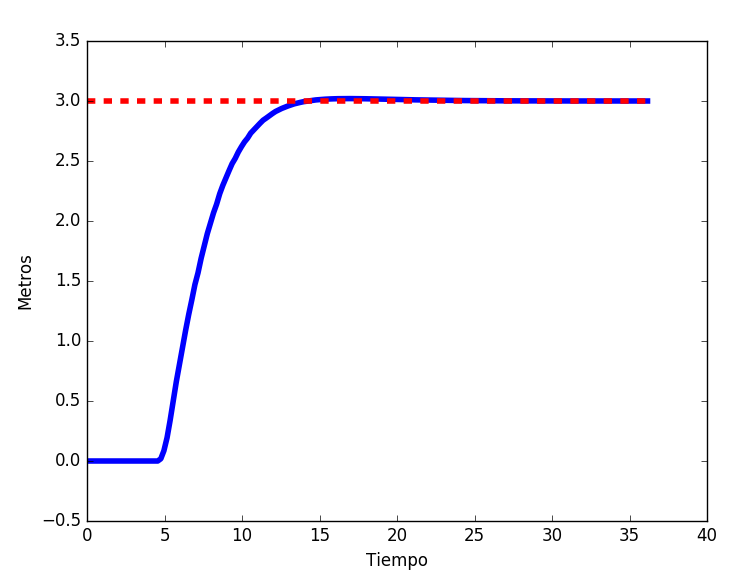
\includegraphics[width=.45\textwidth]{images/tvsxy_tesis.png}}
%        \subfigure[]{\label{fig:etiquetaB}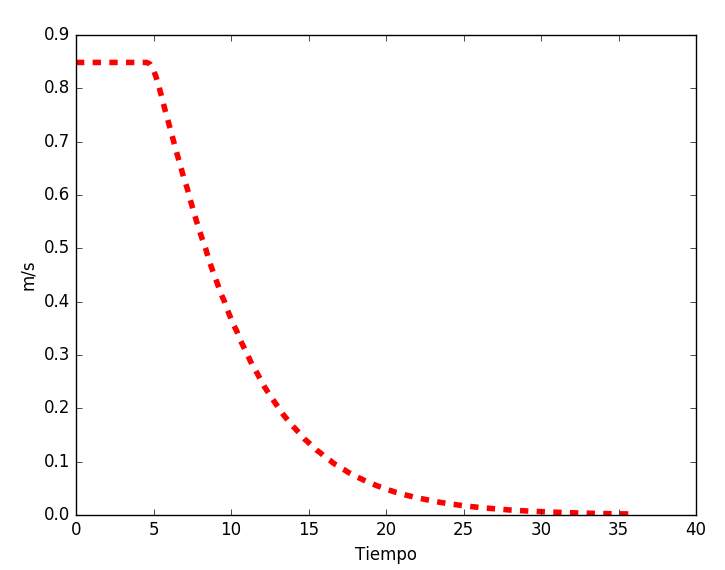
\includegraphics[width=.45\textwidth]{images/tvsv_tesis.png}}
%        \subfigure[]{\label{fig:etiquetaC}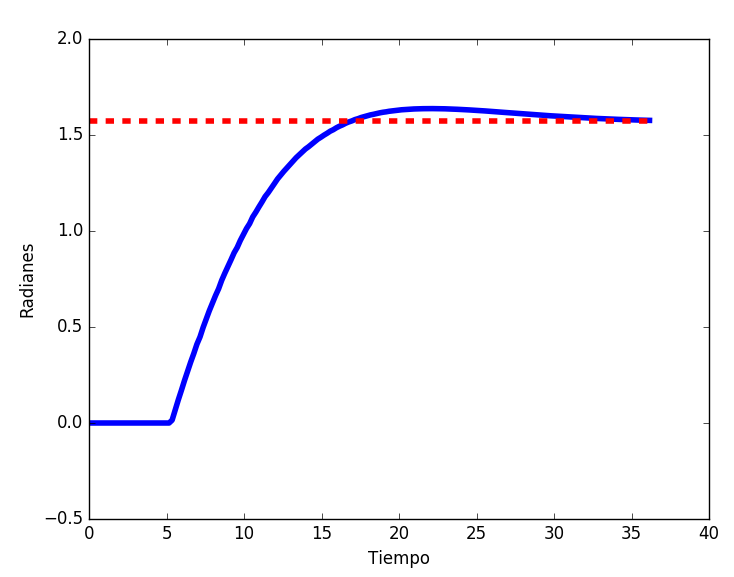
\includegraphics[width=.45\textwidth]{images/tvstheta_tesis.png}}
%        \subfigure[]{\label{fig:etiquetaD}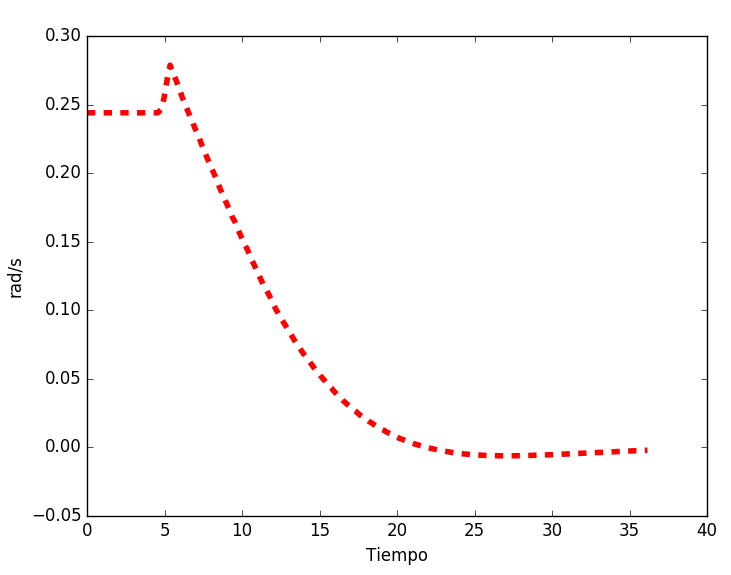
\includegraphics[width=.45\textwidth]{images/tvsomega_tesis.png}}
%    \end{center}
%  \captionsetup{font=footnotesize}
%    \caption{\label{f:PolarControl}Evolución temporal de las variables de estado usando el 
%    controlador polar para lograr una posición deseada dada por $x = 3, y = 3, 
%    \theta = 90$. En (a) se muestra la evolución temporal en la posición del eje x, en (b) 
%    se muestra la evolución de la velocidad lineal, en (c) se muestra la evolución de la
%    orientación y en (d) se muestra la evolución de la velocidad angular.}
%\end{figure}

\begin{figure}[ht!]
  \begin{tabular}{cc}
  %\centering
    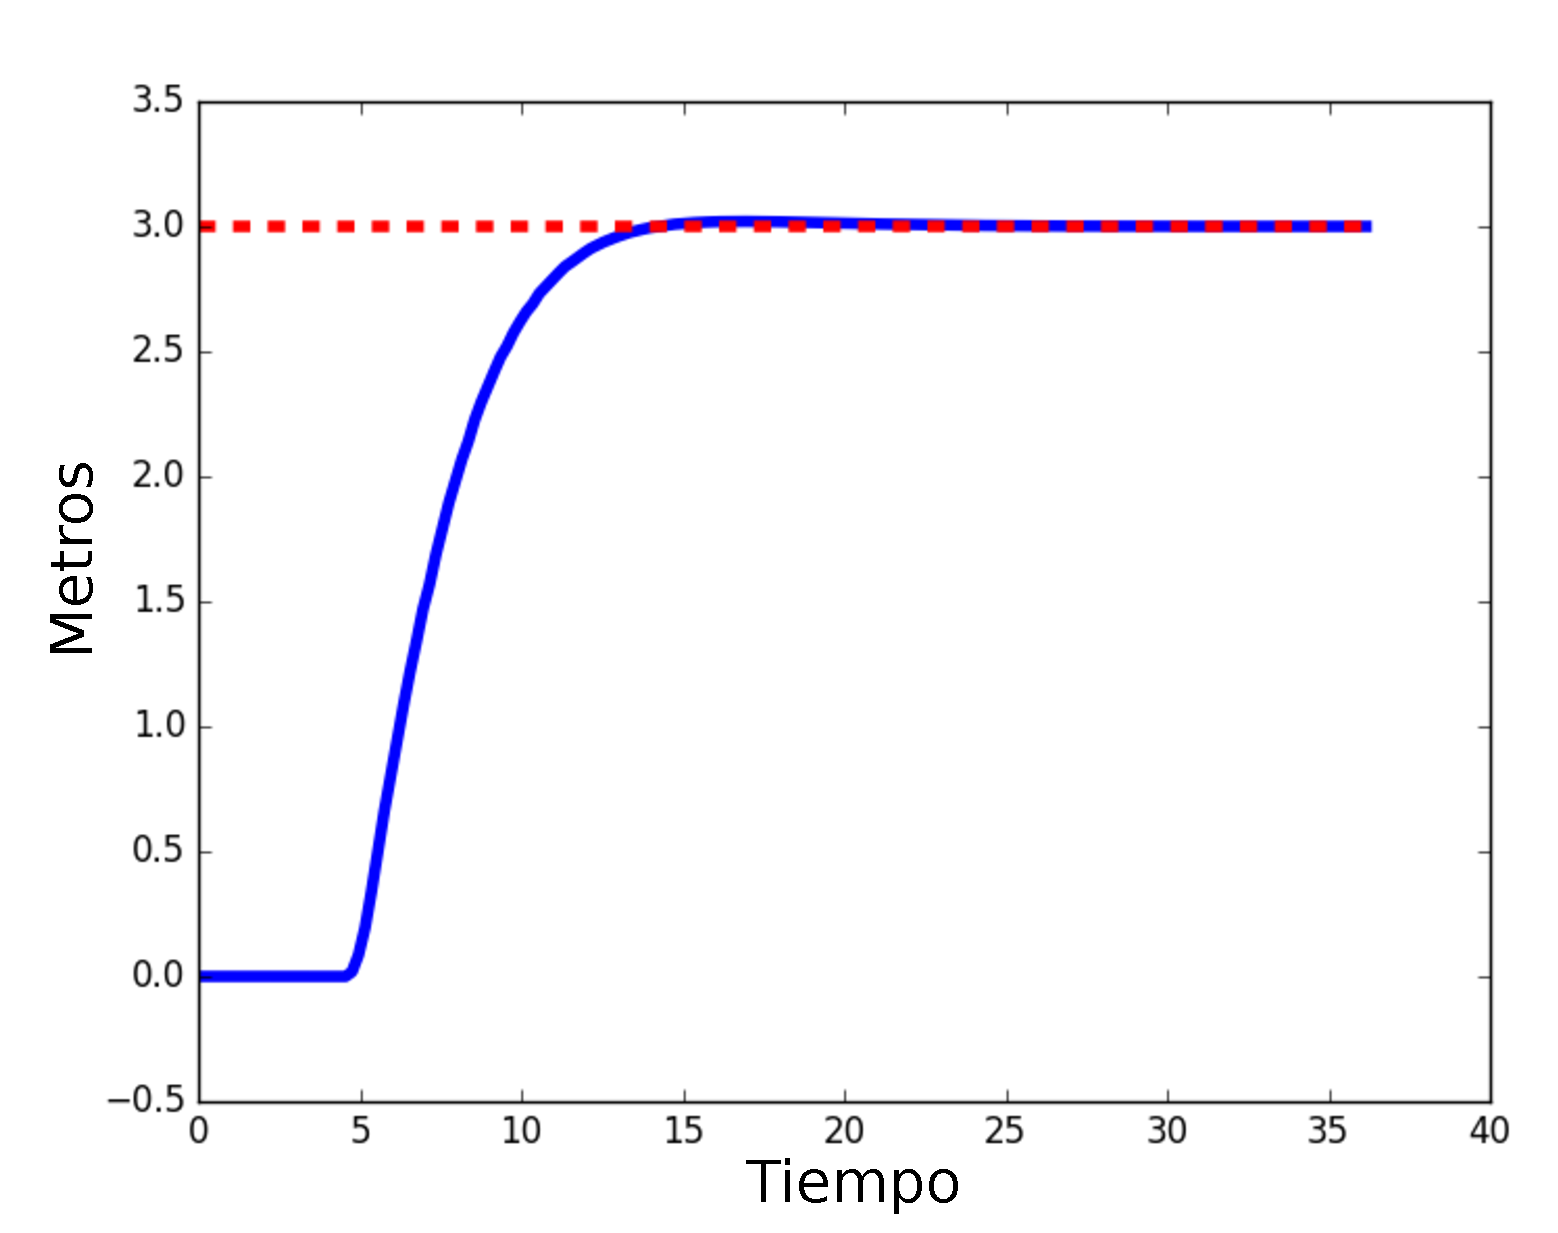
\includegraphics[width=.47\textwidth]{images/tvsxy_tesis.eps}&
    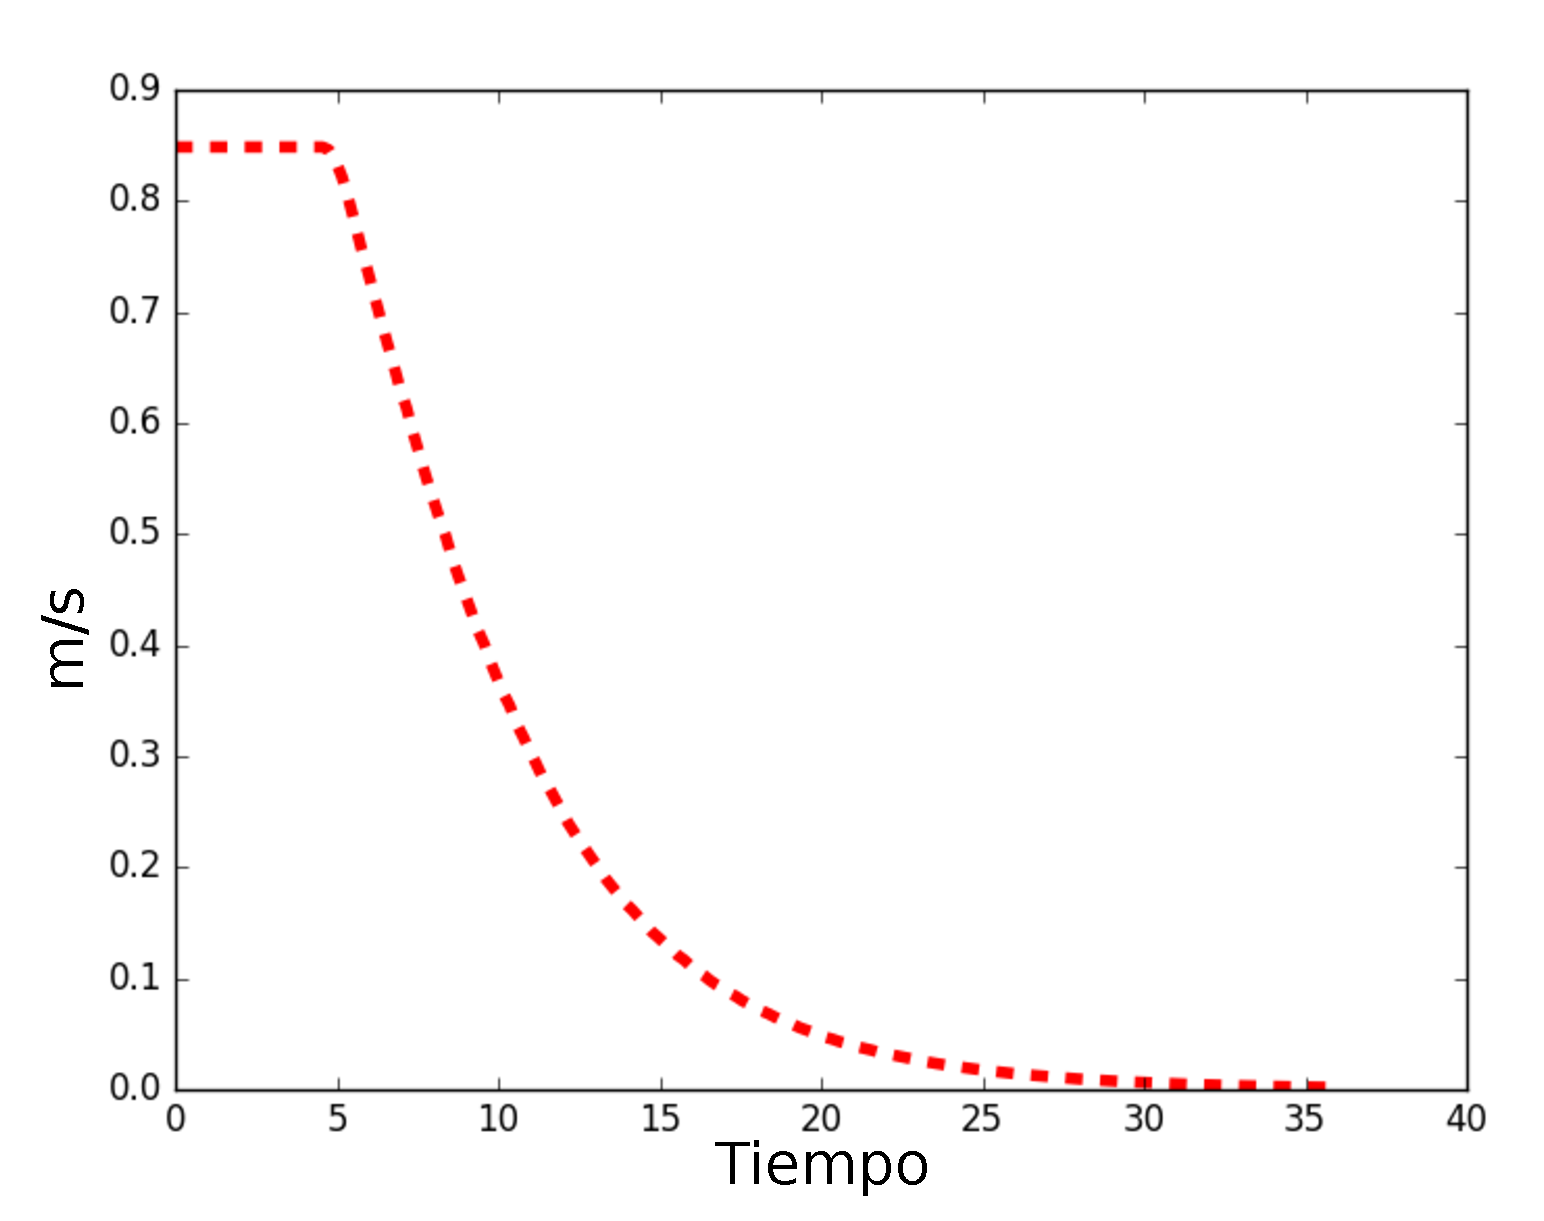
\includegraphics[width=.47\textwidth]{images/tvsv_tesis.eps}\\
    (a)&(b)\\
    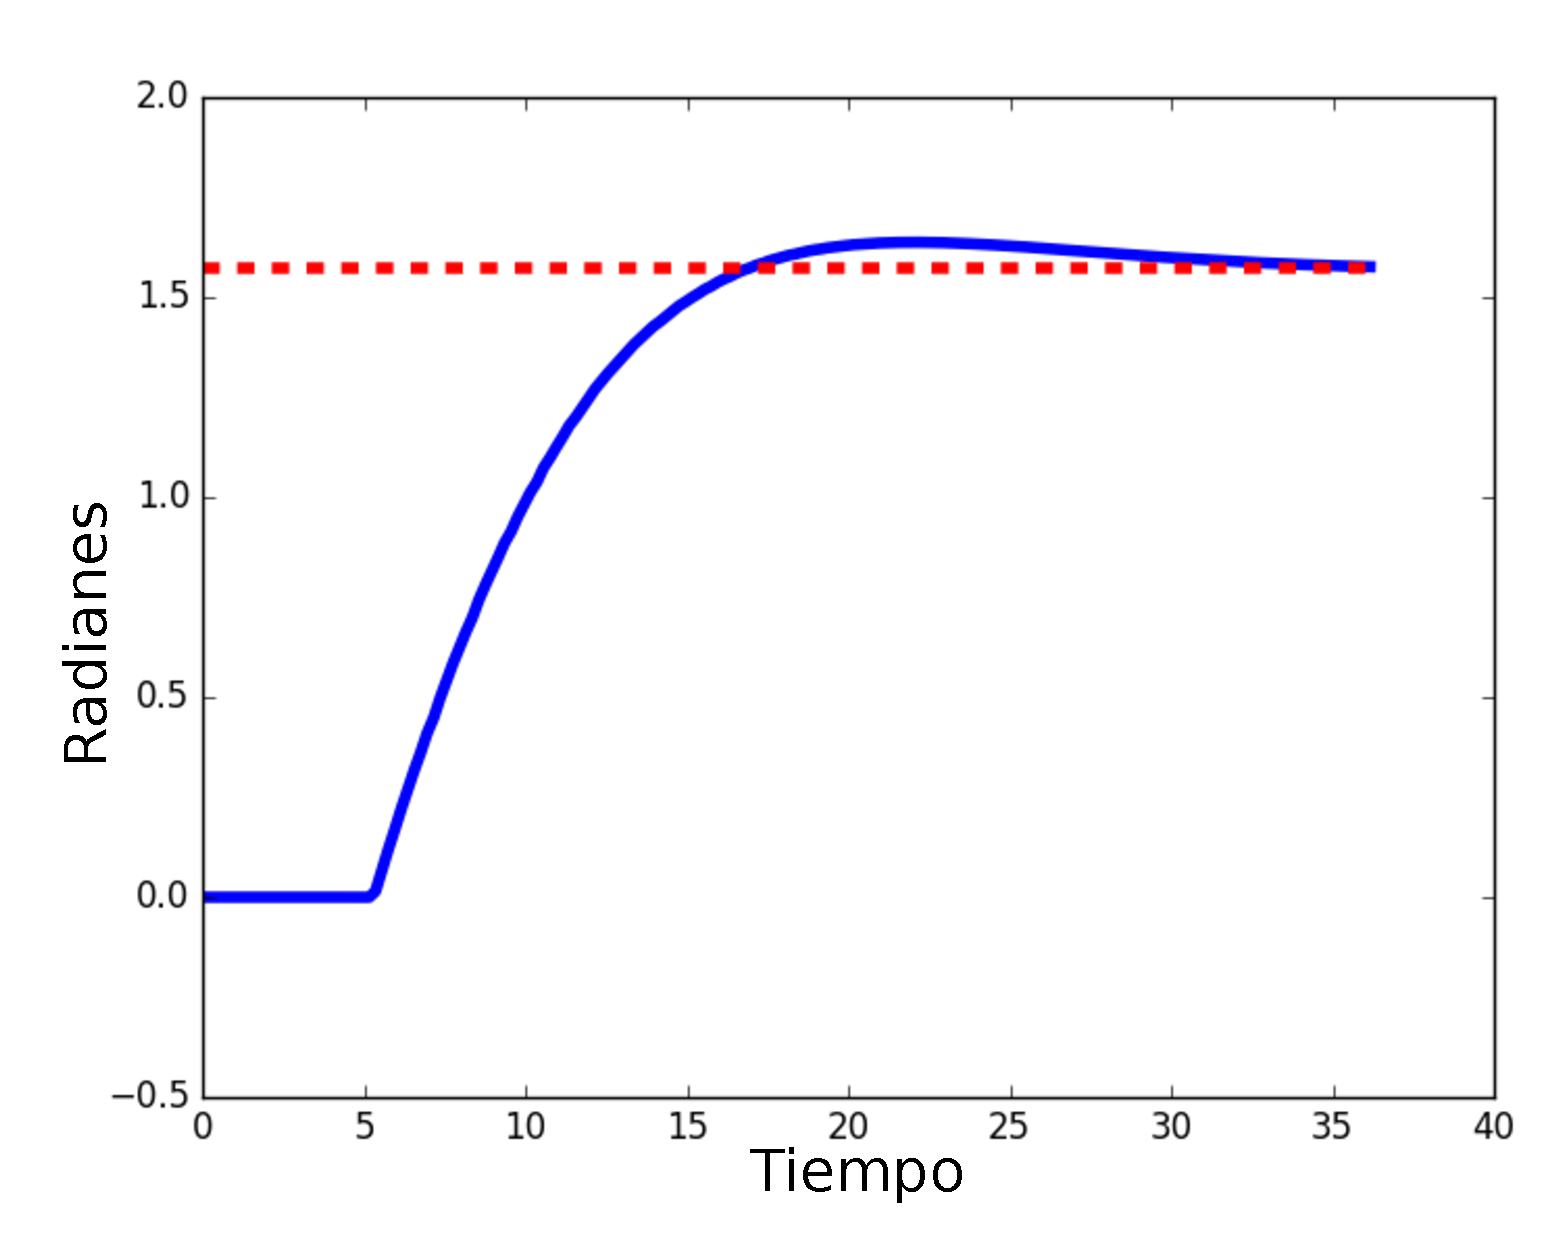
\includegraphics[width=.47\textwidth]{images/tvstheta_tesis.eps}&
    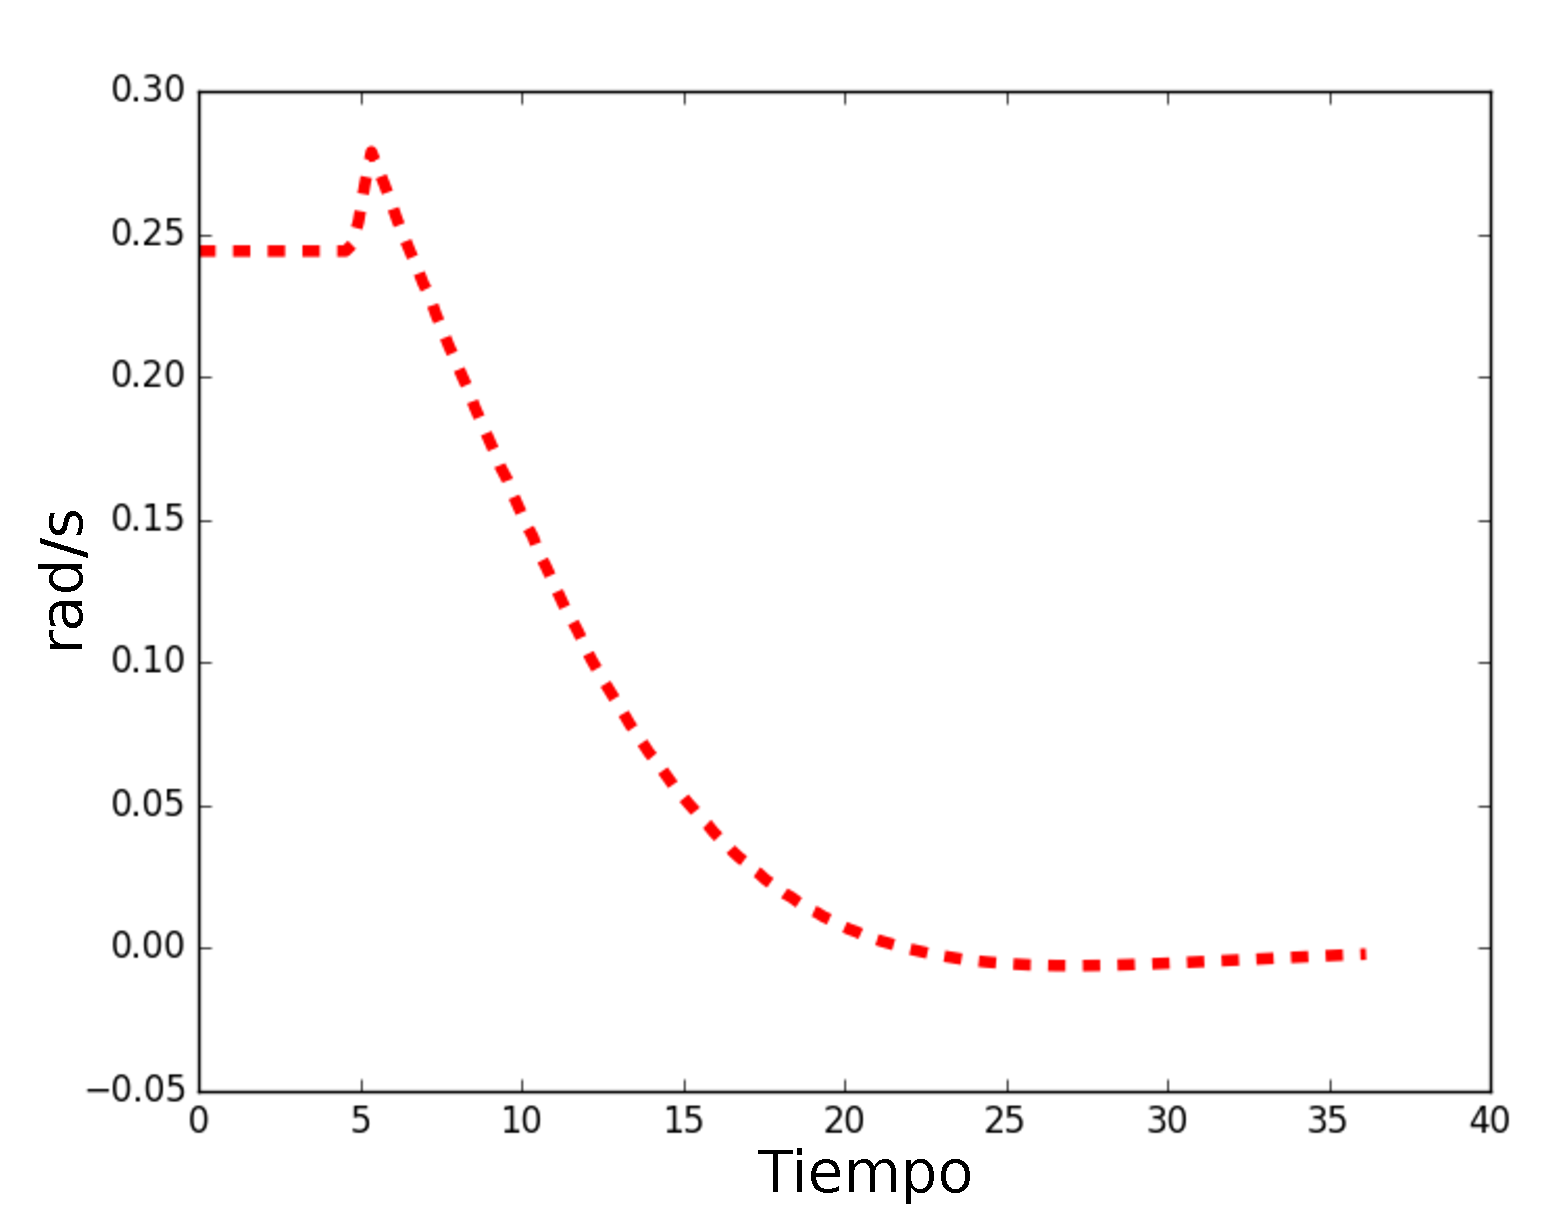
\includegraphics[width=.47\textwidth]{images/tvsomega_tesis.eps}\\
    (c)&(d)
  \end{tabular}
  \caption{Evolución temporal de las variables de estado usando el controlador polar para 
  lograr una posición deseada dada por $x = 3, y = 3, \theta = 90$. En (a) se muestra la 
  evolución temporal en la posición del eje x, en (b) se muestra la evolución de la 
  velocidad lineal, en (c) se muestra la evolución de la orientación y en (d) se muestra 
  la evolución de la velocidad angular.}
  \label{f:PolarControl}
\end{figure}


%\begin{figure}%[ht!]
%  \centering \footnotesize
%  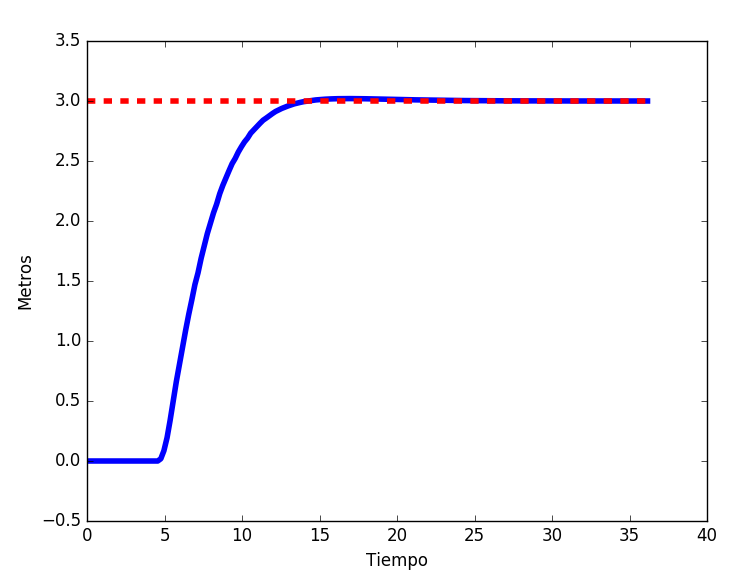
\includegraphics[width=0.49\textwidth]{images/tvsxy_tesis.png}
%  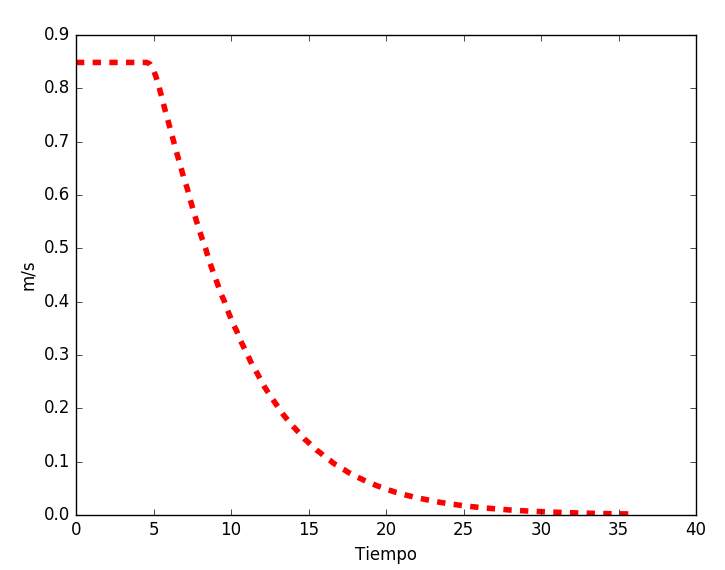
\includegraphics[width=0.49\textwidth]{images/tvsv_tesis.png}
%  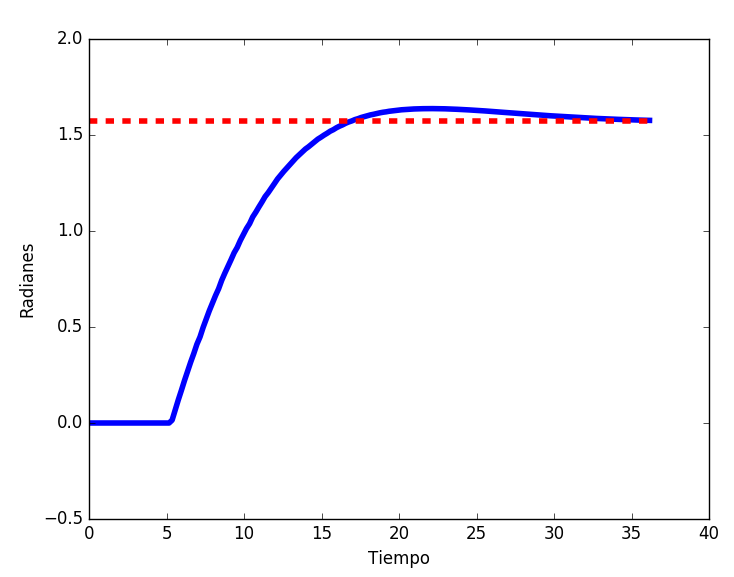
\includegraphics[width=0.49\textwidth]{images/tvstheta_tesis.png}
%  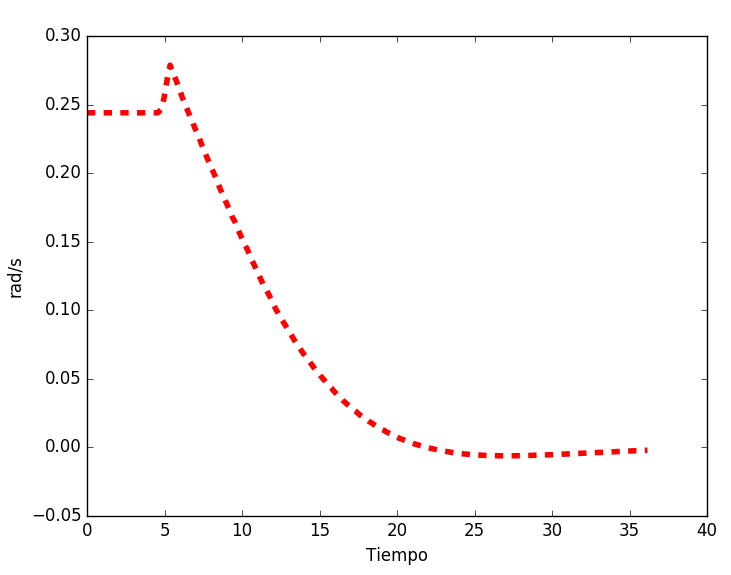
\includegraphics[width=0.49\textwidth]{images/tvsomega_tesis.png}
%  \captionsetup{font=footnotesize}
%  \caption{Evolución temporal de las variables de estado usando el controlador polar 
%  para lograr una posición deseada dada por $x = 3, y = 3, \theta = 90$}
%  \label{f:PolarControl}
%\end{figure}
Para probar el controlador polar, se usó una simulación dinámica en Gazebo con el robot 
Kobuki sin obstáculos, y las variables de estado que incluyen velocidad, posición y 
orientación se obtuvieron en línea a partir de la odometría simulada. Usando la información 
de esta odometría, el controlador se aplicó en línea. Para estas pruebas, la posición deseada
es $(x = 3, y = 3)$ y la orientación deseada $\theta = 90^{\circ}$. La Figura 
\ref{f:PolarControl}a muestra la evolución temporal de la posición ($x$) donde 
se logra una convergencia a la posición deseada en menos de 20 segundos. Esto se debe a 
la distancia hacia el obstáculo. Diferentes distancias conducen a diferentes tiempos de 
convergencia, y la tasa de convergencia también se puede modificar cambiando las 
ganancias en \ref{eqn:w} para la velocidad angular, y en \ref{eqn:v} para la velocidad 
lineal. Las otras subfiguras en la Figura \ref{f:PolarControl} muestran la evolución 
temporal de la velocidad lineal en $x$, la orientación y la velocidad angular. Para la 
orientación, hay un sobreimpulso que se debe a la excesiva dependencia del controlador 
en la posición en lugar de la orientación (ver Figura \ref{f:PolarControl}c).
%\section{An\'alisis del mapa obtenido}
%\section{Resultados en un ambiente real}
\section{Resultados del Sistema de Navegación}
\begin{figure}%[ht!]
  \centering
  \begin{tabular}{cc}
      %\subfigure[Fuerzas de atracción aplicado al robot móvil]{\label{fig:etiquetaA}\includegraphics
      %[width=.49\textwidth]{images/attr_kbki.eps}}
     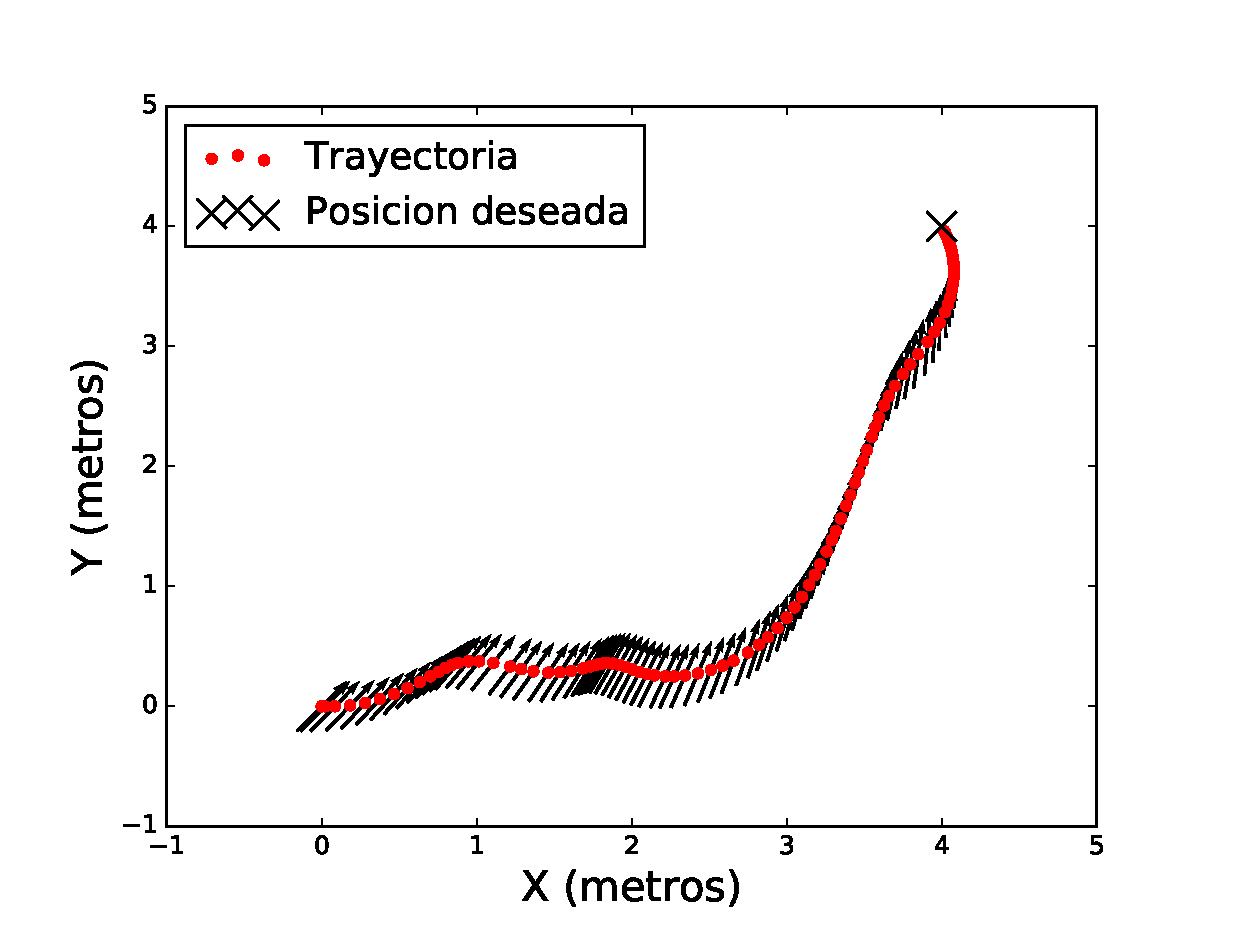
\includegraphics[width=0.51\linewidth]{images/attr_kbki.eps}&
      %\subfigure[Fuerzas de repulsión aplicado al robot móvil]{\label{fig:etiquetaB}\includegraphics
      %[width=.49\textwidth]{images/rep_kbki.eps}}
     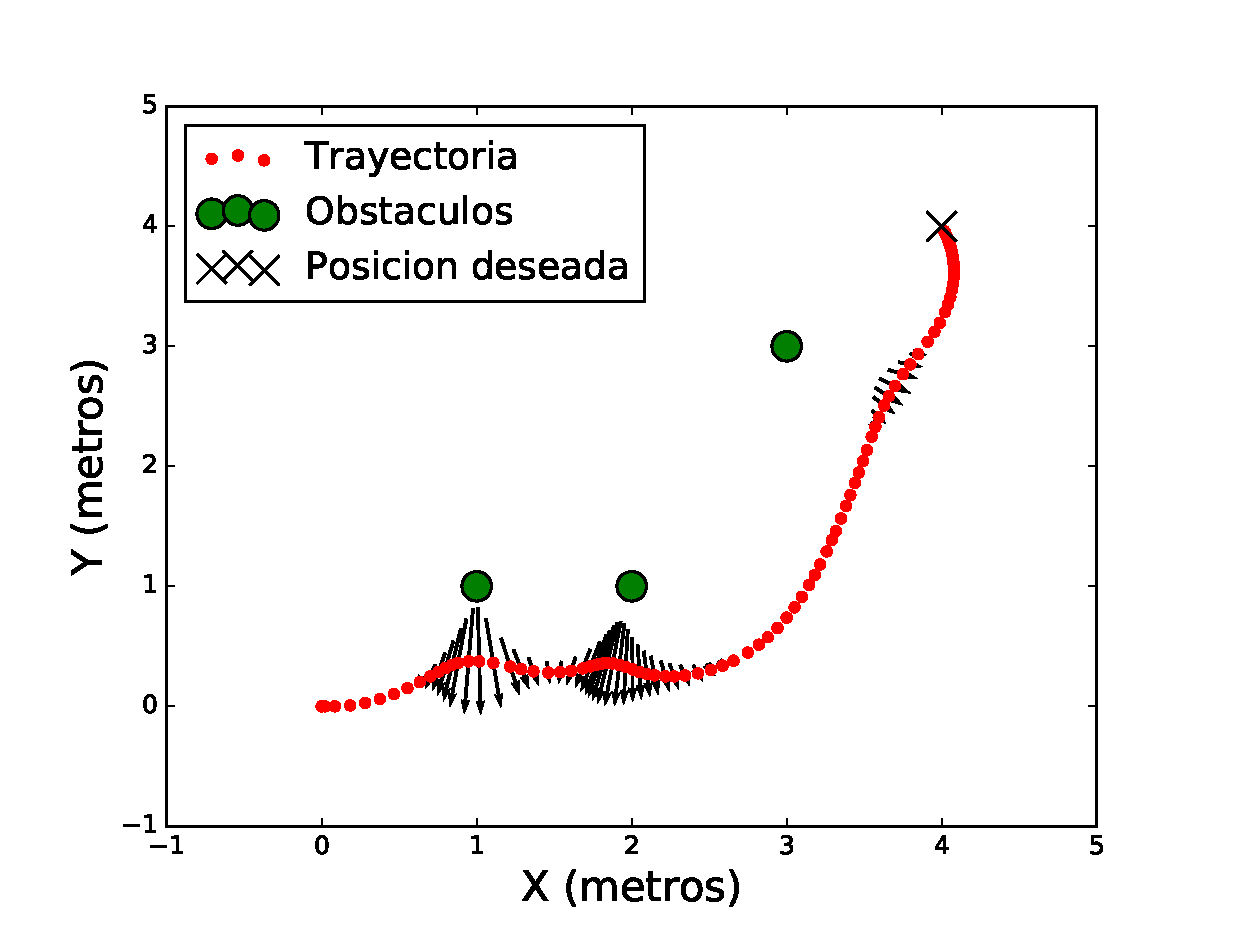
\includegraphics[width=0.51\linewidth]{images/rep_kbki.eps}\\
    (a) & (b)\\
    \multicolumn{2}{c}{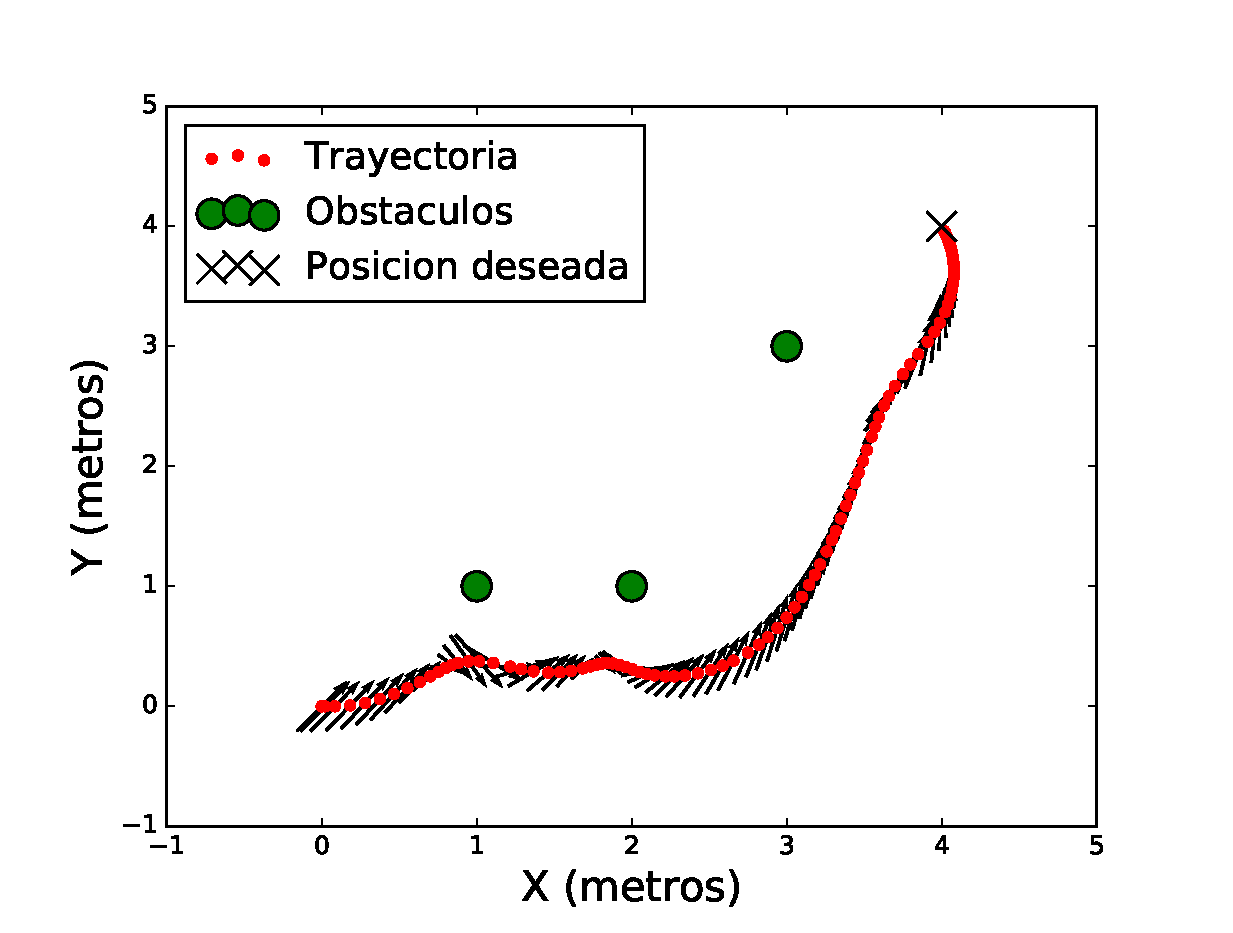
\includegraphics[width=0.52\linewidth]{images/nav_kbki.eps}}\\
      %\subfigure[Fuerzas de navegación aplicado al robot móvil]{\label{fig:etiquetaC}\includegraphics
      %[width=.49\textwidth]{images/nav_kbki.eps}}
    \multicolumn{2}{c}{(c)}
  \end{tabular}
 
  \caption{Navegación autónoma implementada en el robot diferencial Kobuki. En (a) se muestra
  las fuerzas de atracción que llevan al Kobuki a la posición deseada, en (b) se muestra las 
  fuerzas de repulsión que evitan que el robot diferencial se choque con los obstáculos y en 
  (c) se muestra las fuerzas de navegación que genera la trayectoria del robot.}
  \label{f:kbki_APF}
 \end{figure}
%\begin{figure}%[ht!]
%  \centering \footnotesize
%  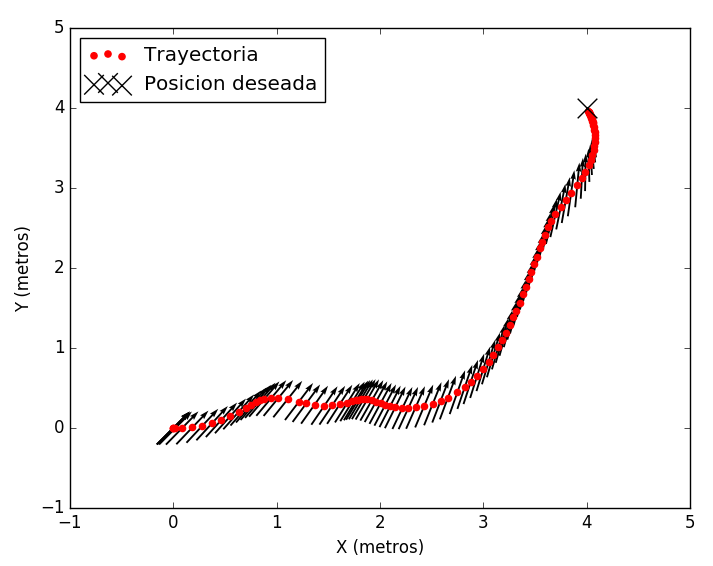
\includegraphics[width=0.61\textwidth]{images/attr_kbki.png}
%  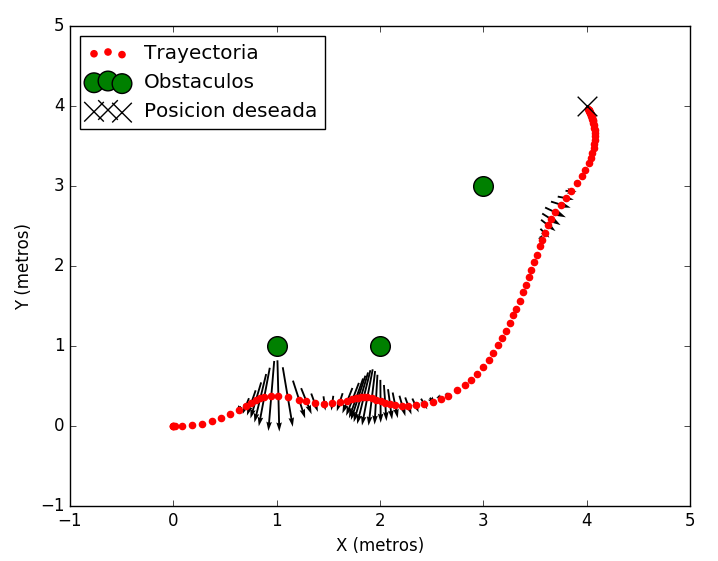
\includegraphics[width=0.60\textwidth]{images/rep_kbki.png}
%  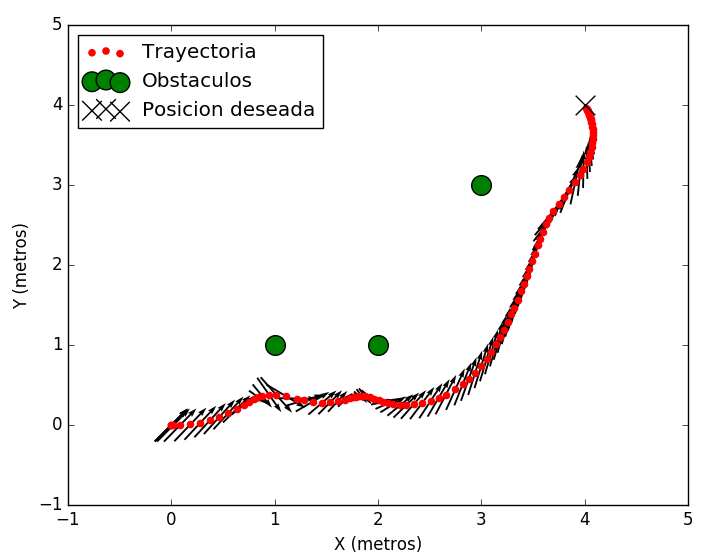
\includegraphics[width=0.60\textwidth]{images/nav_kbki.png}
%  \captionsetup{font=footnotesize}
%  \caption{Navegación autónoma implementada en el robot diferencial Kobuki.}
%  \label{f:kbki_APF}
%\end{figure}
La metodología propuesta se implementó como un algoritmo iterativo en el robot Kobuki. 
Como se se describe en la sección \ref{sec:autonomia}, el algoritmo toma iterativamente 
posiciones deseadas  donde a través del campo potencial artificial y el controlador 
polar impulsan al robot a través de las posiciones requeridas. Se expuso al robot 
a diferentes obstáculos cuyas posiciones fueron conocidas a priori. La Figura 
\ref{f:kbki_APF}a muestra las fuerzas de atracción para cada posición (puntos rojos) en 
las que el algoritmo se itera en el entorno de dos dimensiones dentro del movimiento del 
robot. Para cada posición, el campo de potencial atractivo se puede ver con la dirección 
de las flechas. La Figura \ref{f:kbki_APF}b se compone de las fuerzas de repulsión basadas en 
los obstáculos que se muestran como marcadores verdes. Para cada obstáculo, la magnitud de 
las fuerzas aumenta cuando el robot está más cerca y su dirección señala los obstáculos, permitiendo 
que el robot los evite. La Figura \ref{f:kbki_APF}c muestra la superposición de ambas fuerzas 
con los obstáculos reales. Cada fuerza proporciona una posición deseada intermedia para el 
robot, que constituye la posición deseada continuamente actualizada para el controlador 
polar. Aunque las fuerzas cercanas a los obstáculos tienen un alto índice de cambio, la 
trayectoria es suave. Esto demuestra la efectividad del controlador polar a pesar de las 
características no holonómicas del robot.

\section{Resultados de la Navegación Autónoma con el Lídar en dos dimensiones}
\begin{figure}%[ht!]
  \centering \footnotesize
  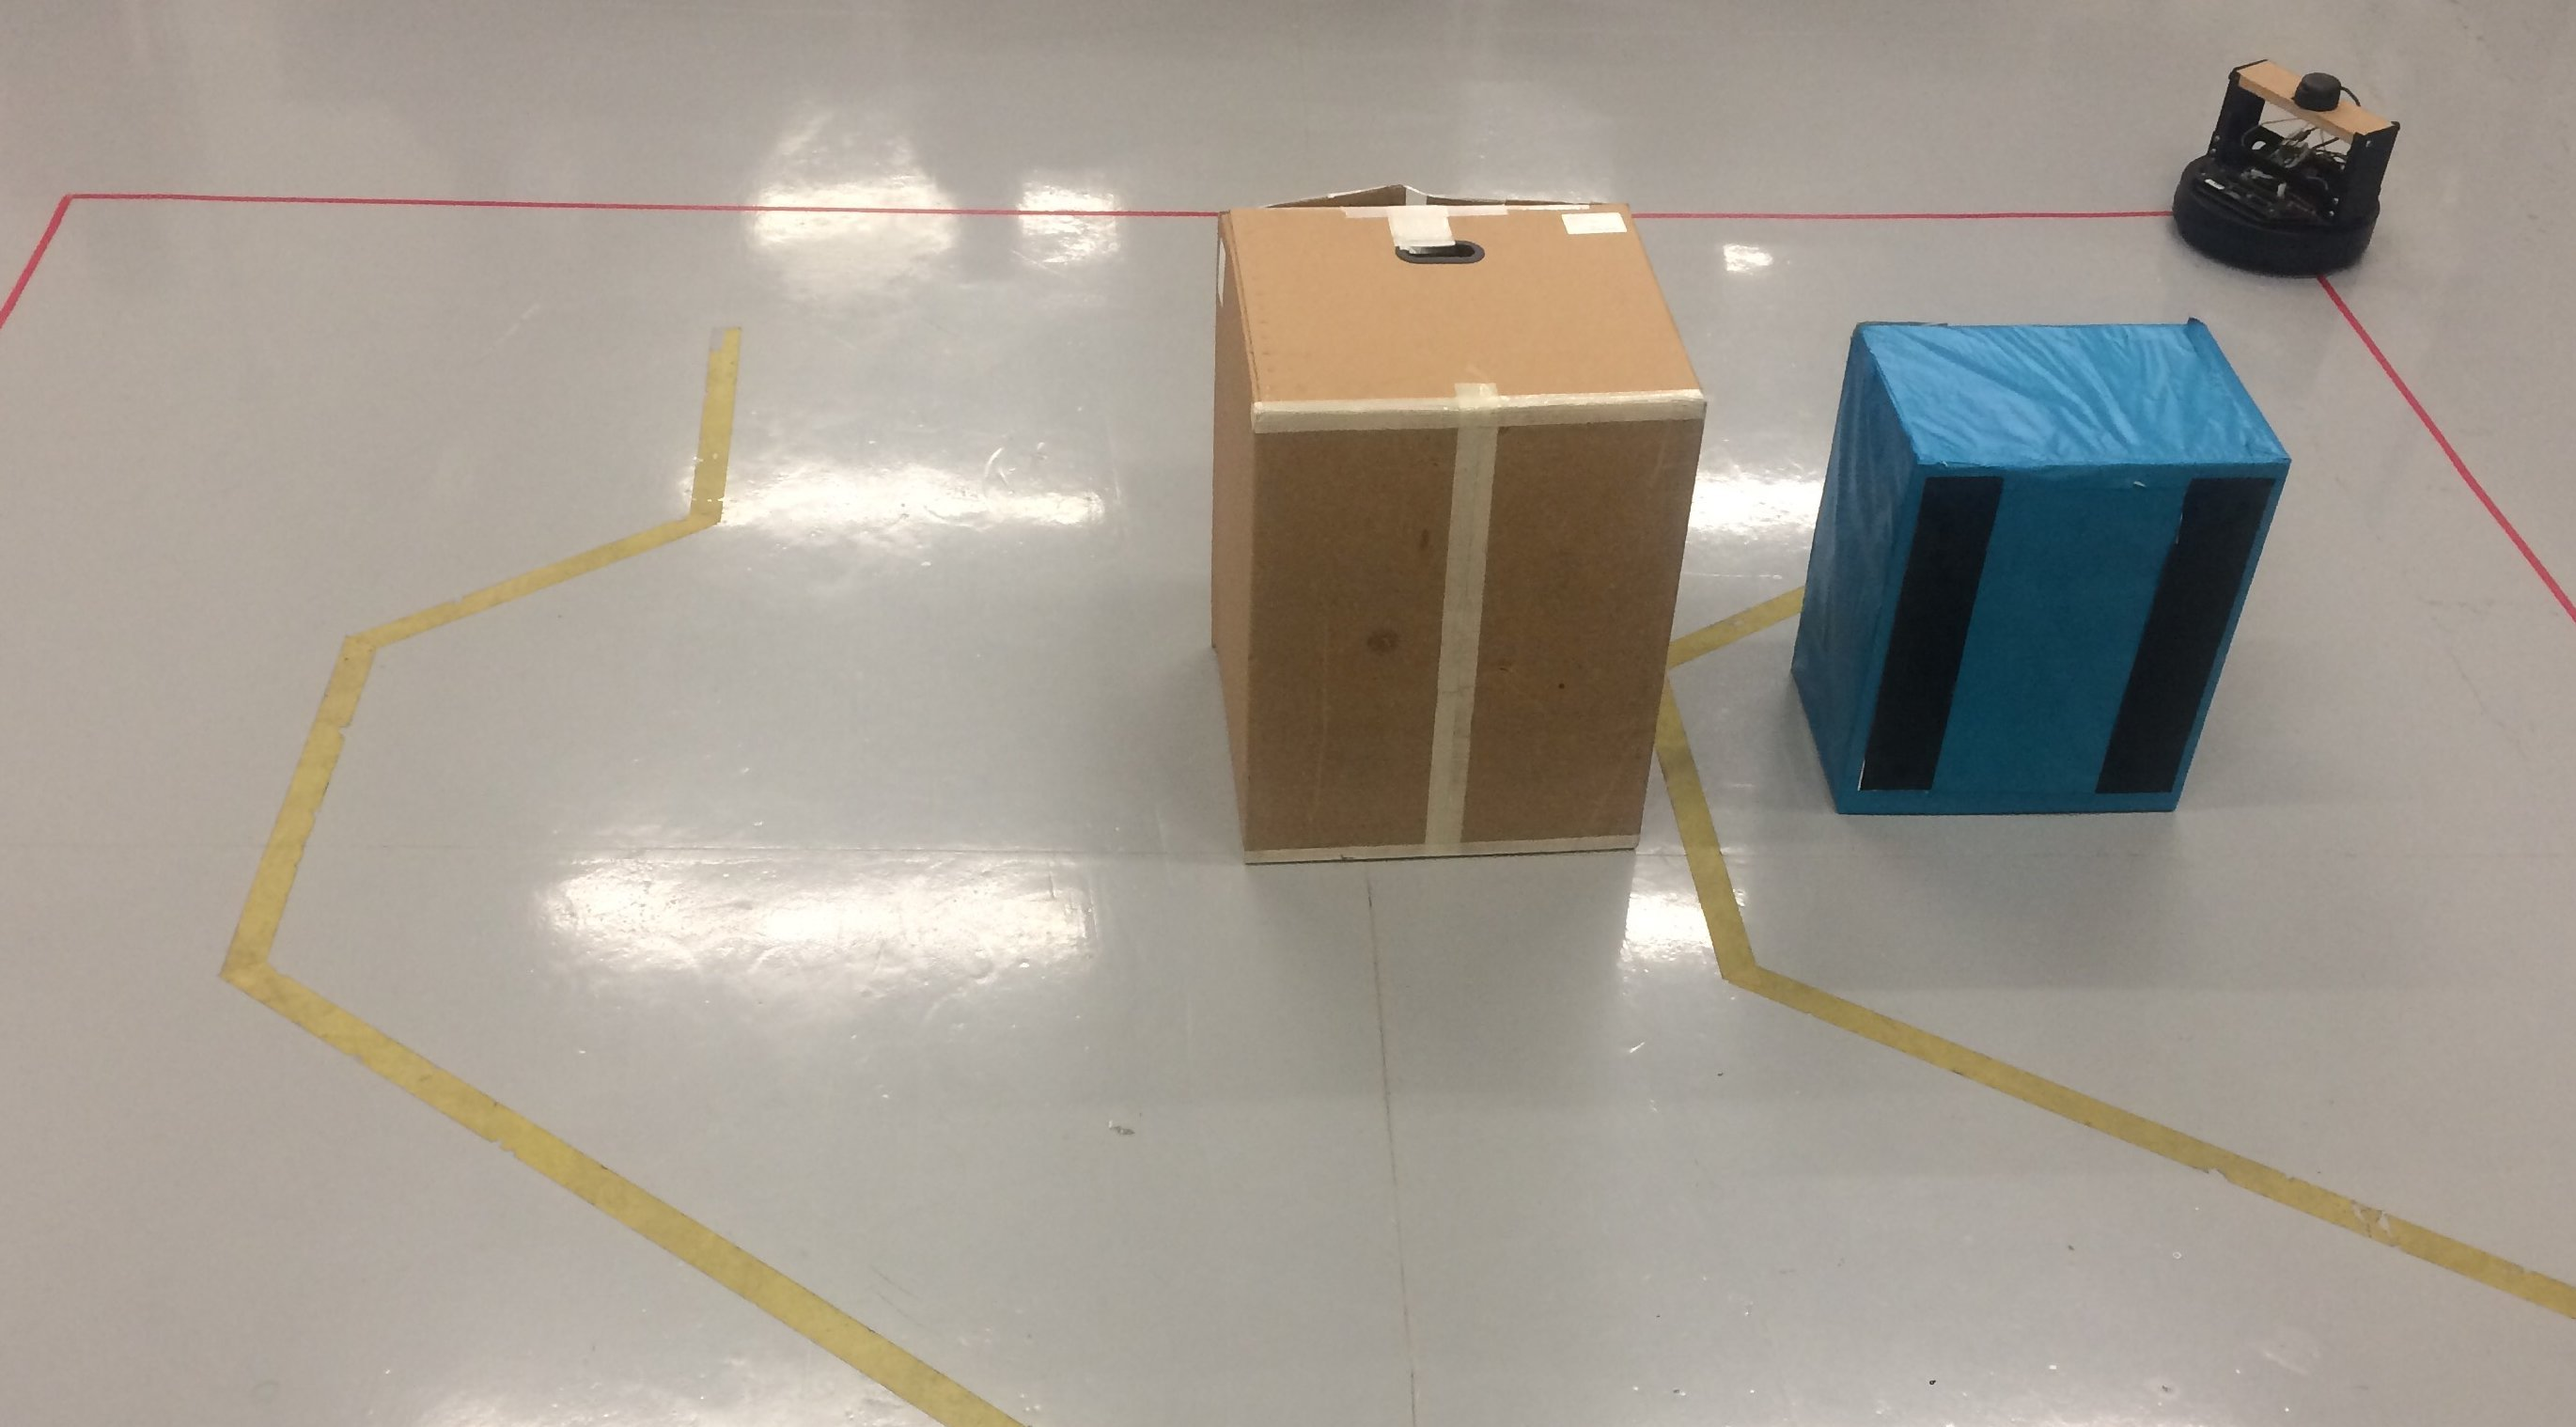
\includegraphics[width=0.80\textwidth]{images/kobuki_201.jpg}
  \captionsetup{font=footnotesize}
  \caption{Navegación autónoma del robot diferencial Kobuki, montado con un sensor lídar y dos cajas
  como obstáculos.}
  \label{fig:Kobuki201}
\end{figure}

%\begin{figure}[ht!]
%     \begin{center}
%        \subfigure[Fuerzas de atracción aplicado al robot móvil]{\label{fig:etiquetaA}\includegraphics
%        [width=.69\textwidth]{images/fattr_lidar_s.eps}}
%        \subfigure[Fuerzas de repulsión aplicado al robot móvil]{\label{fig:etiquetaB}\includegraphics
%        [width=.69\textwidth]{images/frep_lidar_s.png}}
%        \subfigure[Fuerzas de navegación aplicado al robot móvil]{\label{fig:etiquetaC}\includegraphics
%        [width=.69\textwidth]{images/fnav_lidar_s.png}}
%    \end{center}
\begin{figure}
  \centering
    \begin{tabular}{c}
      \multicolumn{1}{c}{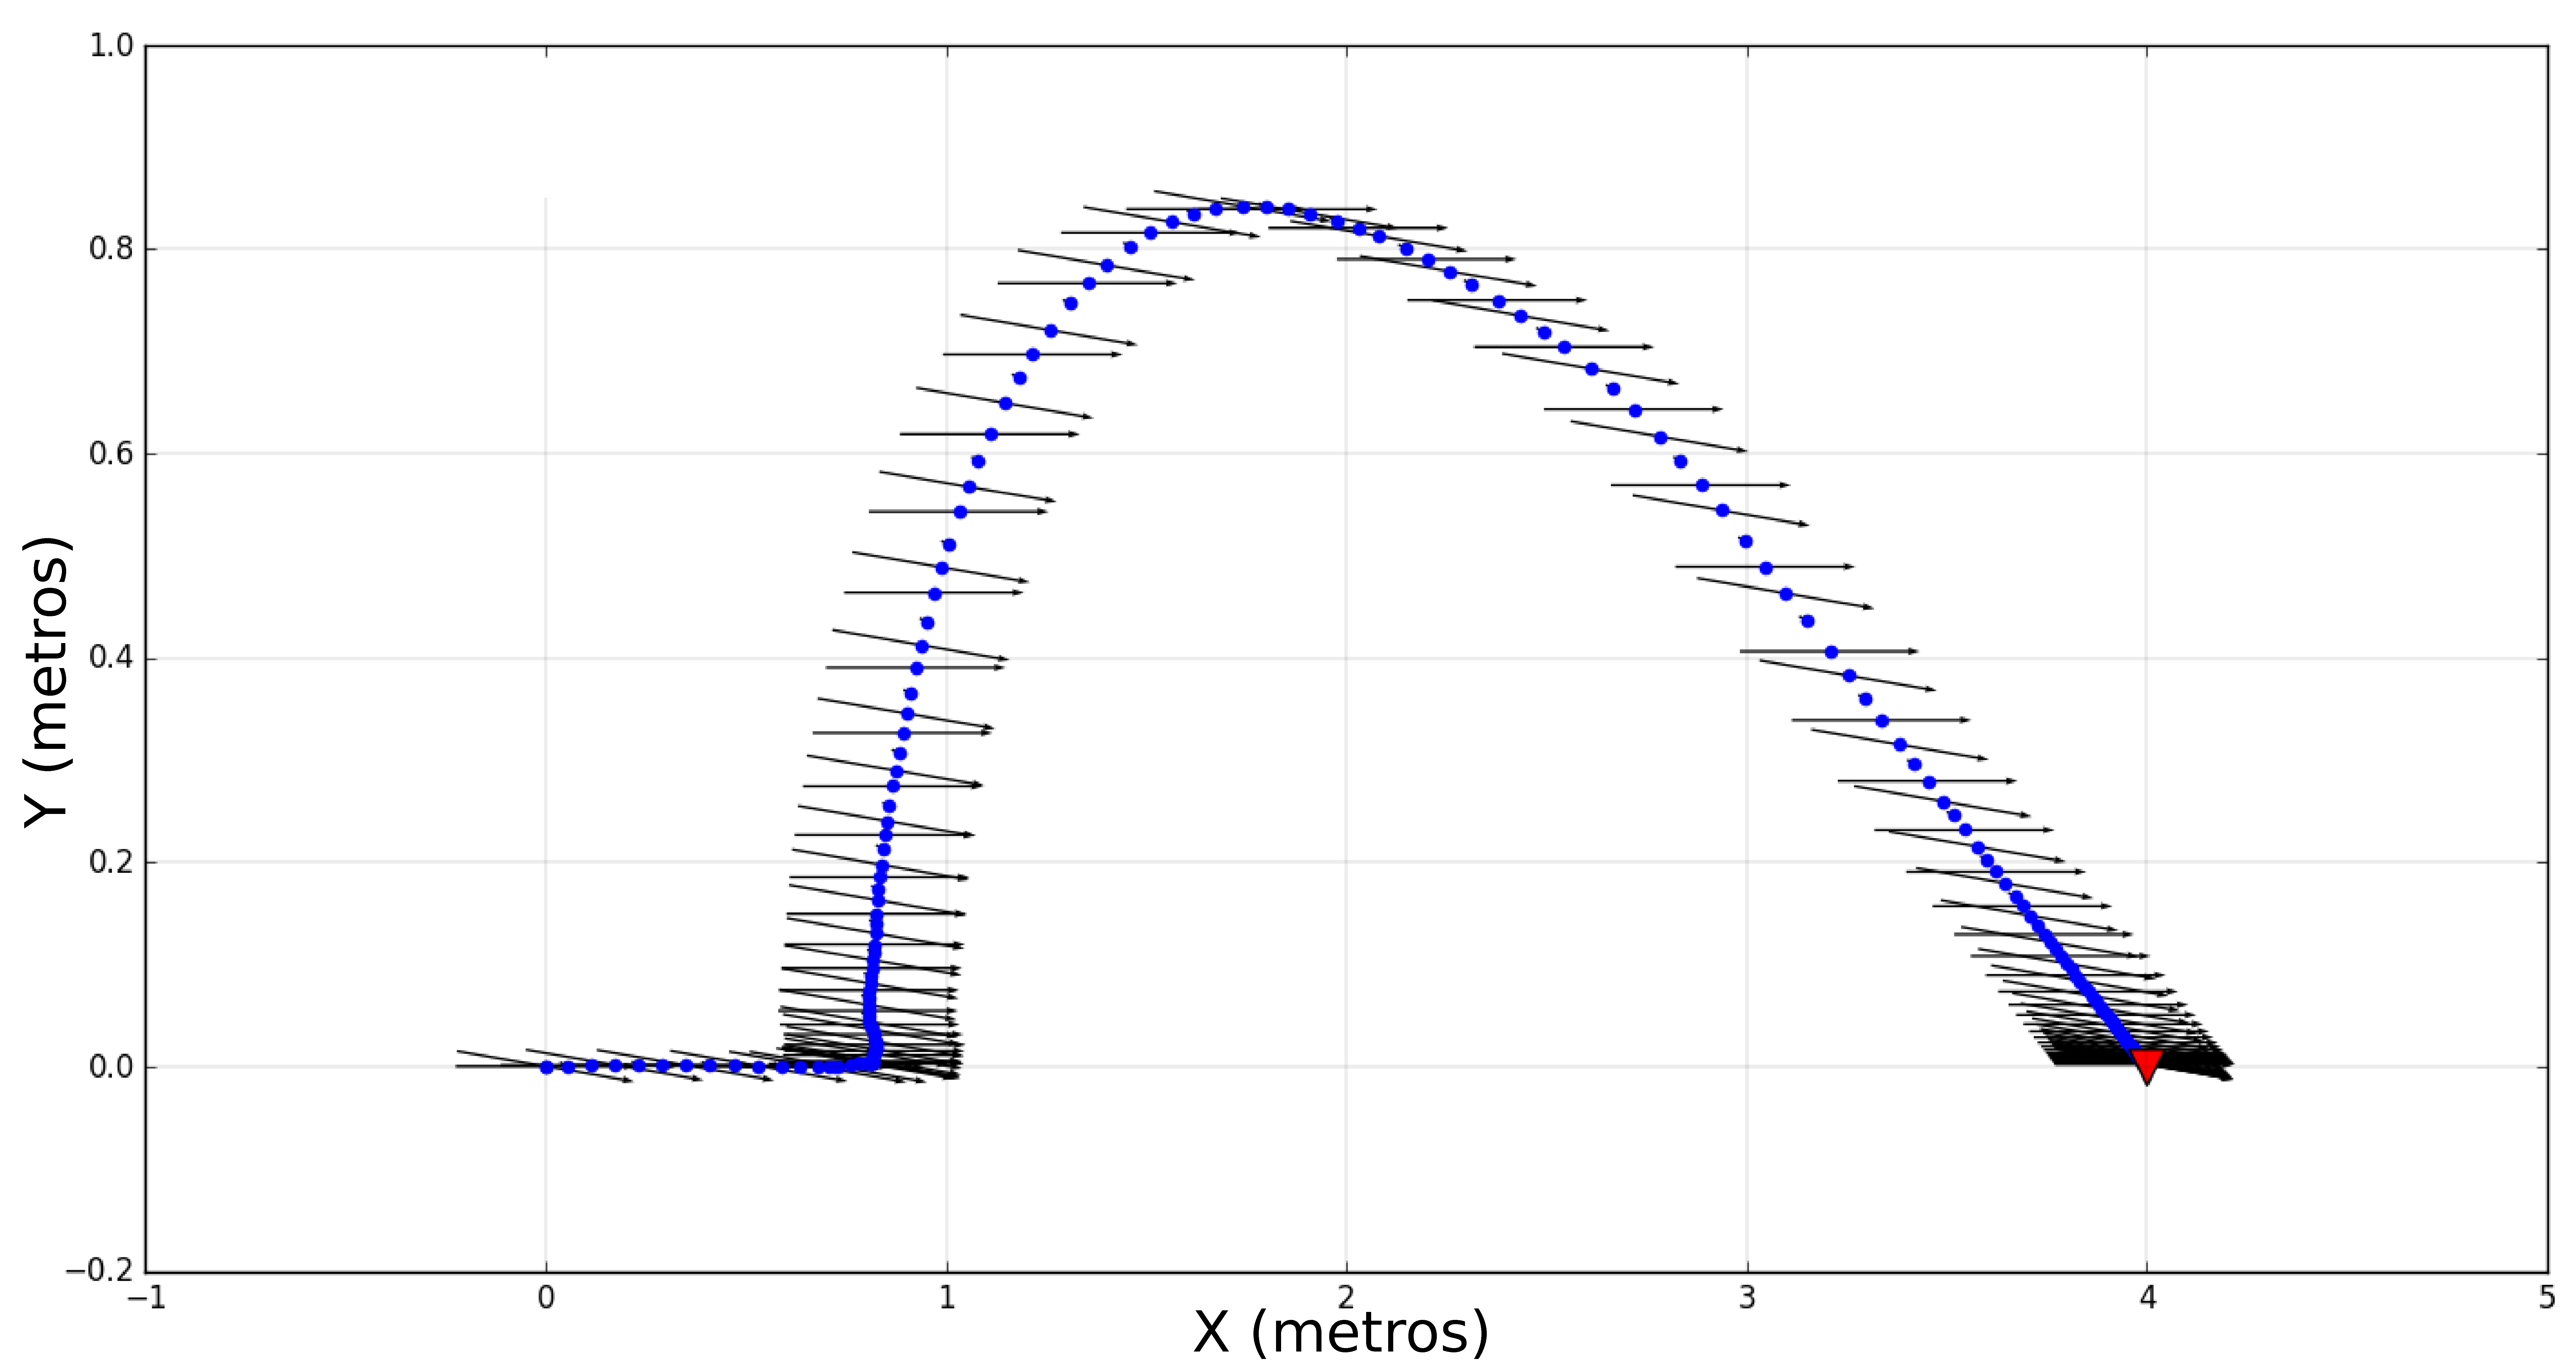
\includegraphics[width=.75\textwidth]{images/fattr_lidar_s.eps}}\\
      \multicolumn{1}{c}{(a)}\\
      \multicolumn{1}{c}{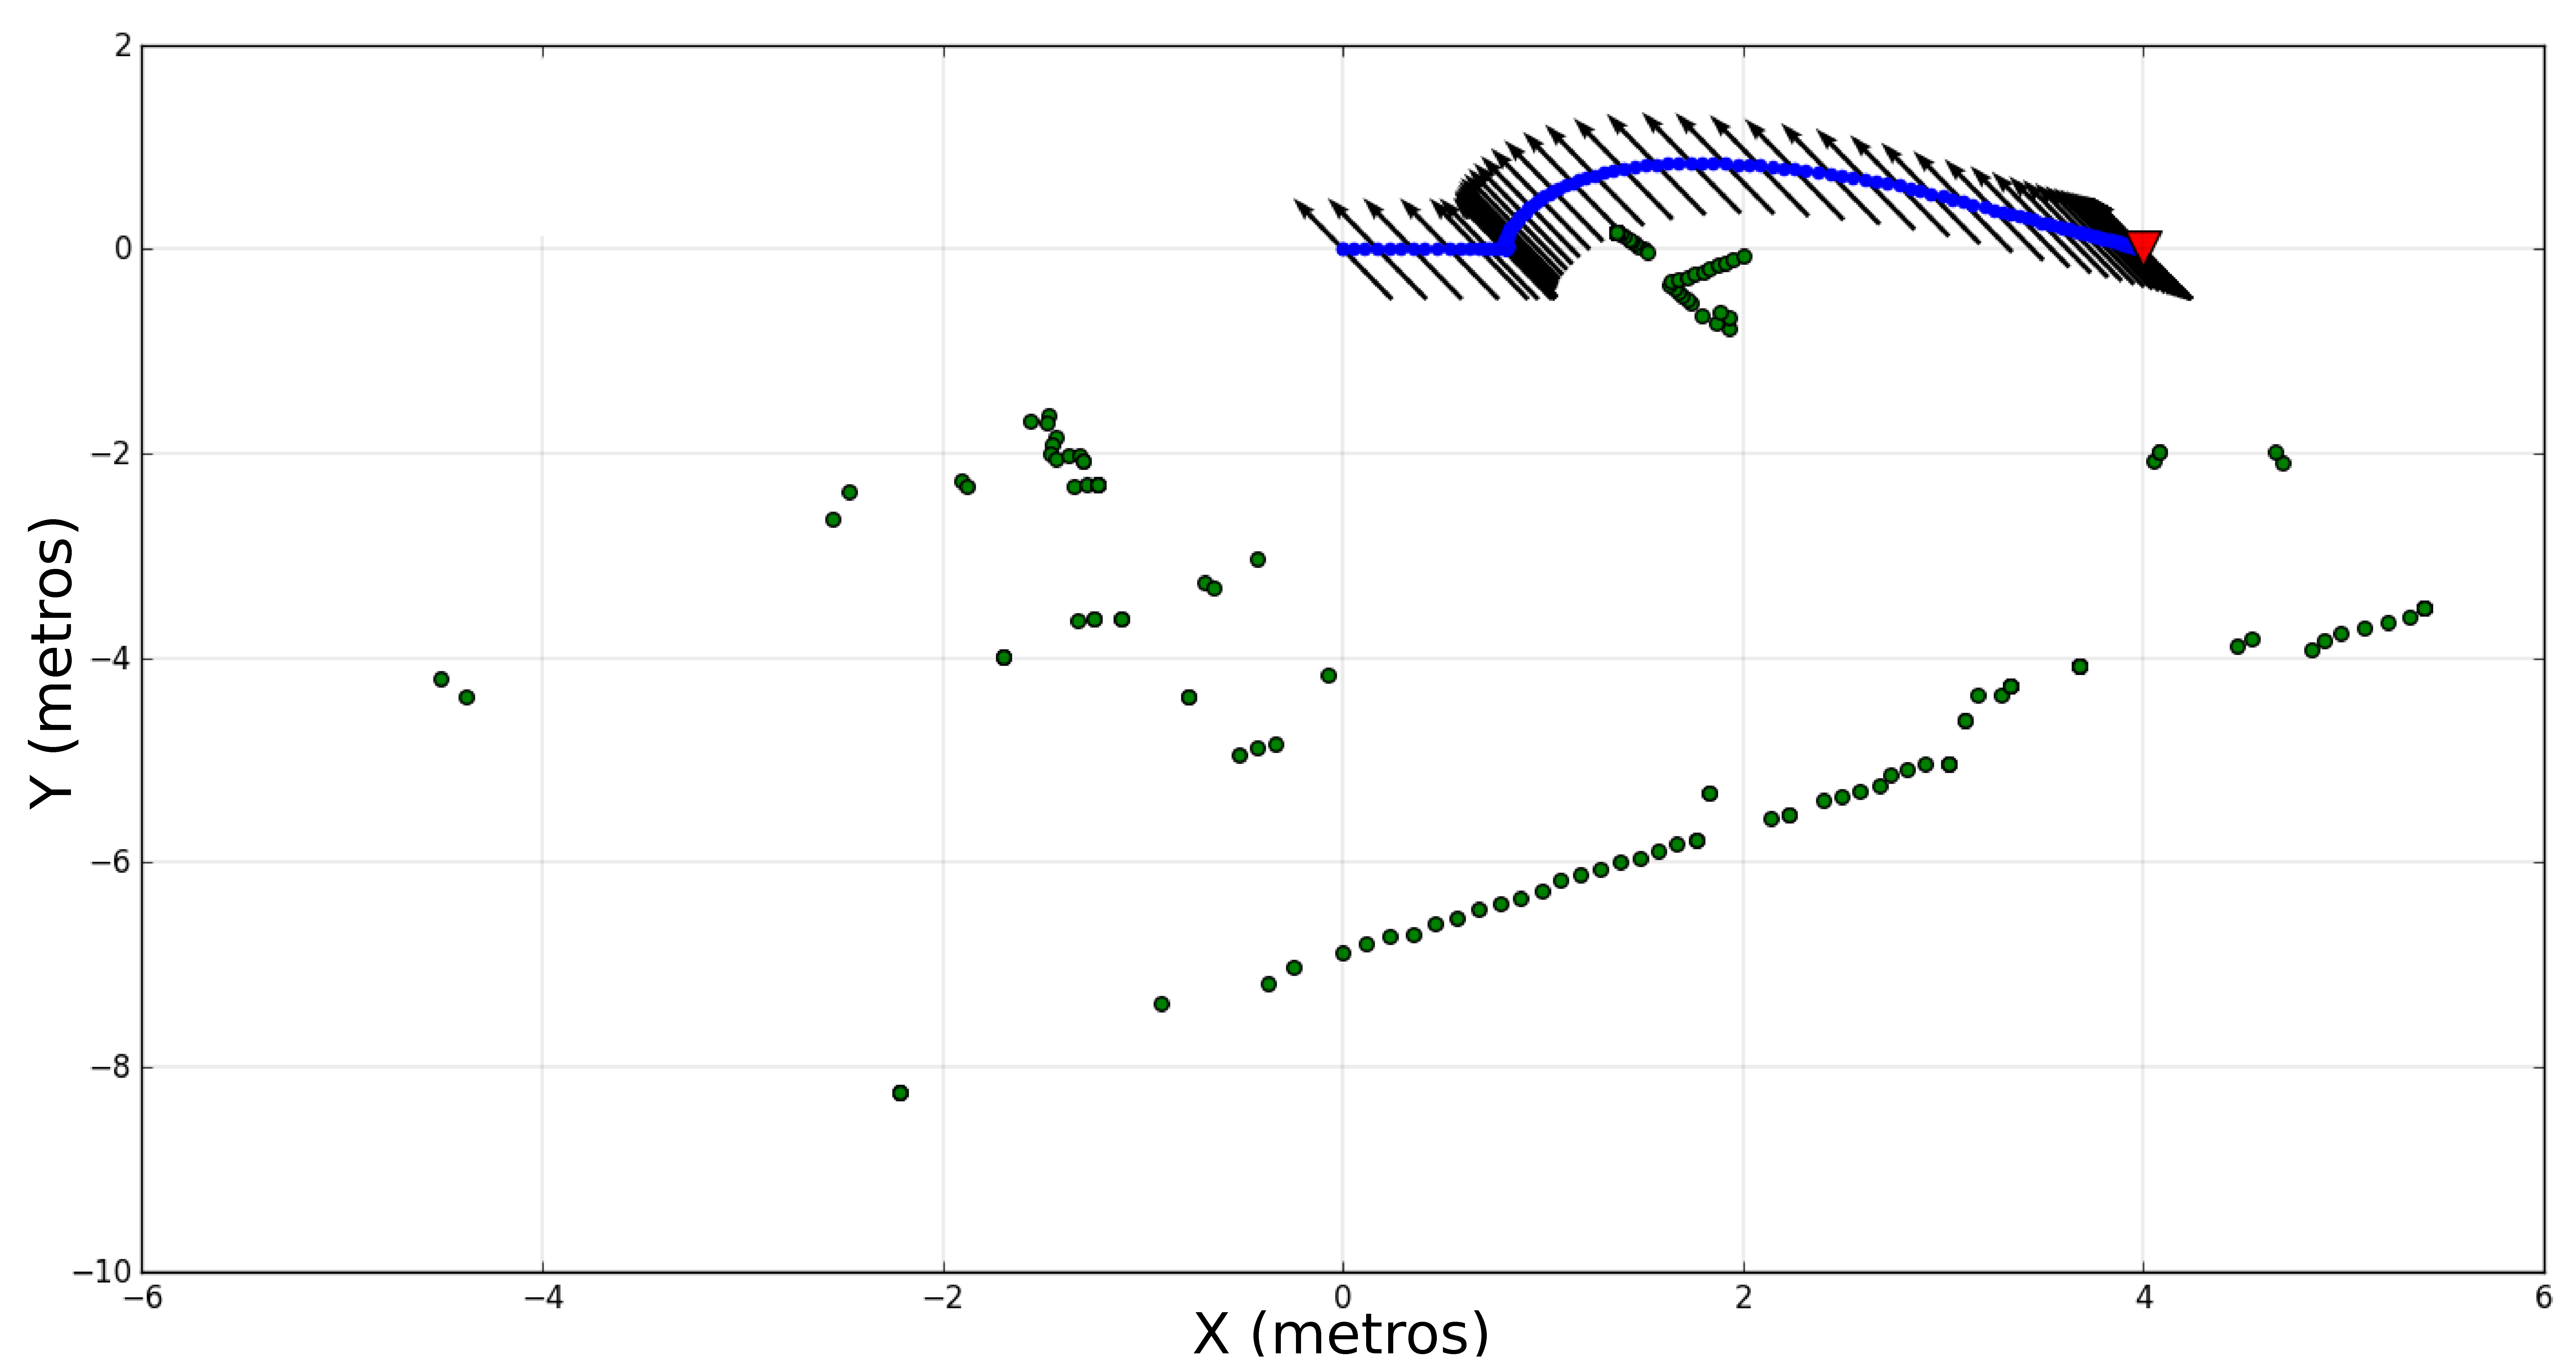
\includegraphics[width=.75\textwidth]{images/frep_lidar_s.eps}}\\
      \multicolumn{1}{c}{(b)}\\
      \multicolumn{1}{c}{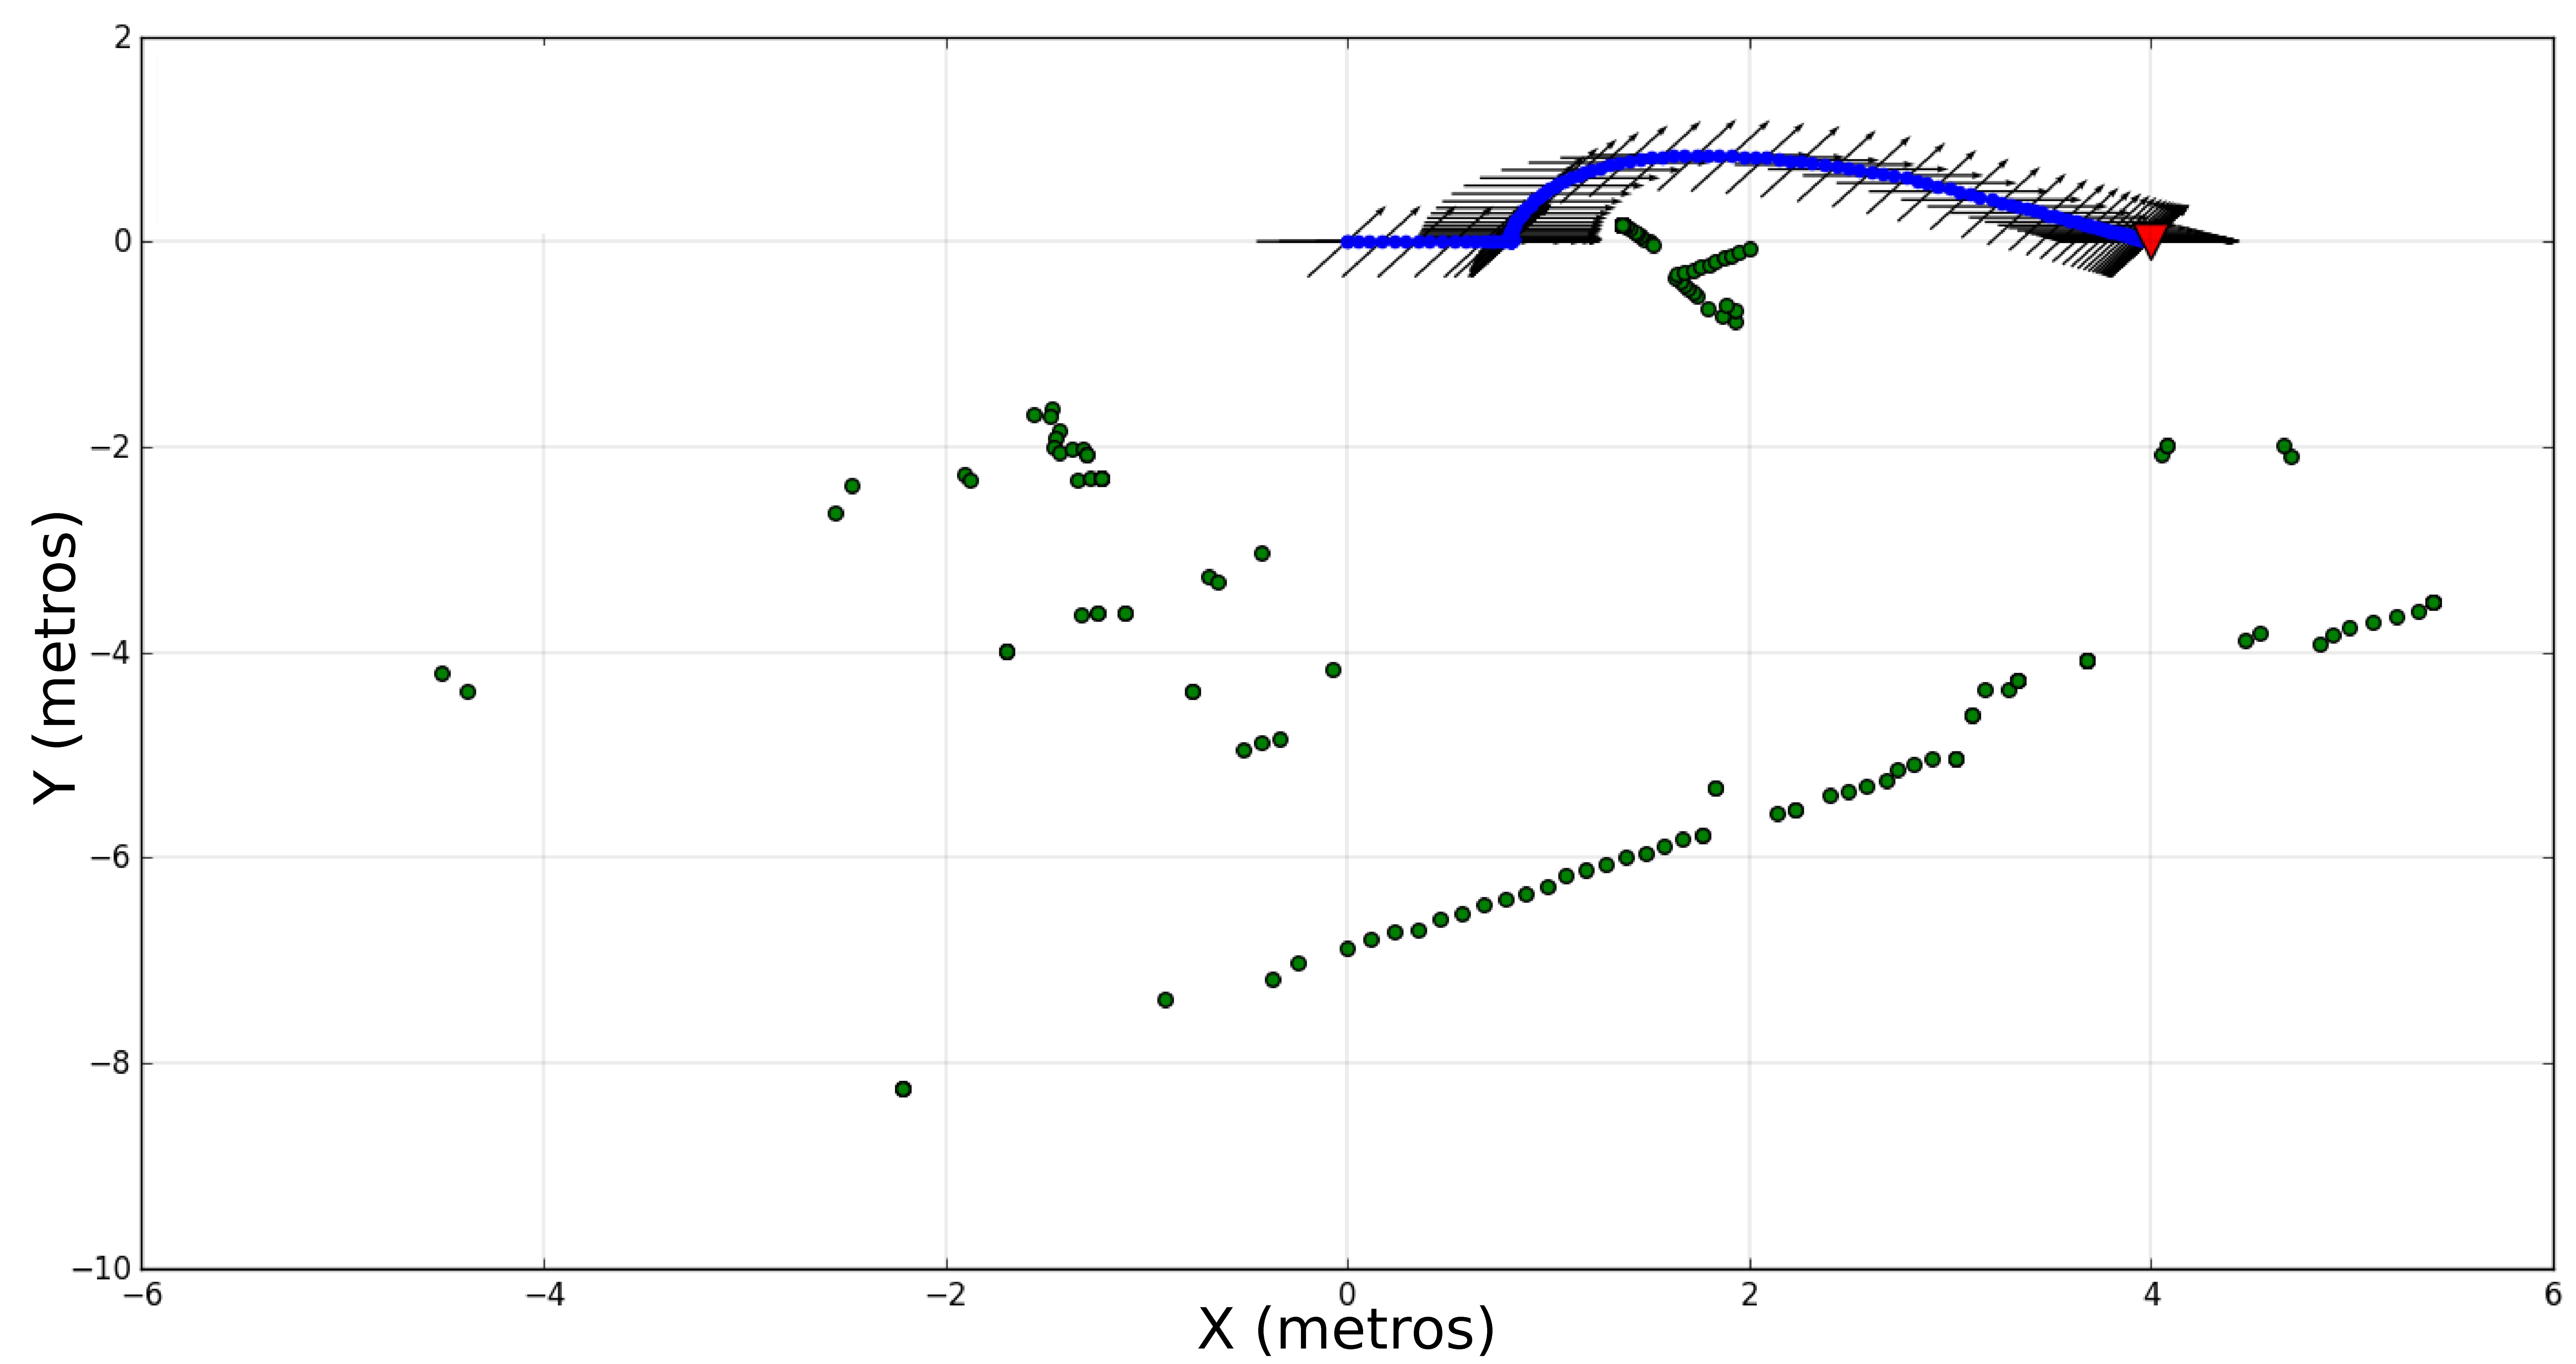
\includegraphics[width=.75\textwidth]{images/fnav_lidar_s.eps}}\\
      \multicolumn{1}{c}{(c)}
    \end{tabular}
  \captionsetup{font=footnotesize}
    \caption{\label{f:kbki_autonomo}Campos atractivos y repulsivos, y la trayectoria que el 
    robot real sigue usando datos en línea provenientes del sensor lídar montado en la parte 
    superior. En (a) se muestra las fuerzas de atracción, en (b) las fuerzas de repulsión y 
    las posiciones de los obsáculos, finalmente en (c) se muestra las fuerzas de navegación 
    generando la trayectoria.}
\end{figure}

%\begin{figure}%[ht!]
%  \centering \footnotesize
%  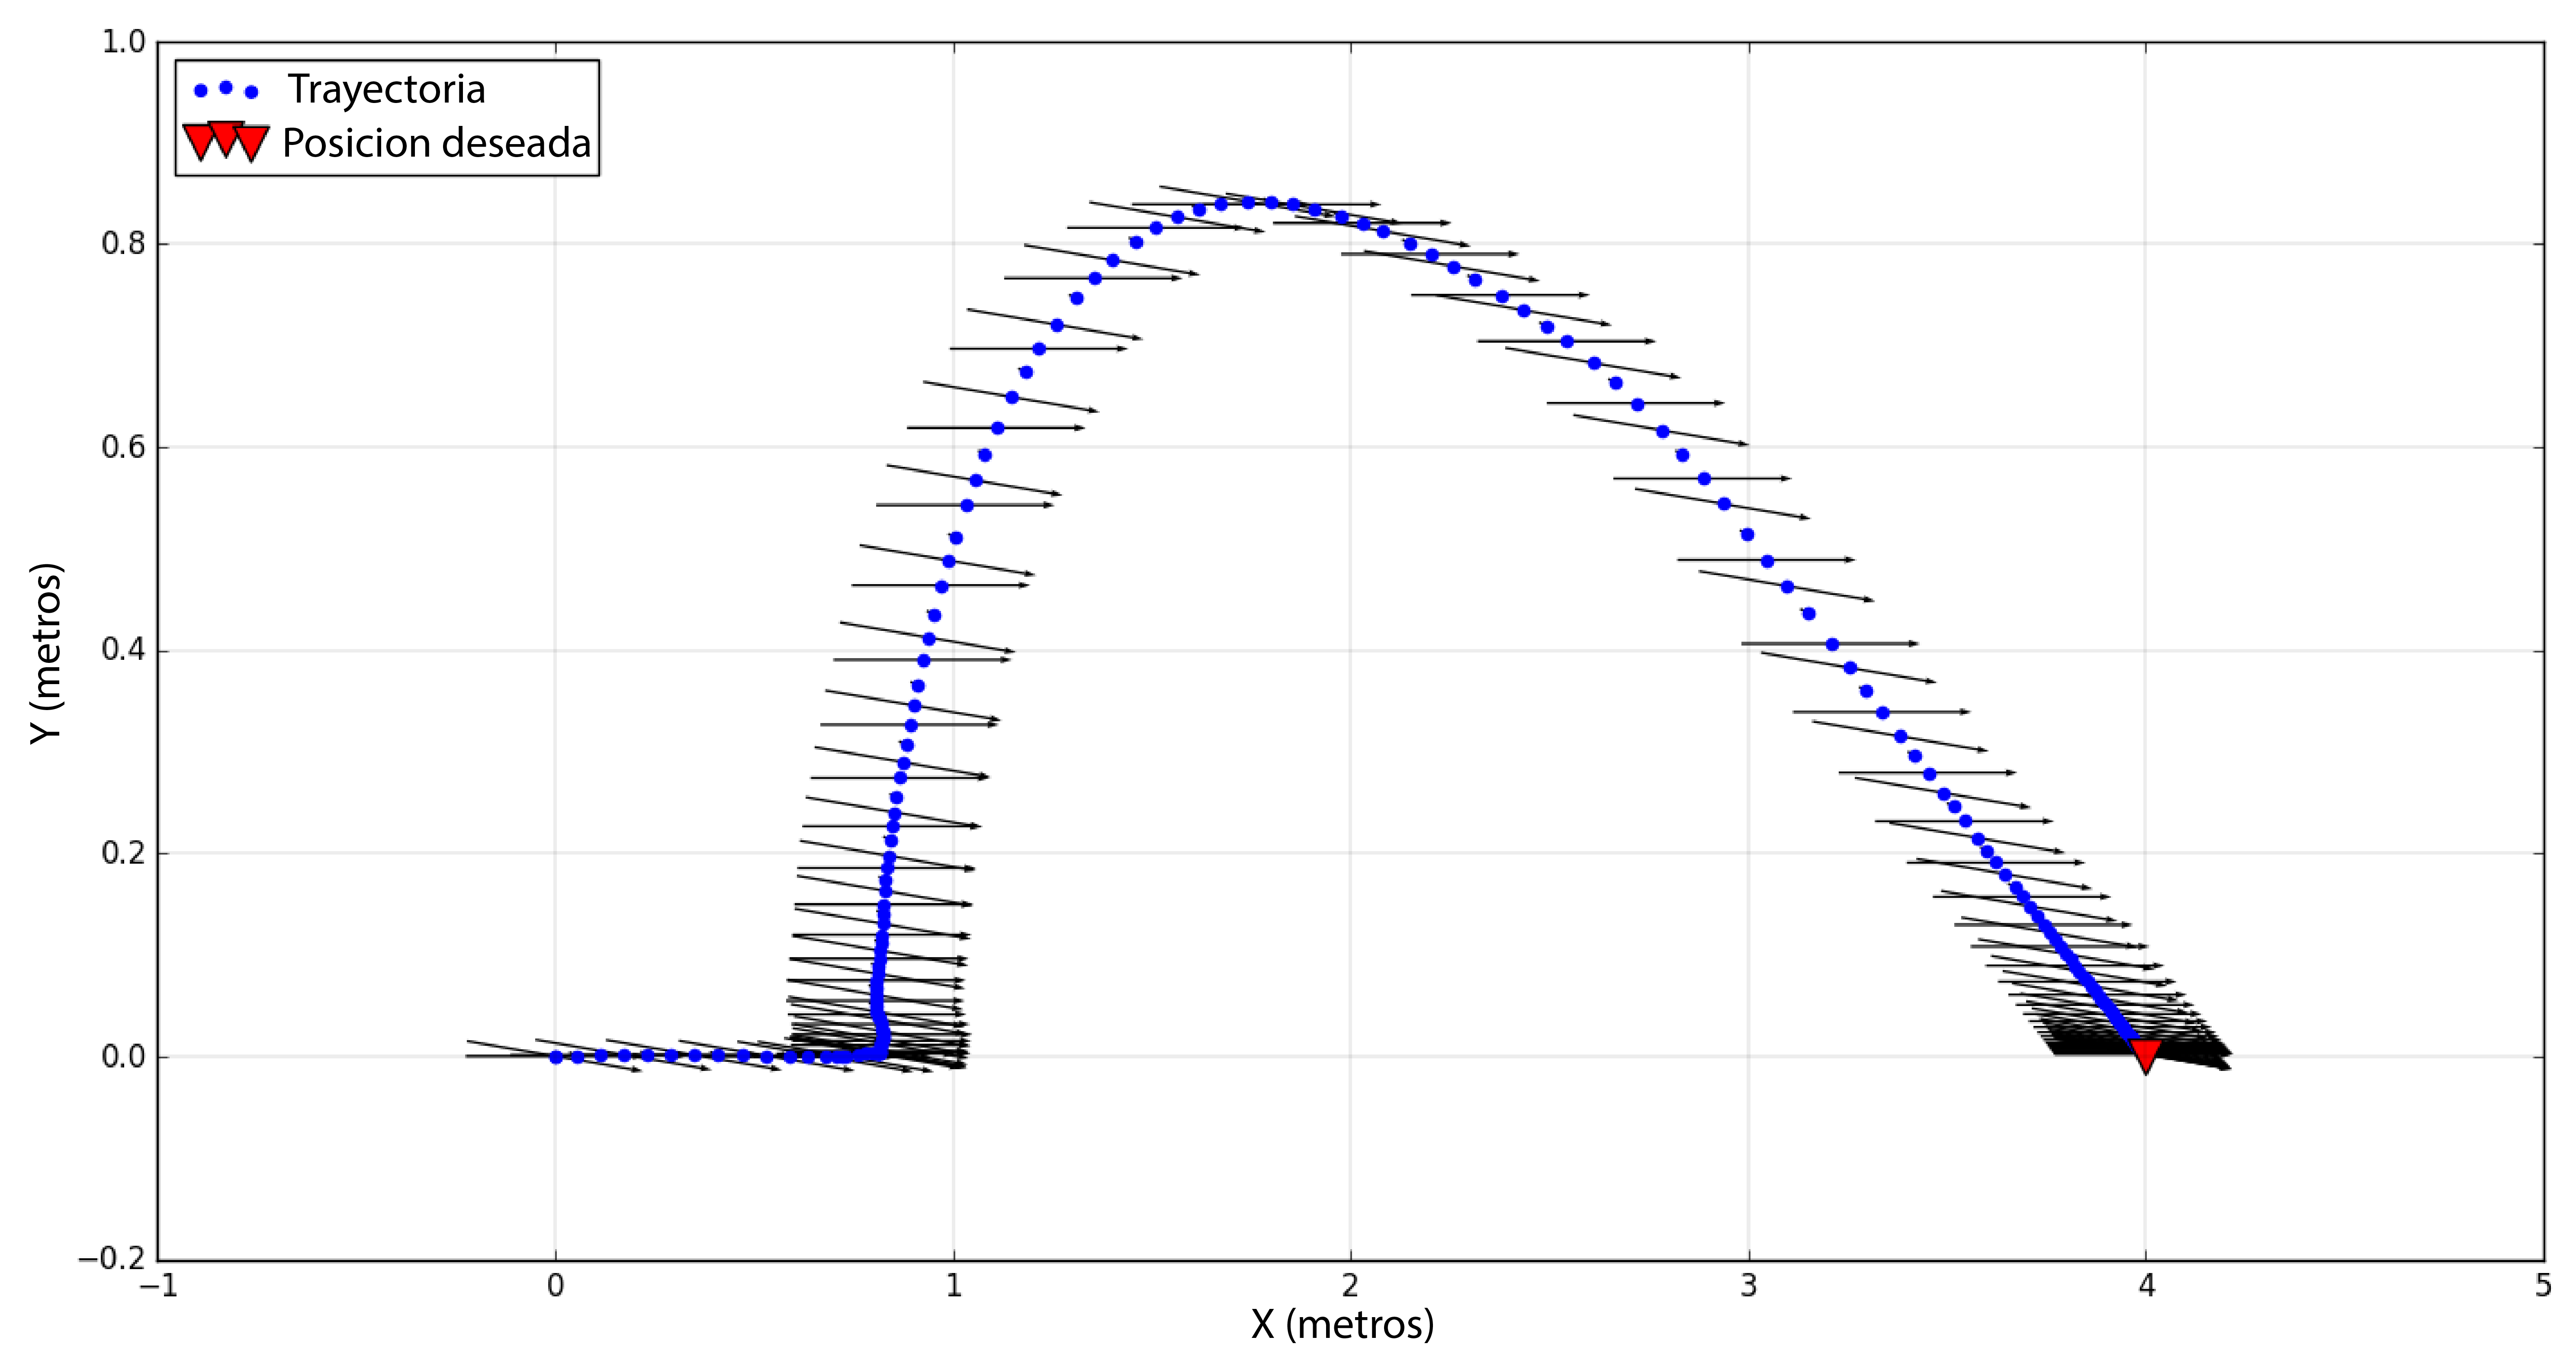
\includegraphics[width=0.80\textwidth]{images/fattr_lidar_s.png}
%  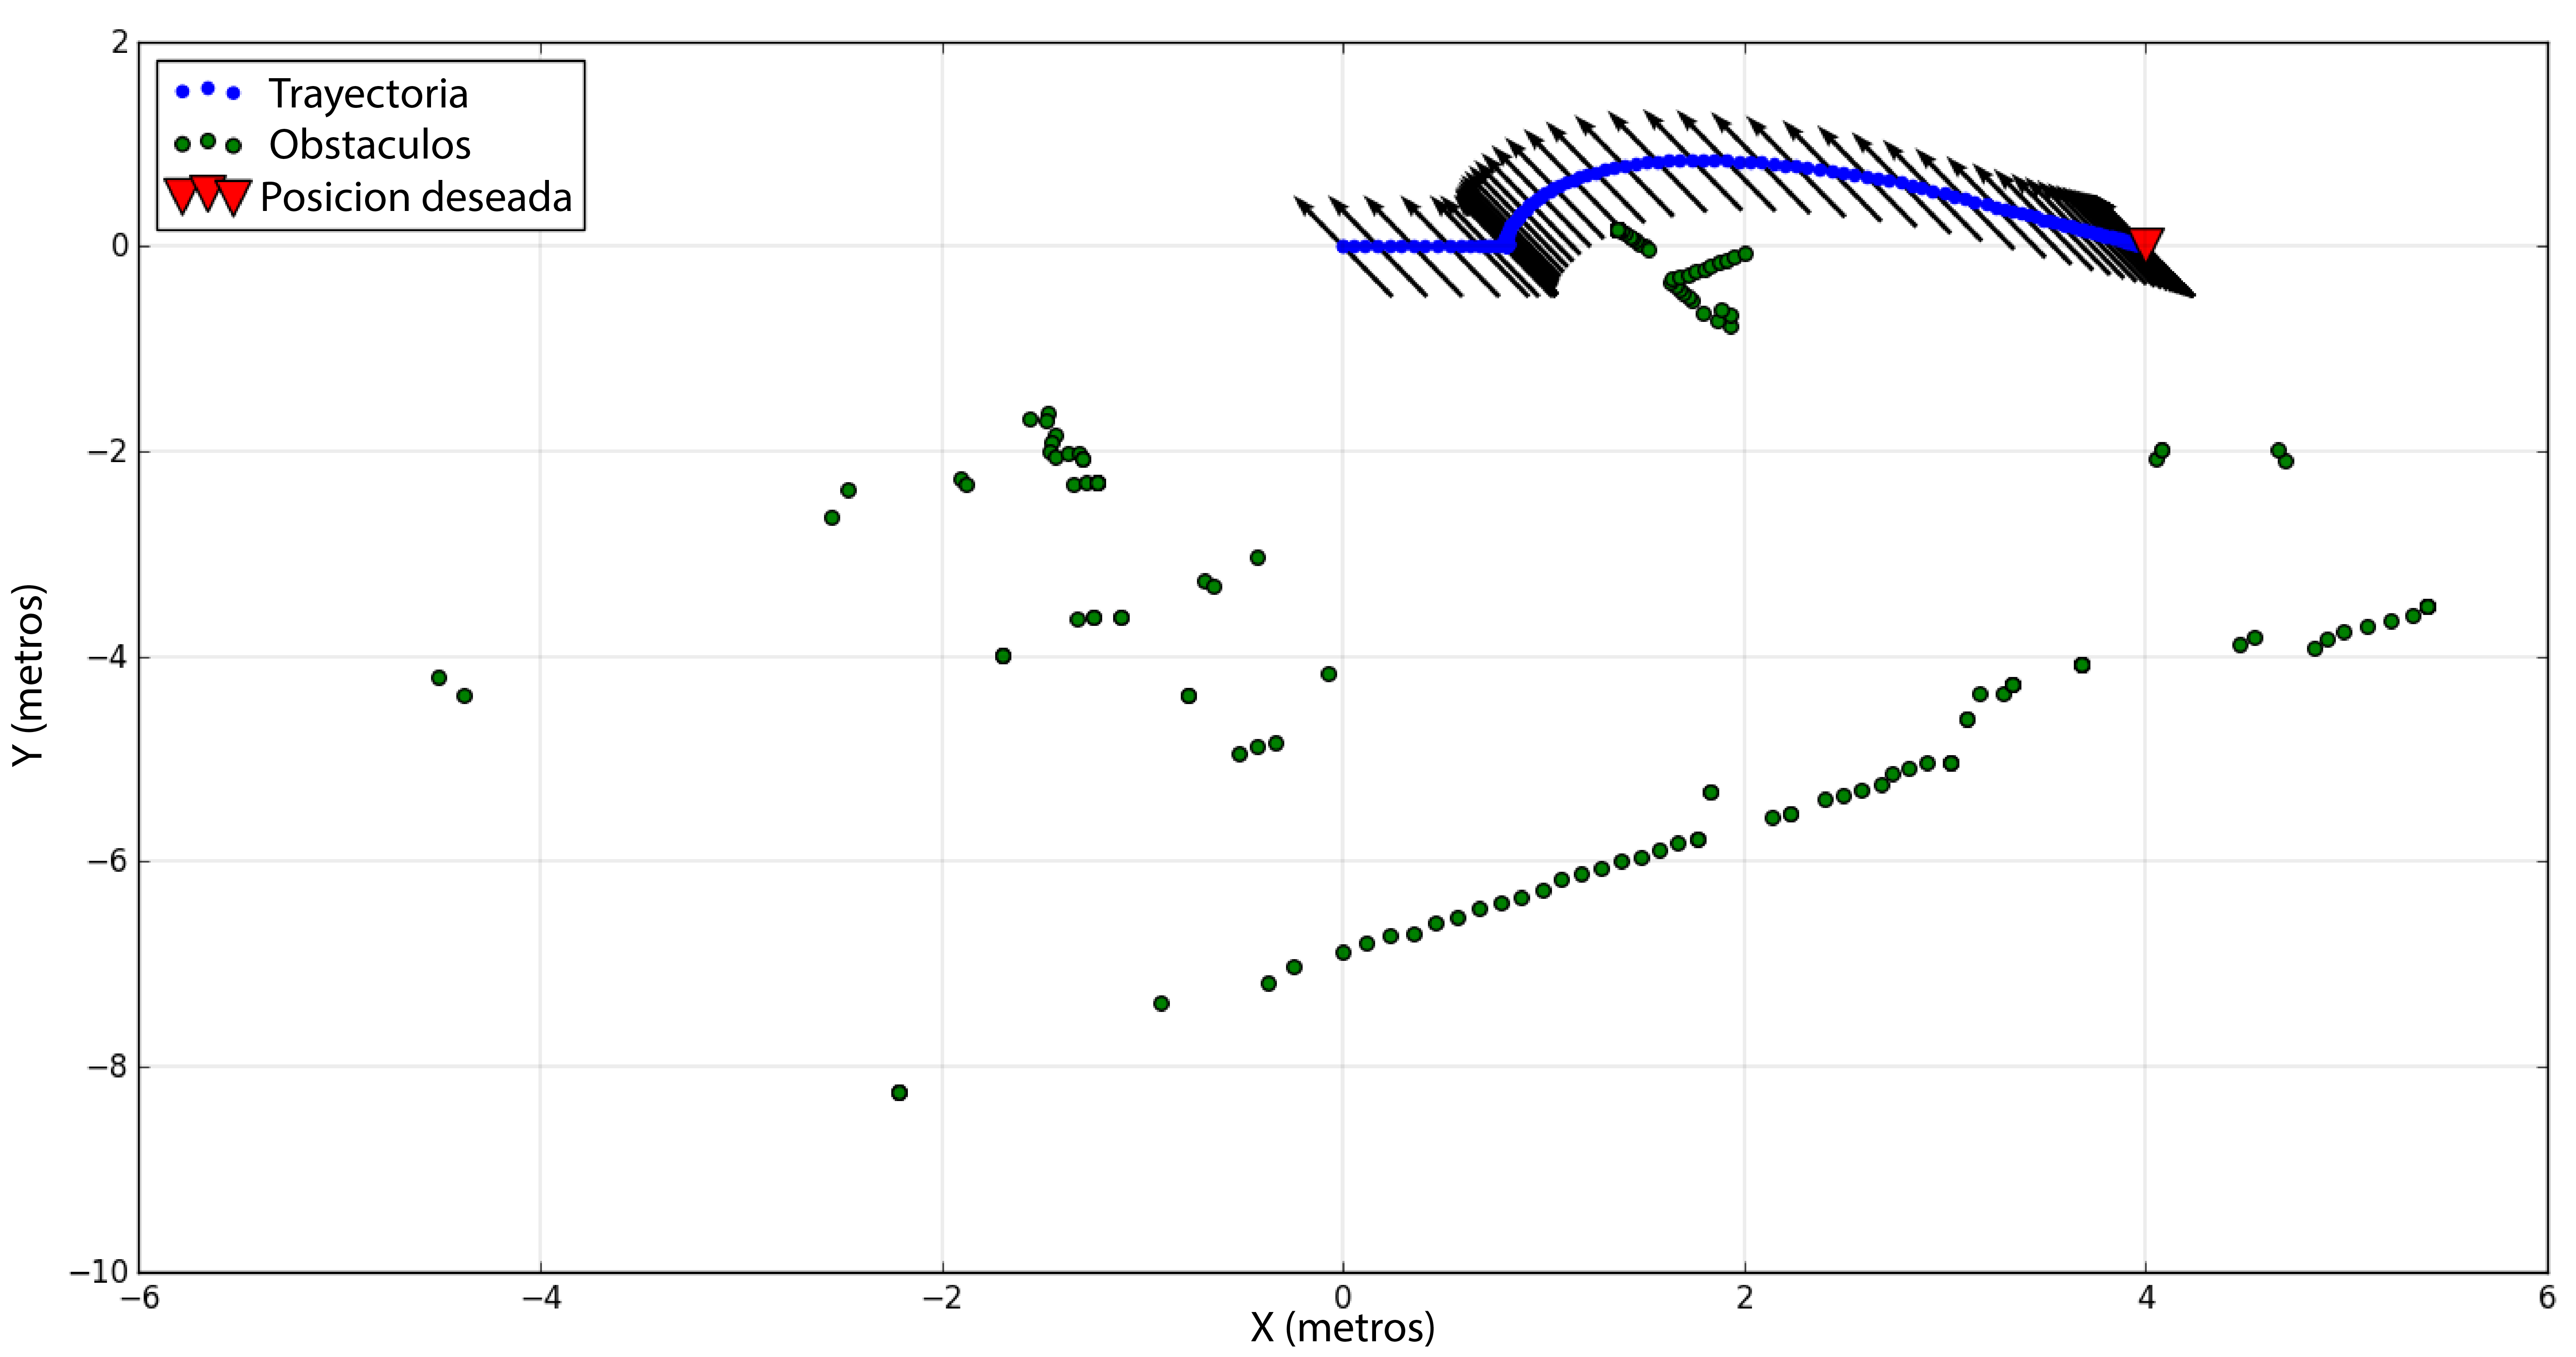
\includegraphics[width=0.80\textwidth]{images/frep_lidar_s.png}
%  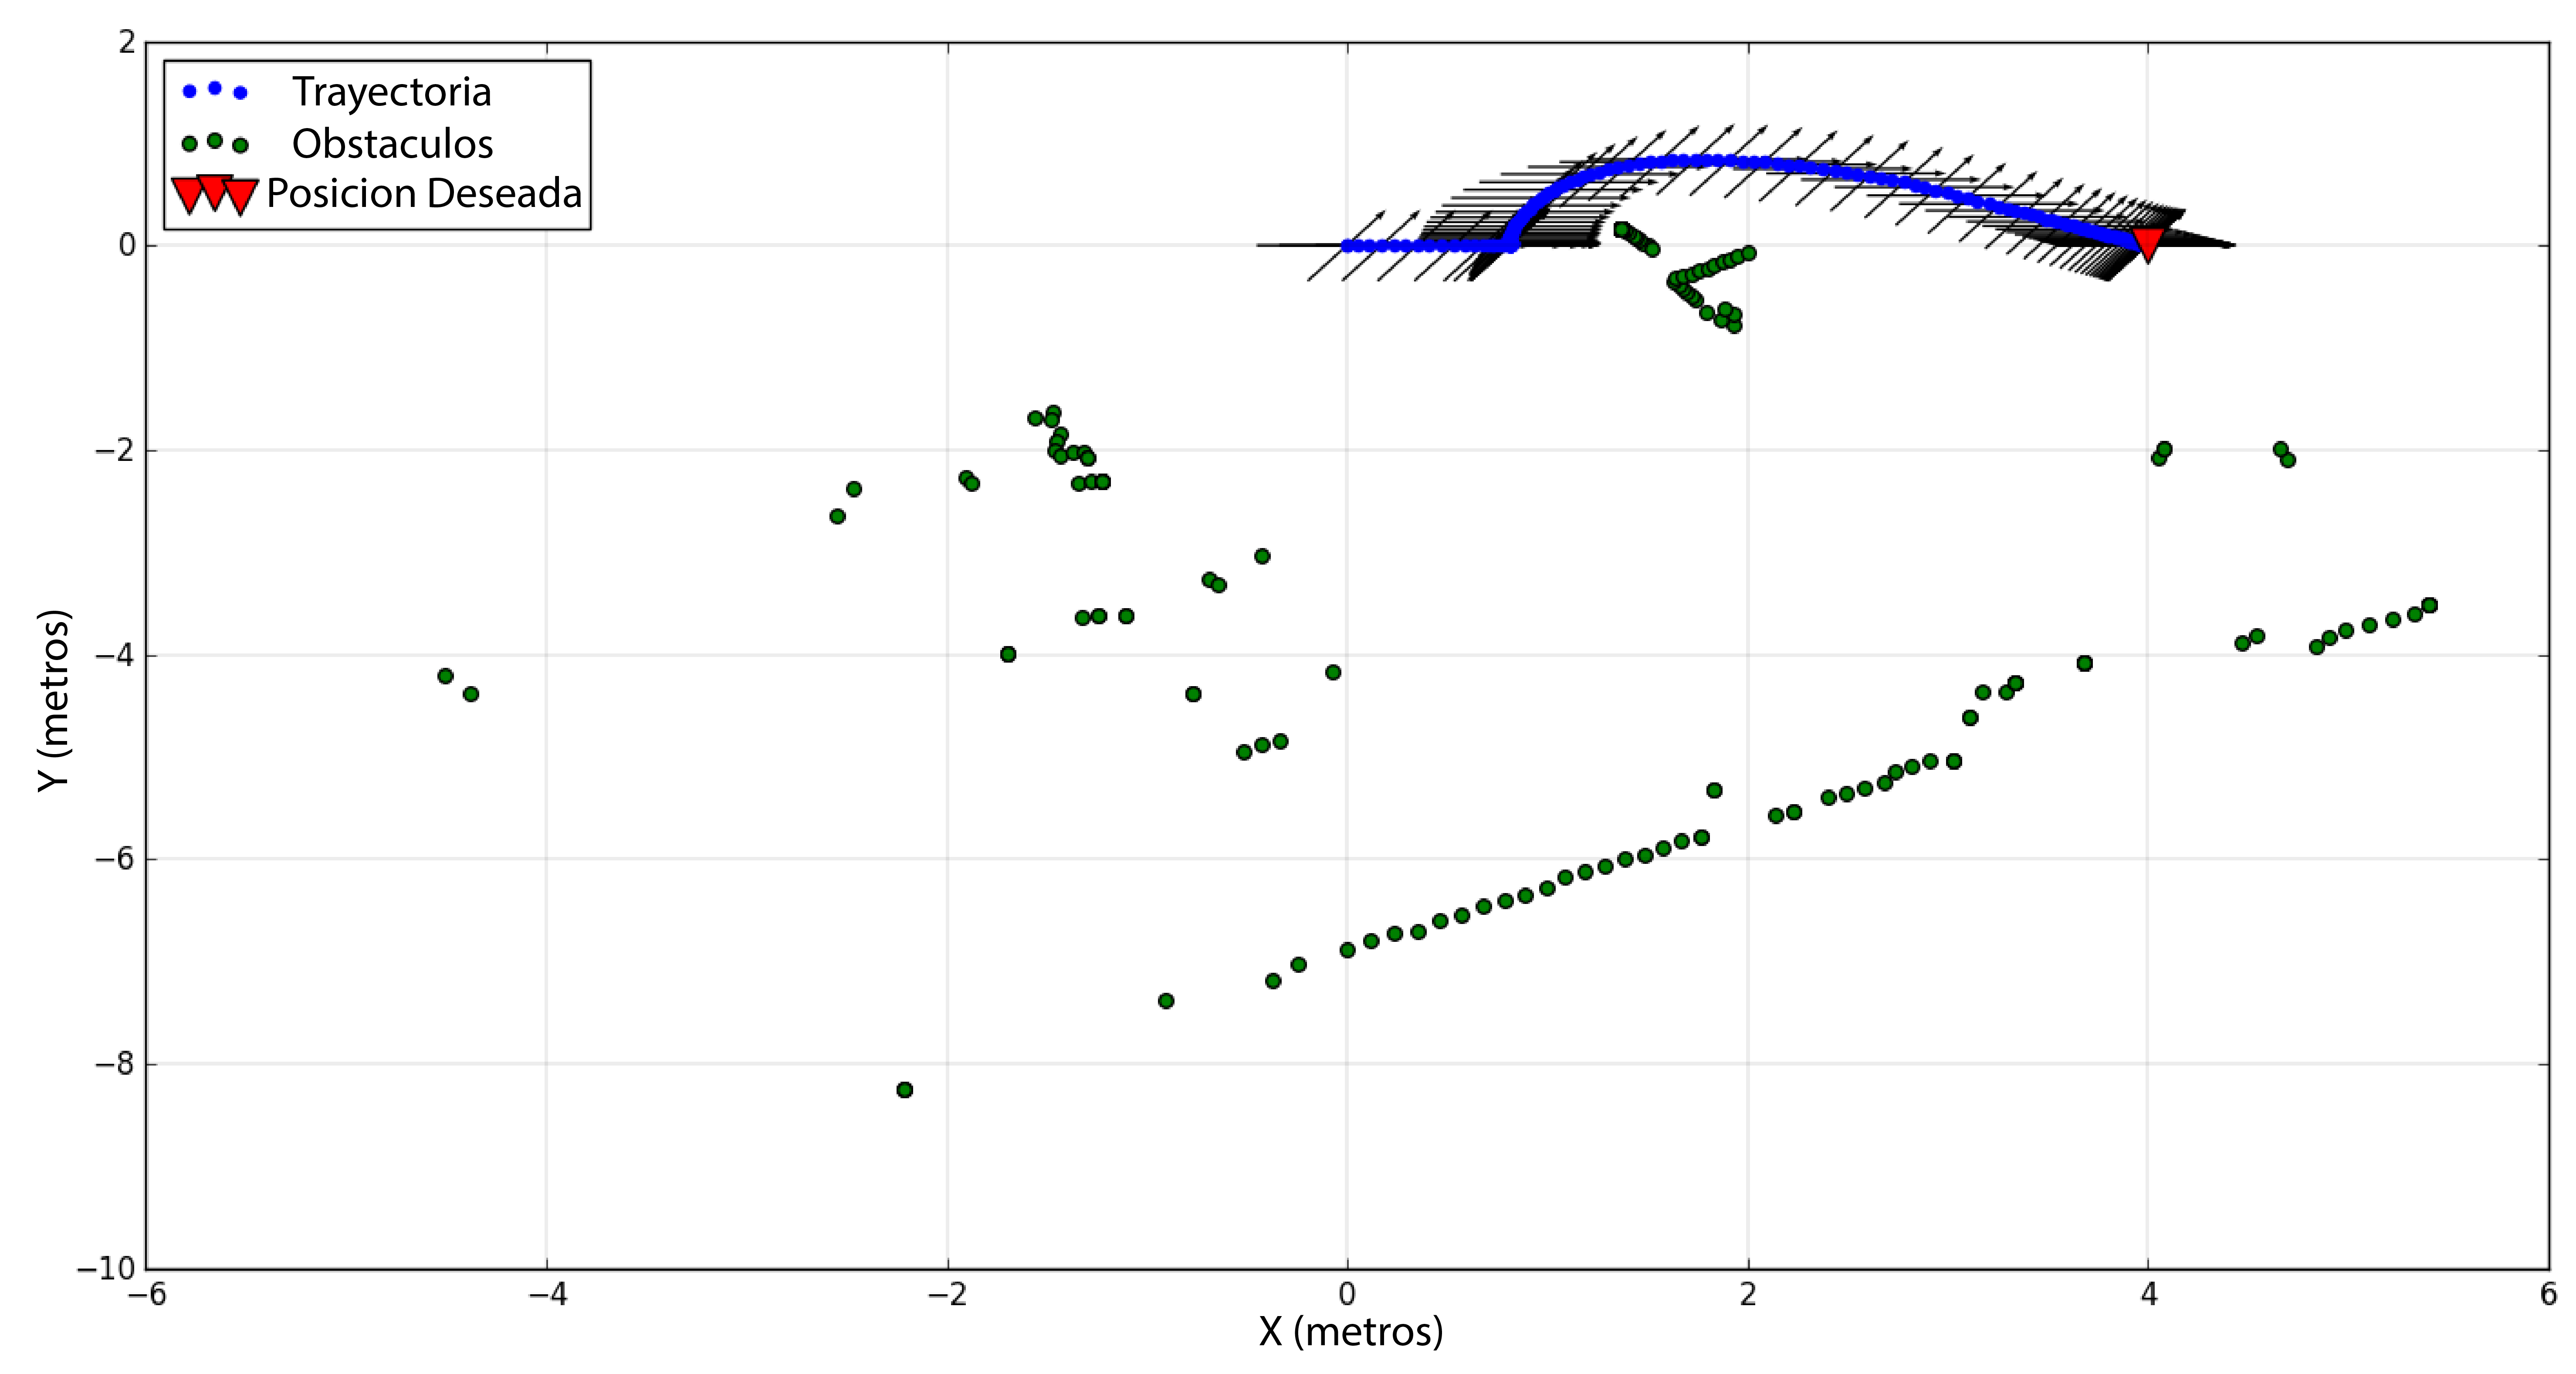
\includegraphics[width=0.80\textwidth]{images/fnav_lidar_s.png}
%  \captionsetup{font=footnotesize}
%  \caption{Campos atractivos y repulsivos, y la trayectoria que el robot real sigue 
%  usando datos en línea provenientes del sensor lidar montado en la parte superior.}
%  \label{f:kbki_autonomo}
%\end{figure}

Para probar la autonomía del robot móvil en un entorno real, se usa un sensor lídar 
(RPLidar A2) que se colocó sobre el robot Kobuki. Se usa el sensor lídar para poder 
hacer una actualización continua de las posiciones de los obstáculos a medida que el 
robot se mueve. El robot usa tópicos creados en ROS para obtener la información del 
sensor que se compone del rango y la orientación de cada punto medido, a medida que 
el lídar gira. La información del lídar se tuvo que convertir a coordenadas cartesianas 
para conocer las posiciones cartesianas de los obstáculos dentro del espacio de trabajo, 
que es la entrada al algoritmo principal. Para que el kobuki pueda moverse dentro del 
mapa generado por el lídar, el marco de referencia del robot se tomó como el marco del 
lídar. Entonces, el algoritmo de navegación autónomo usa las coordenadas del obstáculo 
para generar su propia trayectoria evitando obstáculos. Para toda la prueba, se colocaron 
dos cajas en el espacio de trabajo, como se ve en la Figura \ref{fig:Kobuki201}. La 
posición del objetivo era ($x = 4, y = 0$). La Figura \ref{f:kbki_autonomo}a muestra 
la trayectoria del robot en azul y las flechas que indican la fuerza que lleva al robot a la 
posición deseada. La Figura \ref{f:kbki_autonomo}b muestra el mapa completo, donde los 
puntos verdes representan el entorno, detectados por el lídar, donde se mueve el robot. Como 
se observa, estas flechas apuntan hacia afuera del obstáculo, proporcionando autonomía al 
robot mientras intenta alcanzar la posición deseada. Finalmente en la Figura 
\ref{f:kbki_autonomo}c se muestra toda la fuerza de navegación que impulsa el movimiento 
del robot móvil.

\section{Resultado de la Navegación Autónoma usando SLAM en dos dimensiones}
\begin{figure}%[ht!]
  \centering \footnotesize
  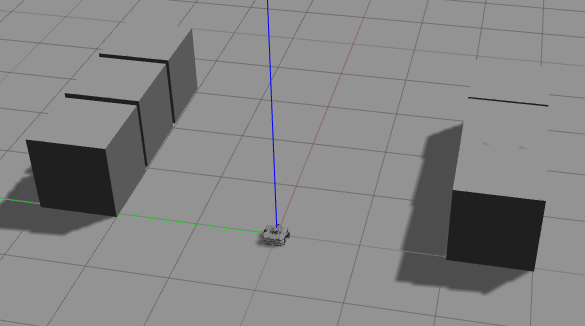
\includegraphics[width=0.80\textwidth]{images/gazebo_map.png}
  \captionsetup{font=footnotesize}
  \caption{Robot móvil Kobuki en medio de los obstáculos colocados para probar la 
  navegación autónoma utilizando el algoritmo SLAM. Esta prueba se realizó en el
  simulador Gazebo.}
  \label{fig:Gazebo_simu}
\end{figure}
Para probar la navegación autónoma del robot Kobuki usando el algoritmo SLAM, se utilizó
el simulador dinámico Gazebo. En este simulador se creó un escenario donde se colocó al 
robot Kobuki en medio de varios obstáculos. Los obstáculos fueron colocados de tal forma
que pueda representar la entrada de un túnel. En la Figura \ref{fig:Gazebo_simu} se puede
ver el escenario que fue creado. Un conjunto de obstáculos tiene una longitud de 3 metros
y el ancho entre los conjuntos de obstáculos es de 4 metros. El robot tiene que desplazarse
por ese espacio hasta llegar a la posición deseada, estimar la posición de los obstáculos 
y construir el mapa en dos dimensiones.

\begin{figure}%[ht!]
     %\begin{center}
     %   \subfigure[Fuerzas de atracción aplicado al robot móvil en tiempo real]{\label{fig:etiquetaA}\includegraphics
     %   [width=.69\textwidth]{images/fattr_slam.png}}
     %   \subfigure[Fuerzas de repulsión aplicado al robot móvil en tiempo real]{\label{fig:etiquetaB}\includegraphics
     %   [width=.69\textwidth]{images/frep_slam.png}}
     %   \subfigure[Fuerzas de navegación aplicado al robot móvil en tiempo real]{\label{fig:etiquetaC}\includegraphics
     %   [width=.69\textwidth]{images/fnav_slam.png}}
    %\end{center}
    \centering
    \begin{tabular}{c}
      \multicolumn{1}{c}{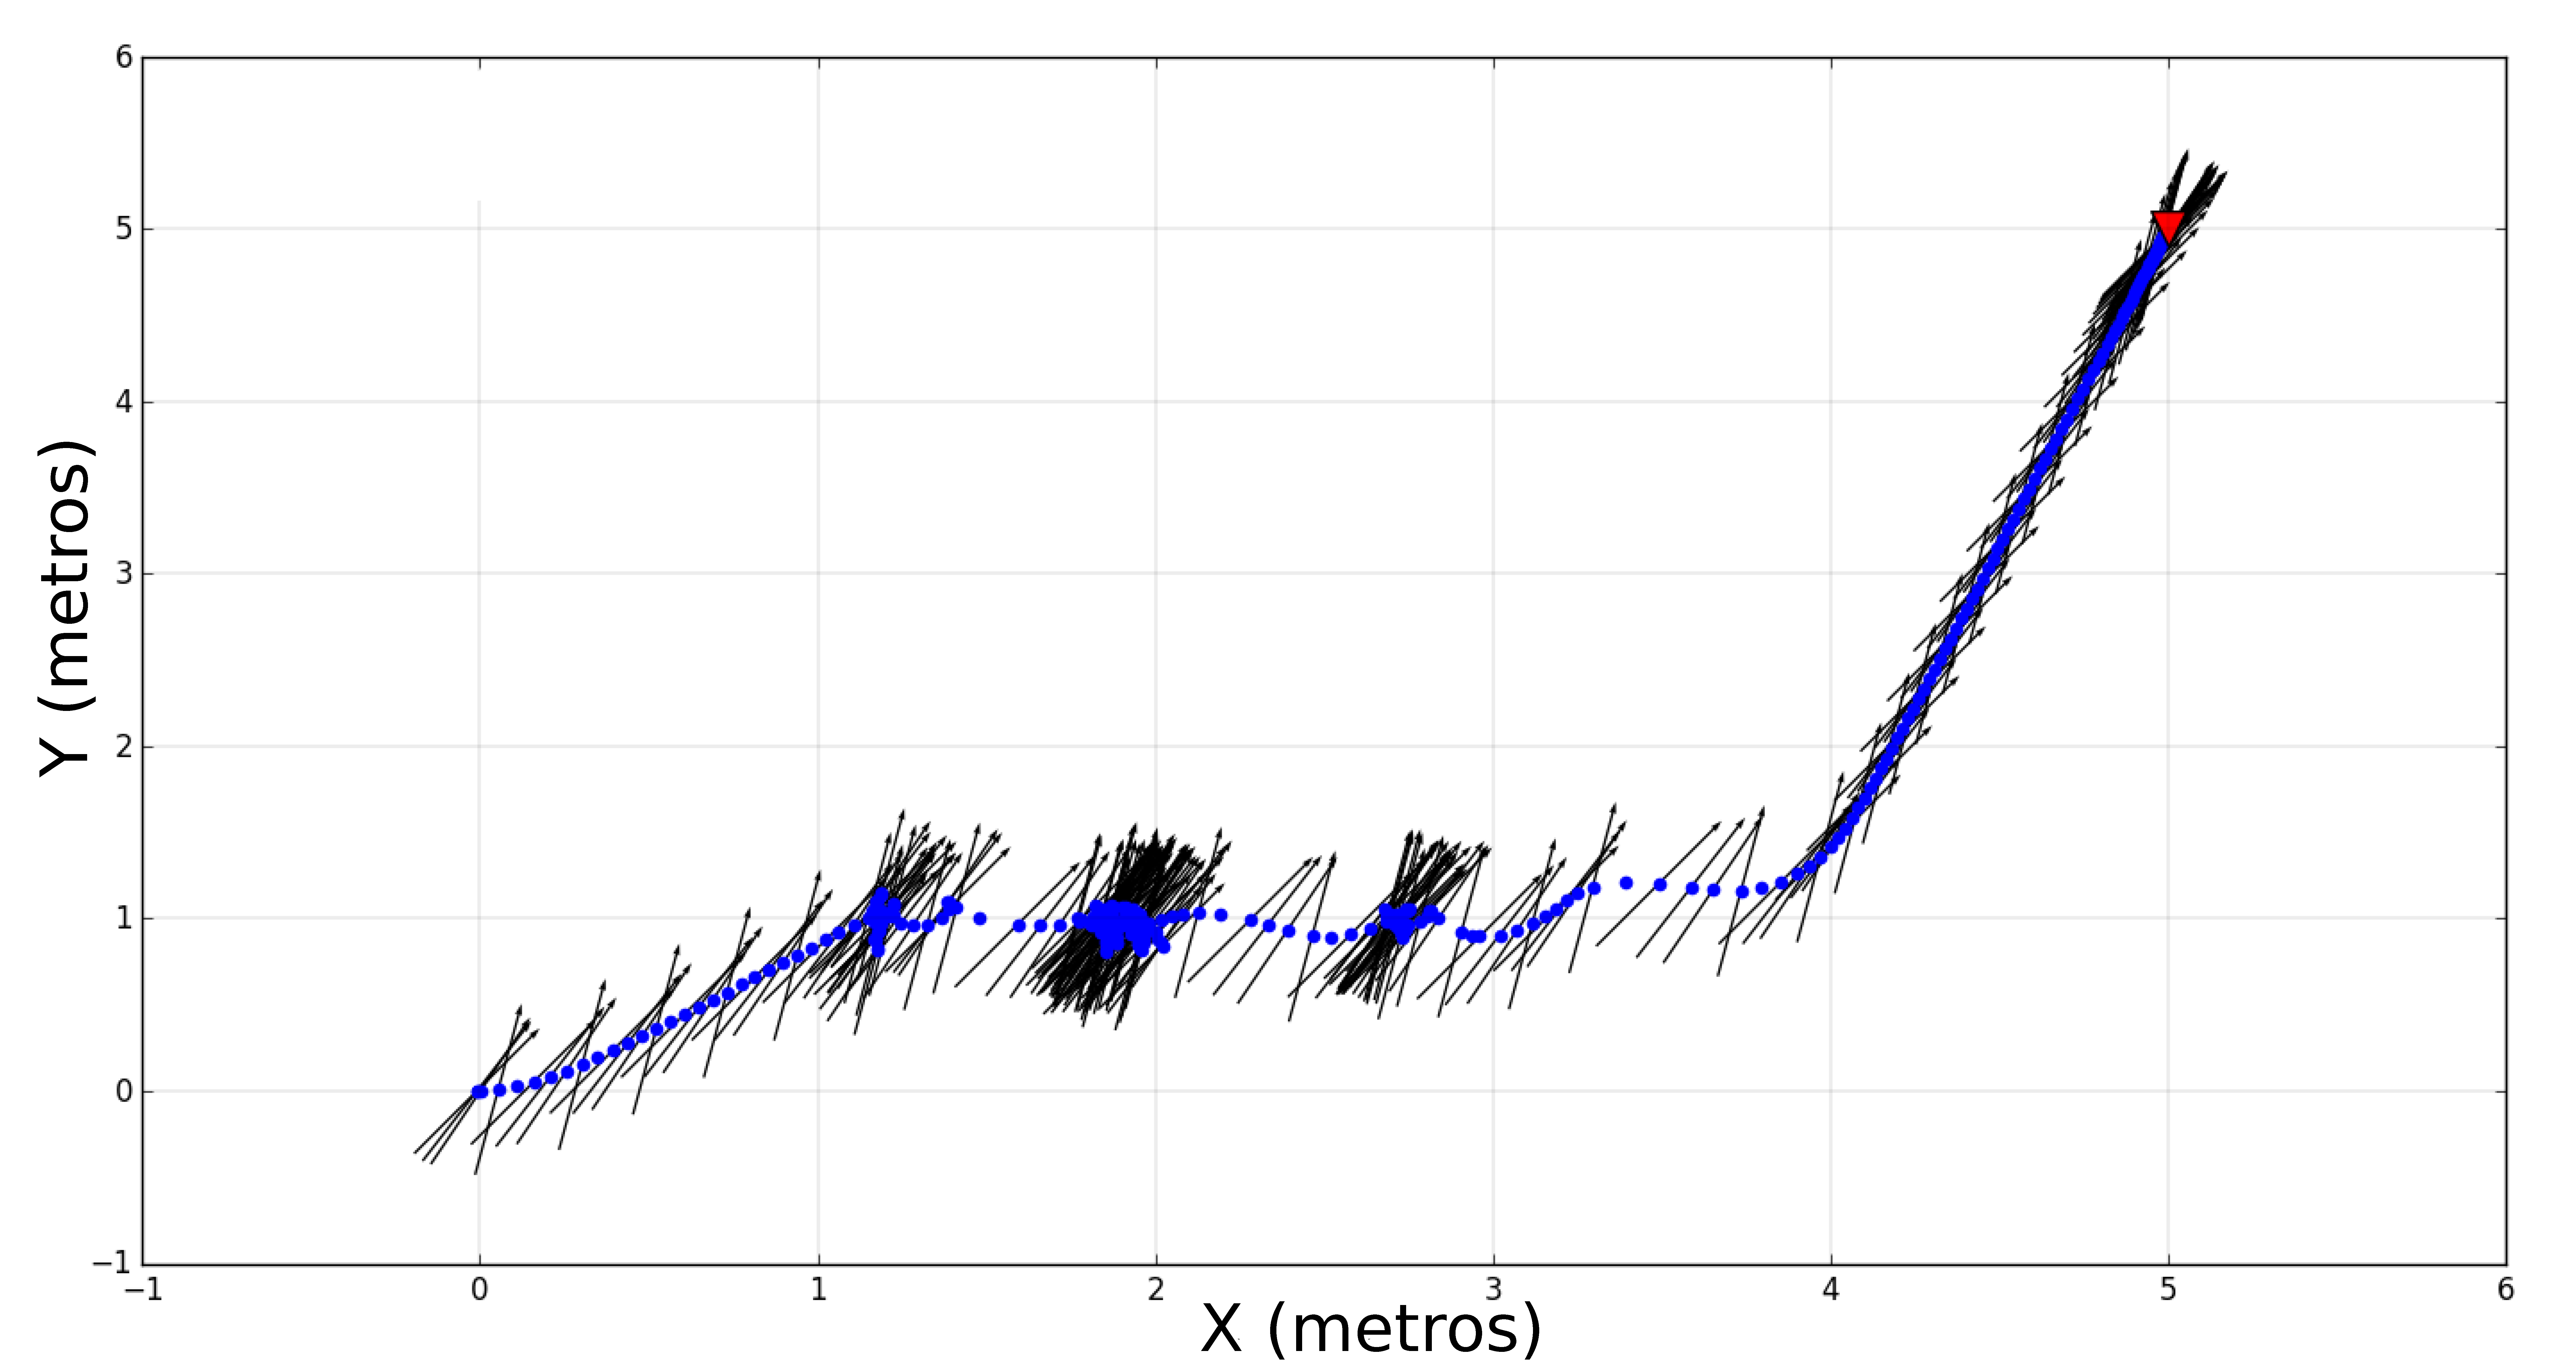
\includegraphics[width=.77\textwidth]{images/fattr_slam.eps}}\\
      \multicolumn{1}{c}{(a)}\\
      \multicolumn{1}{c}{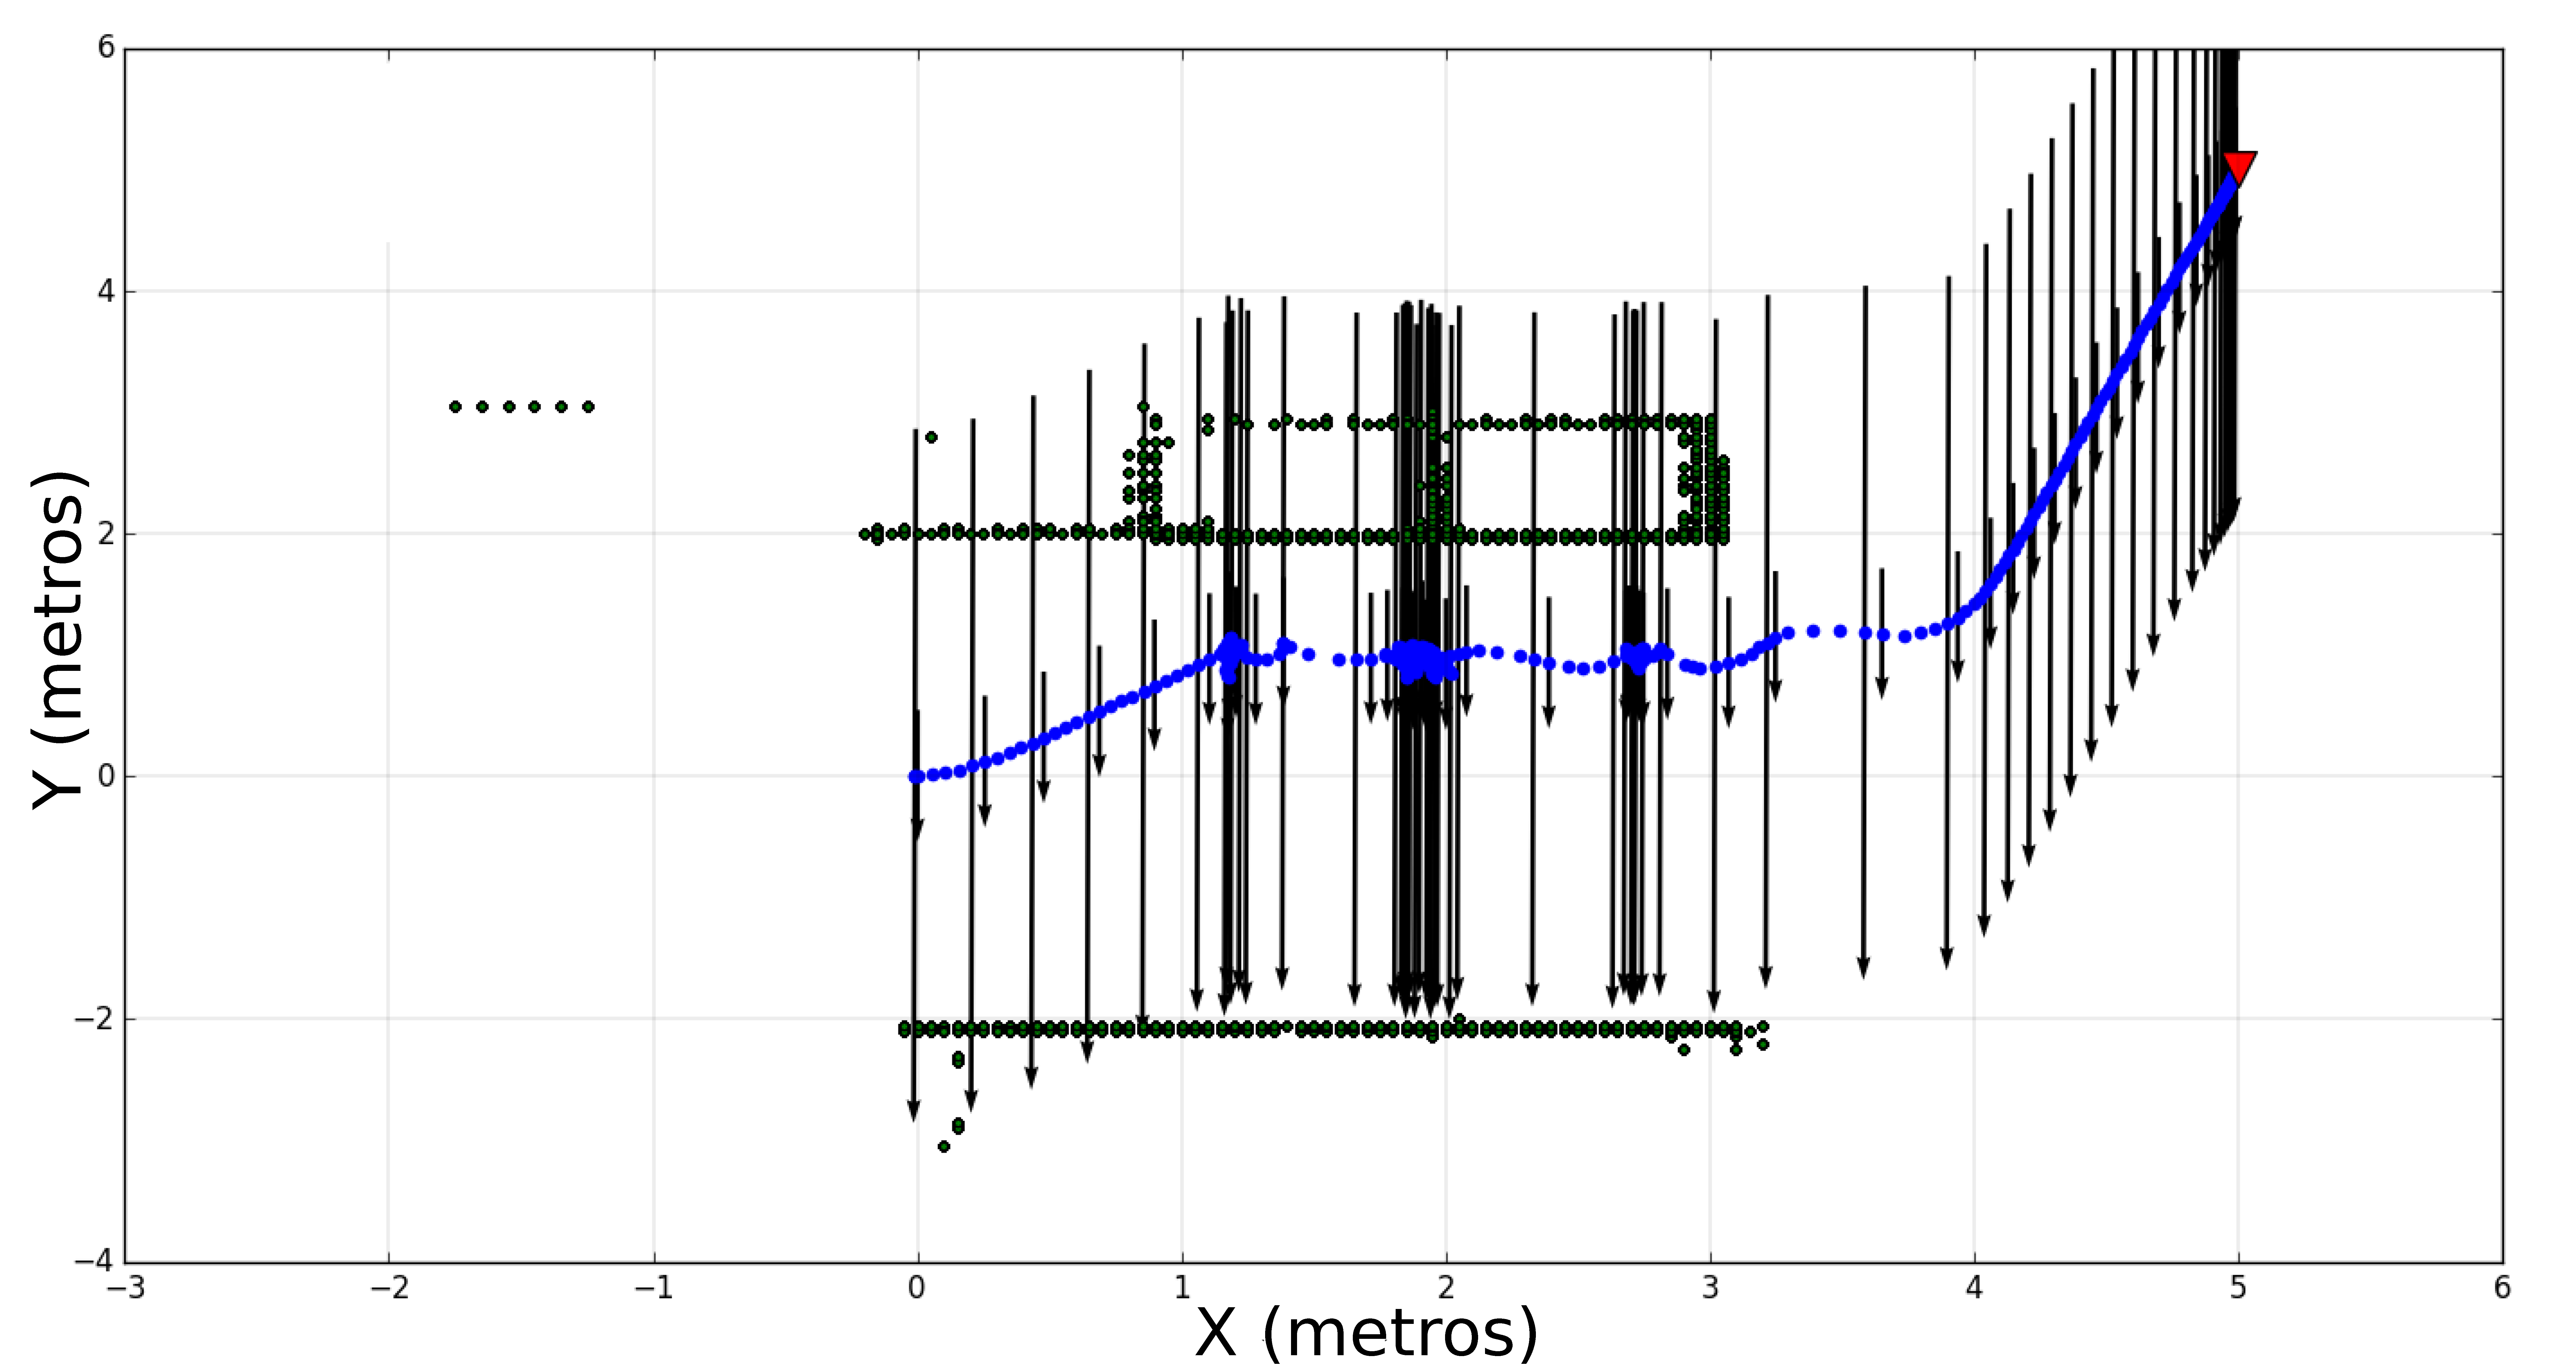
\includegraphics[width=.77\textwidth]{images/frep_slam.eps}}\\
      \multicolumn{1}{c}{(b)}\\
      \multicolumn{1}{c}{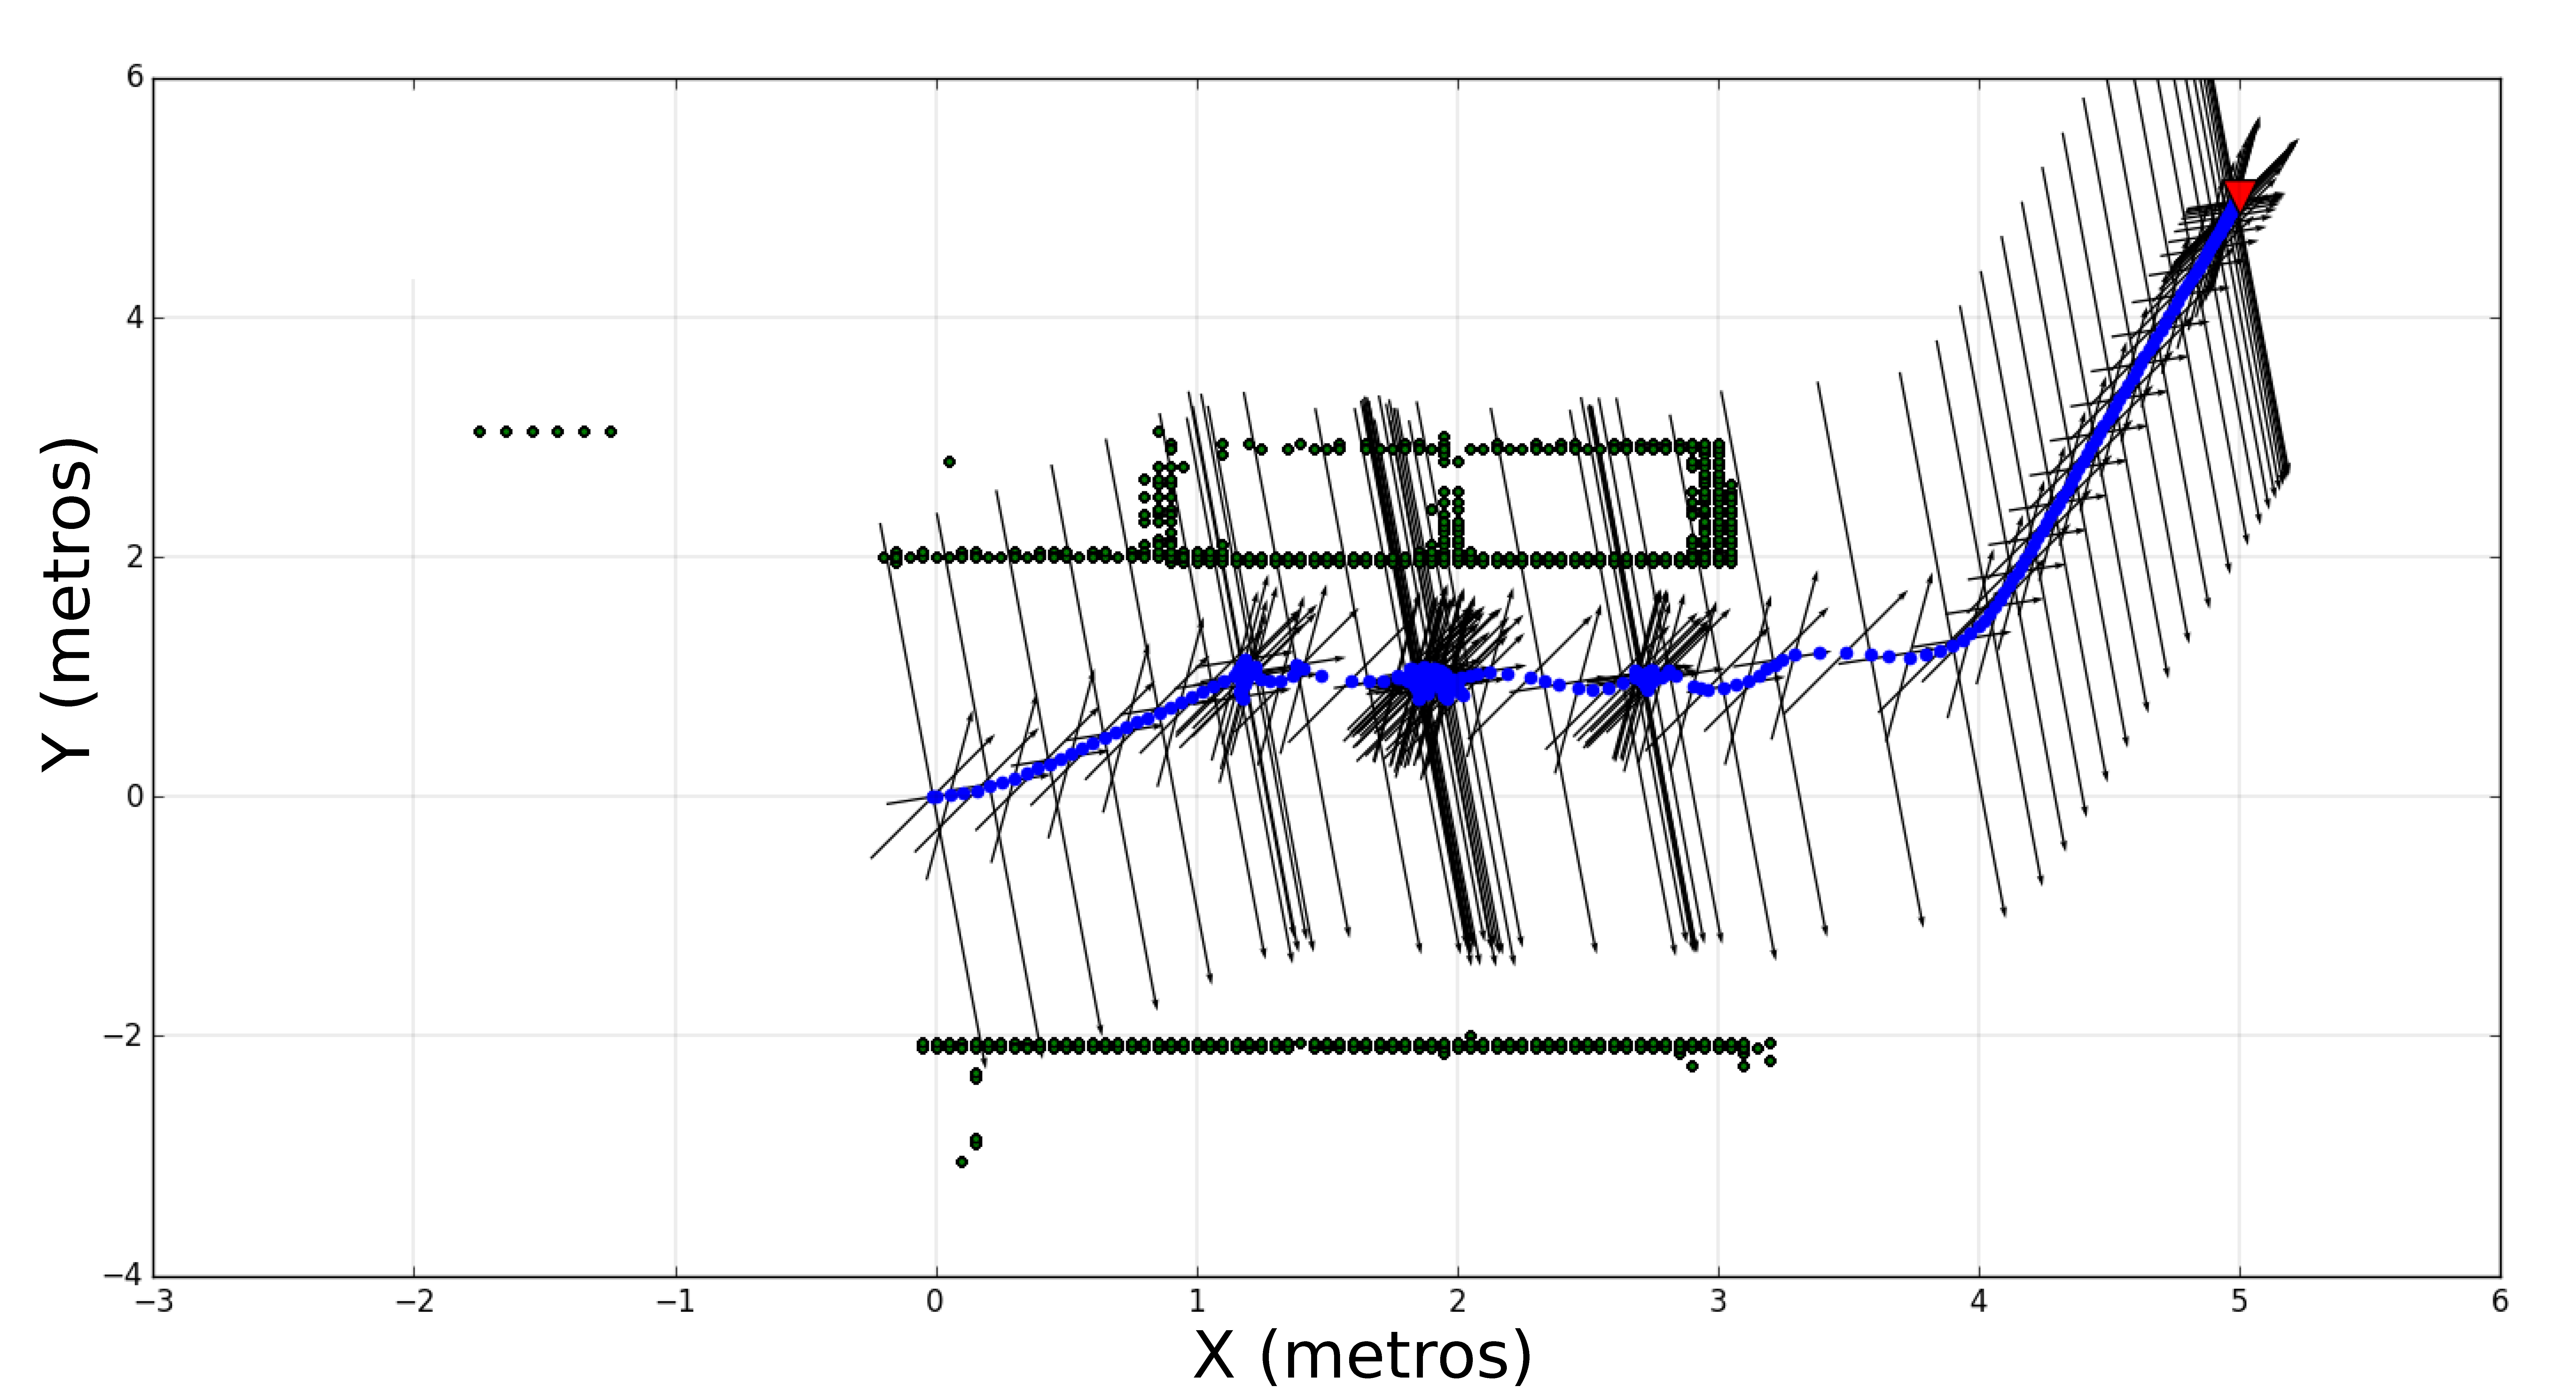
\includegraphics[width=.77\textwidth]{images/fnav_slam.eps}}\\
      \multicolumn{1}{c}{(c)}
    \end{tabular}
  \captionsetup{font=footnotesize}
    \caption{\label{fig:Kbki_slam}Navegación autónoma del Kobuki utilizando
    SLAM. En (a) se muestra las fuerzas de atracción, en (b) se representa 
    las fuerzas de repulsión y en (c) la suma de las fuerzas de atracción y 
    repulsión.}
\end{figure}

%\begin{figure}%[ht!]
%  \centering \footnotesize
%  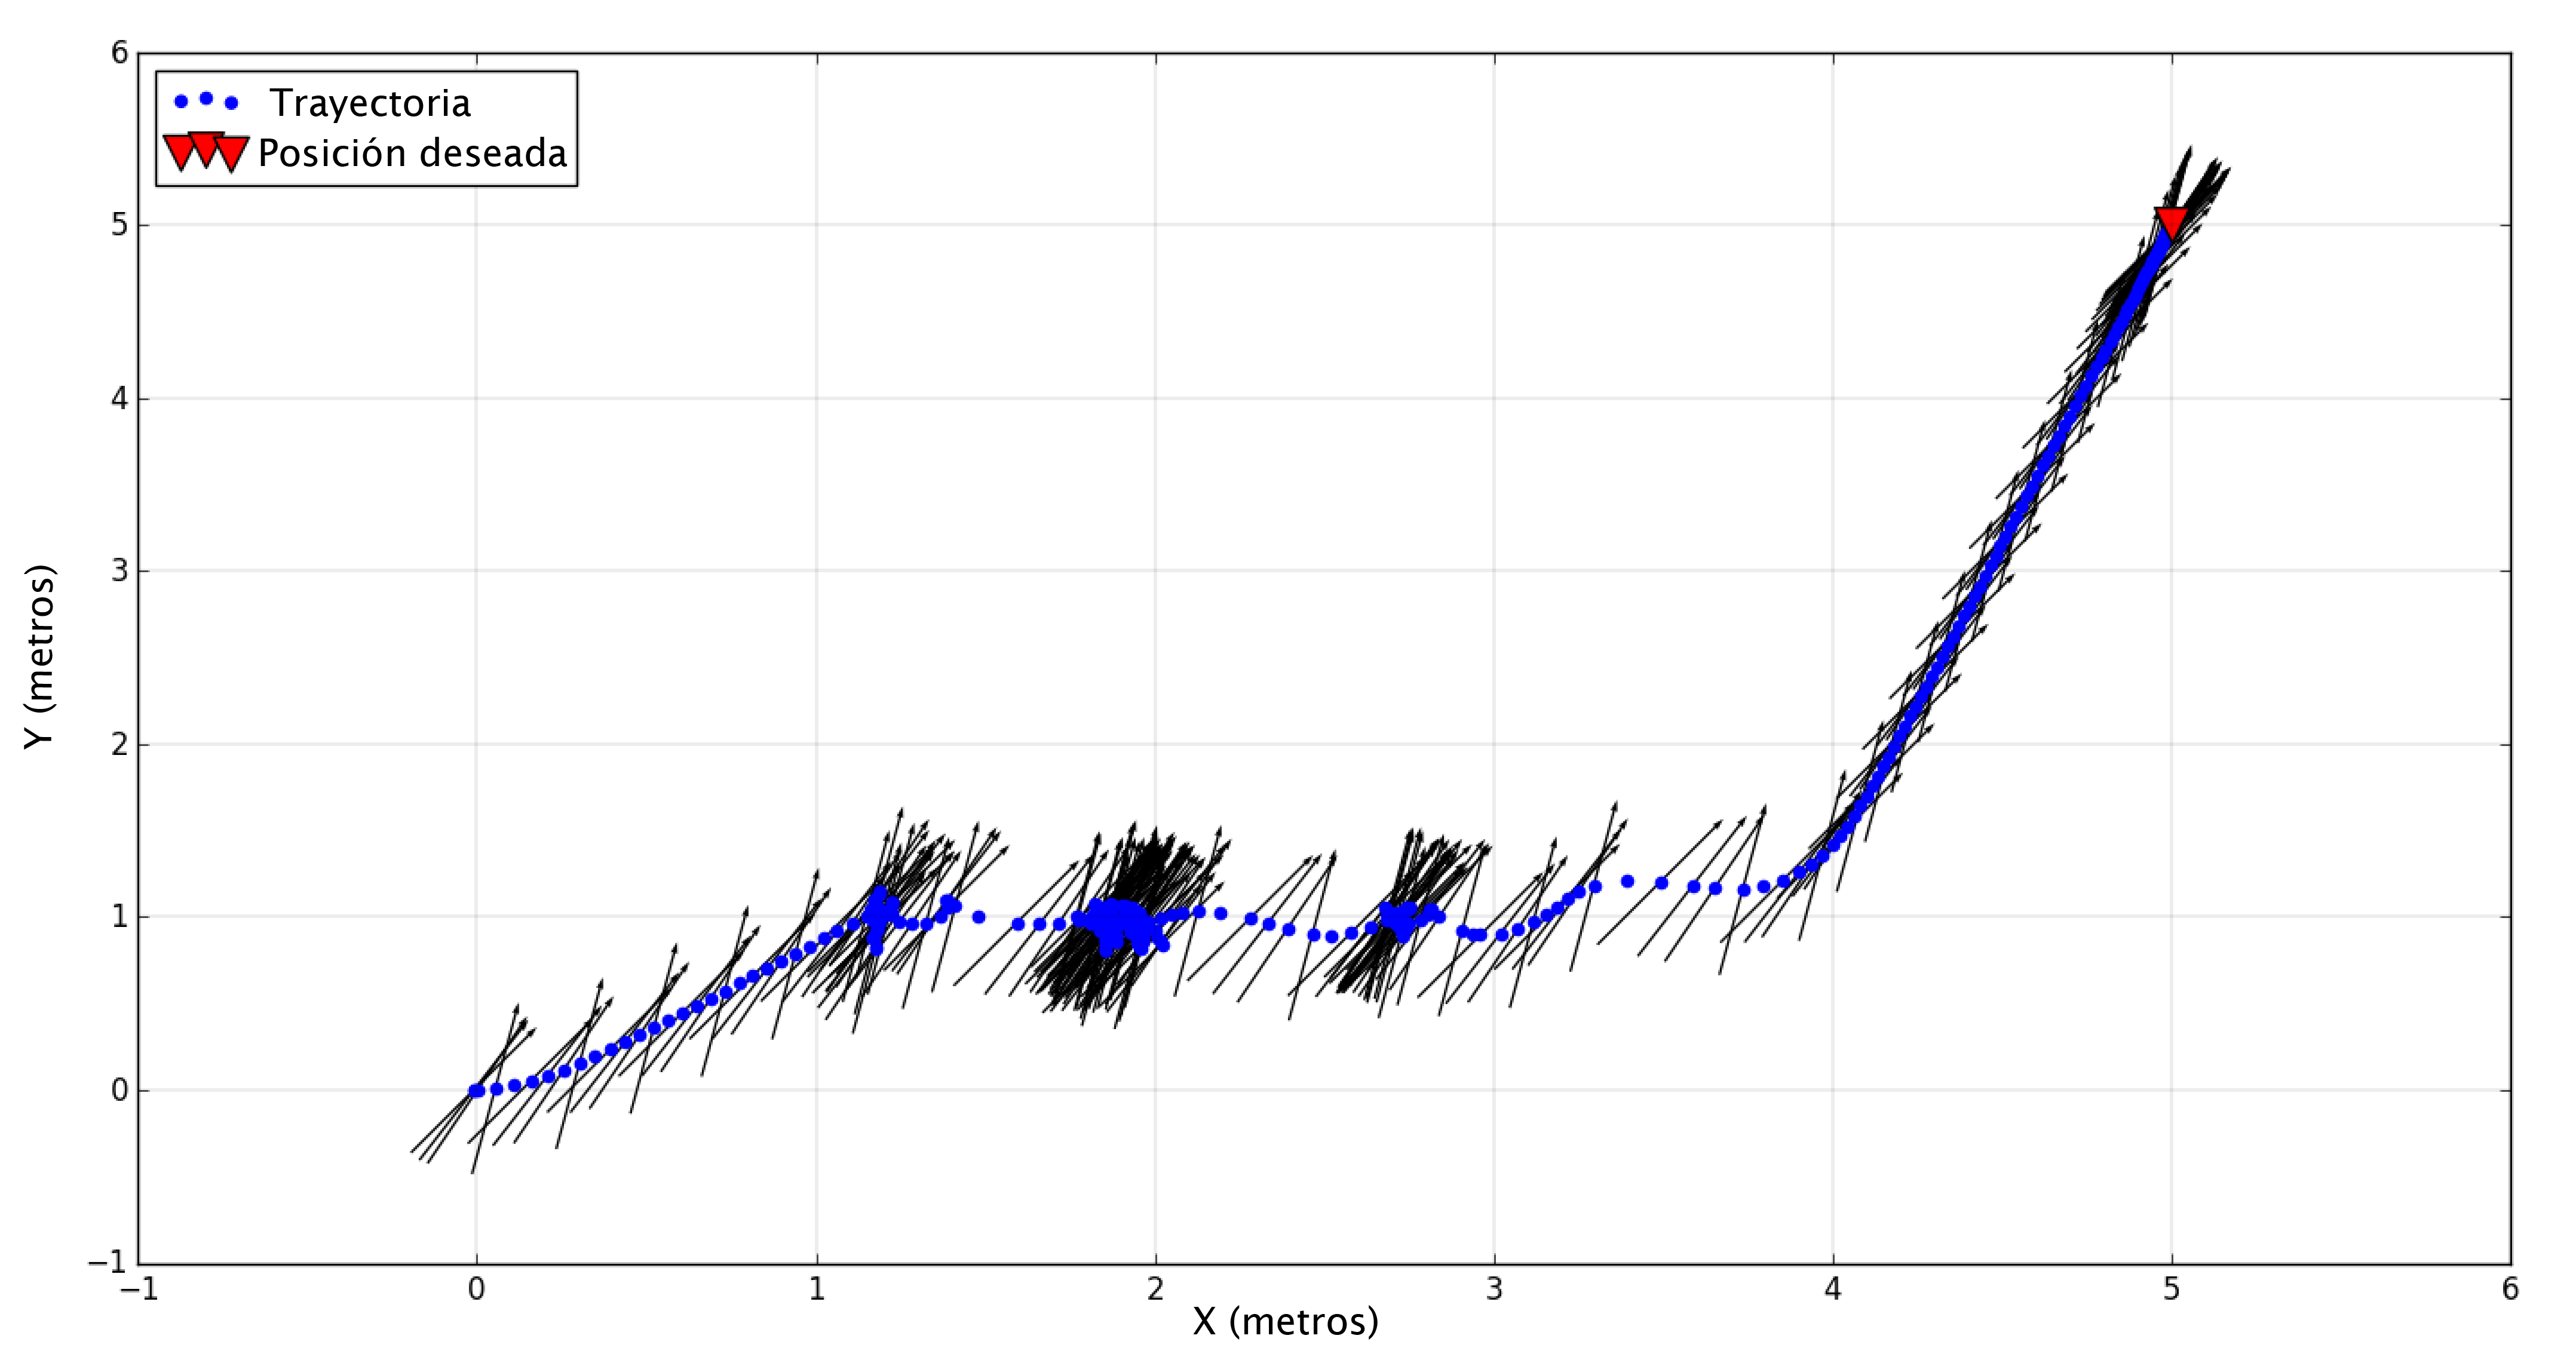
\includegraphics[width=0.80\textwidth]{images/fattr_slam.png}
%  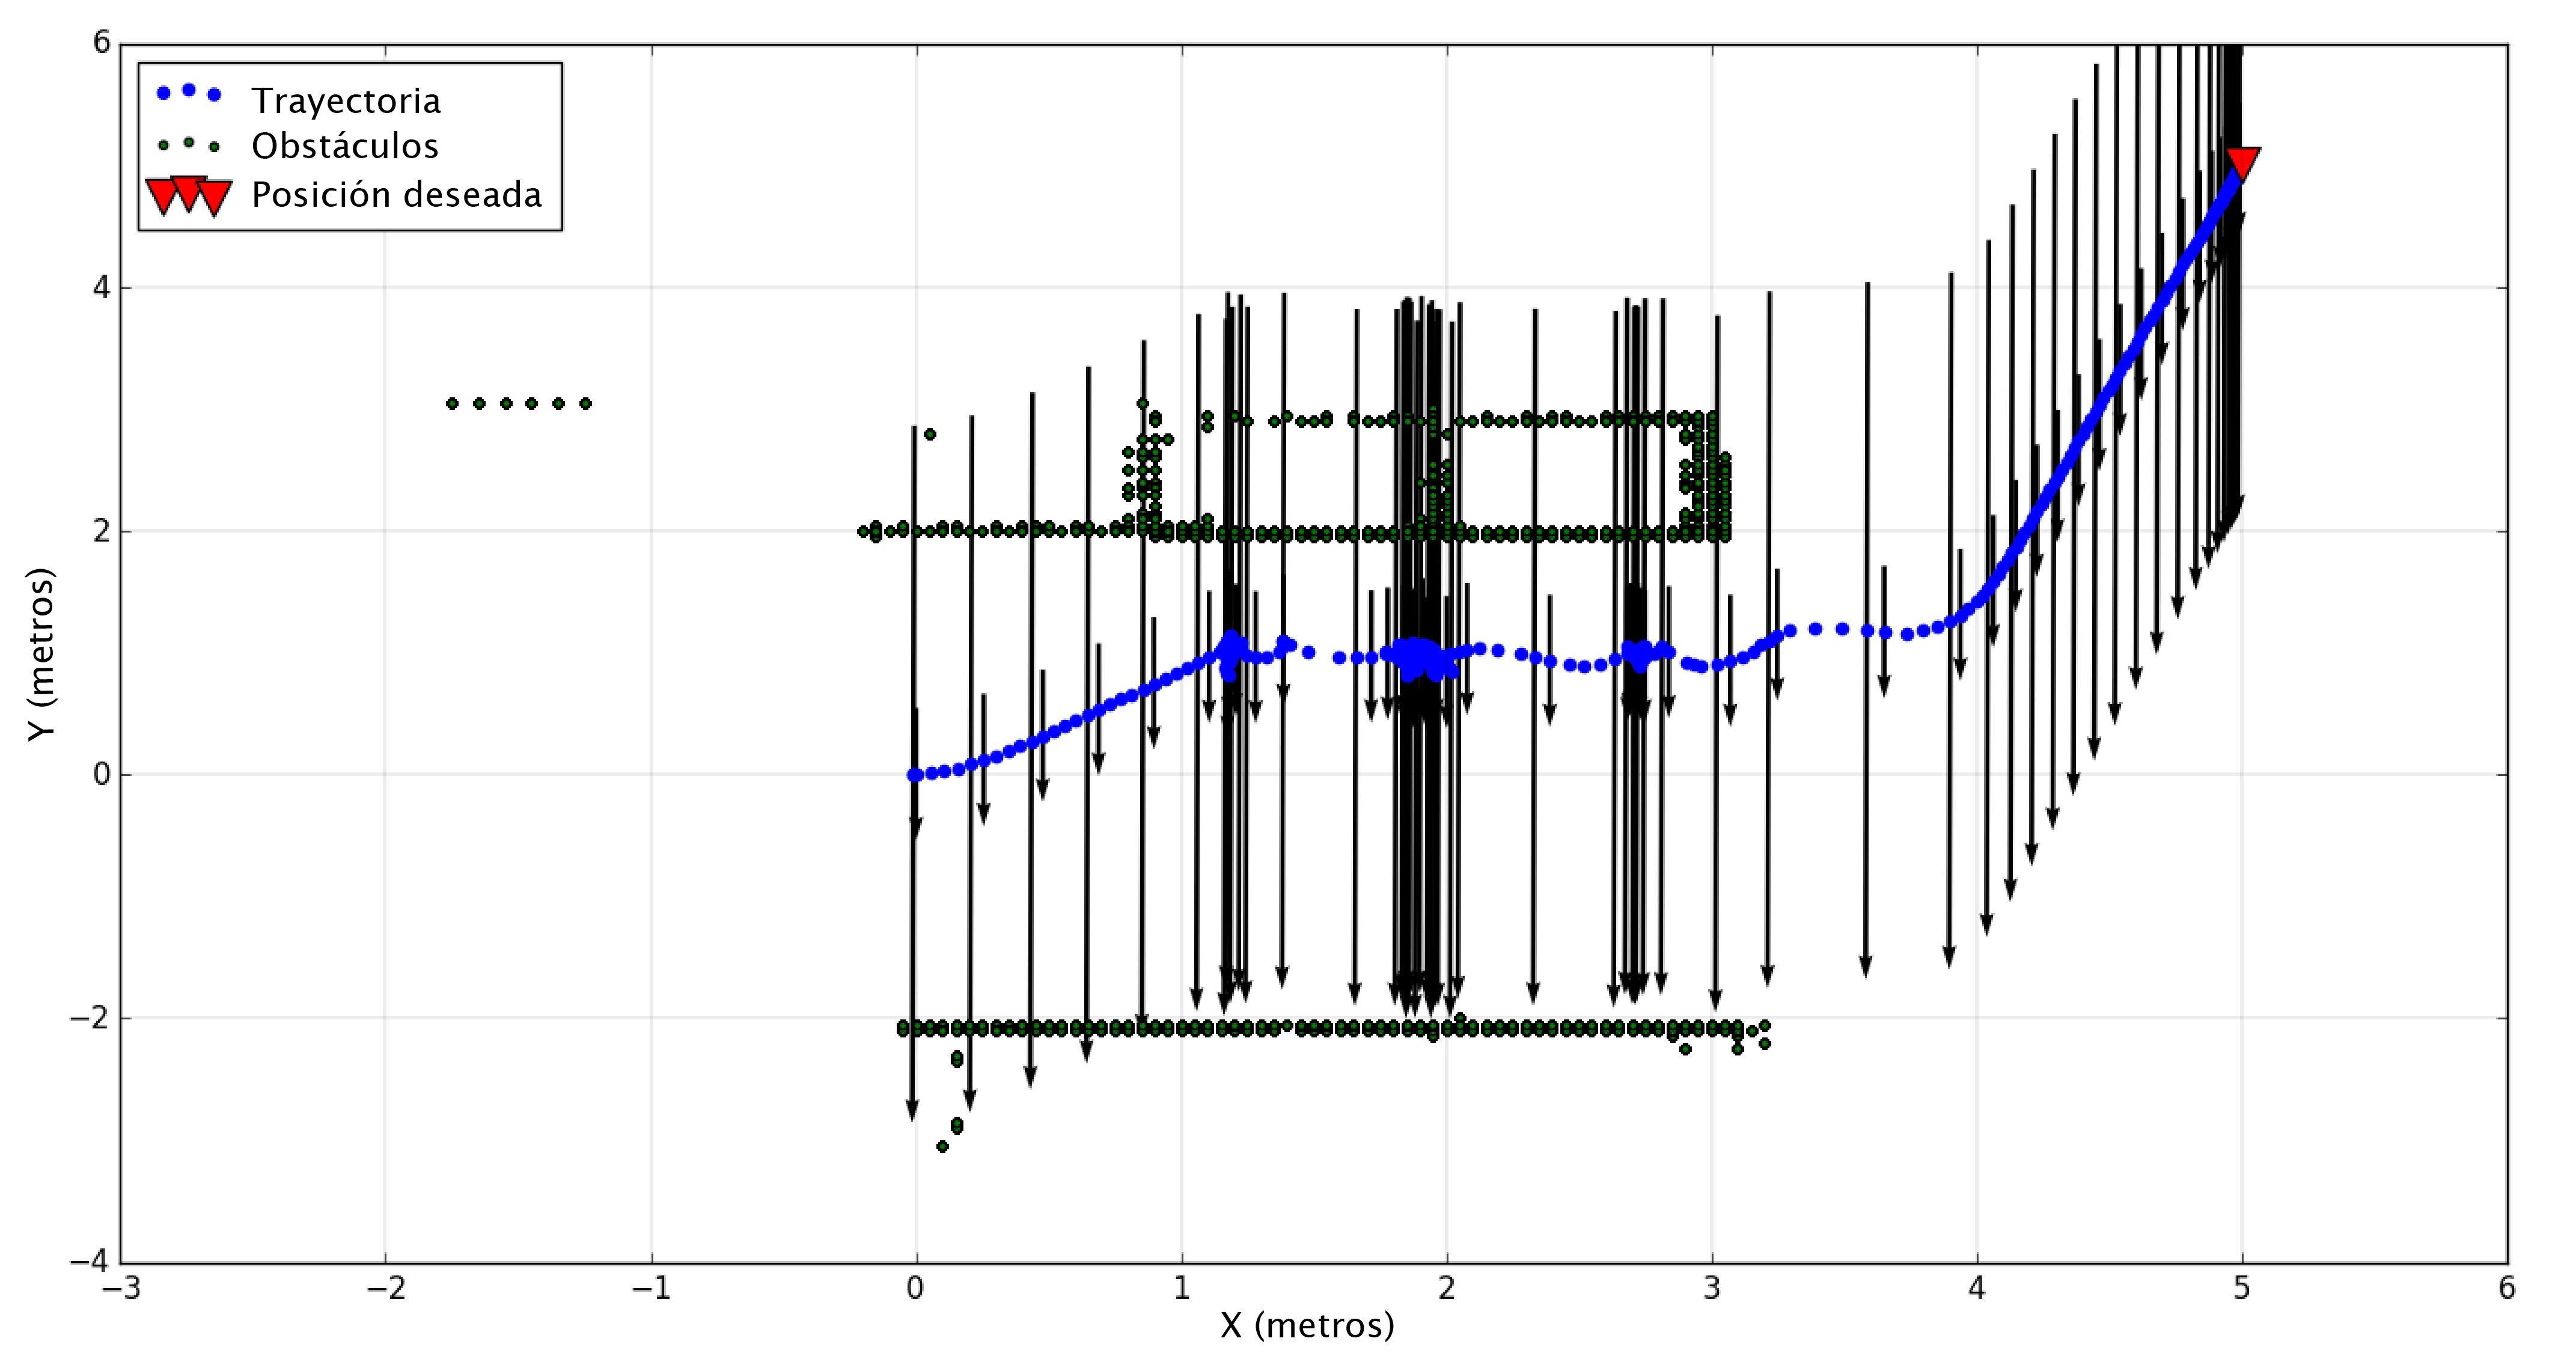
\includegraphics[width=0.80\textwidth]{images/frep_slam.png}
%  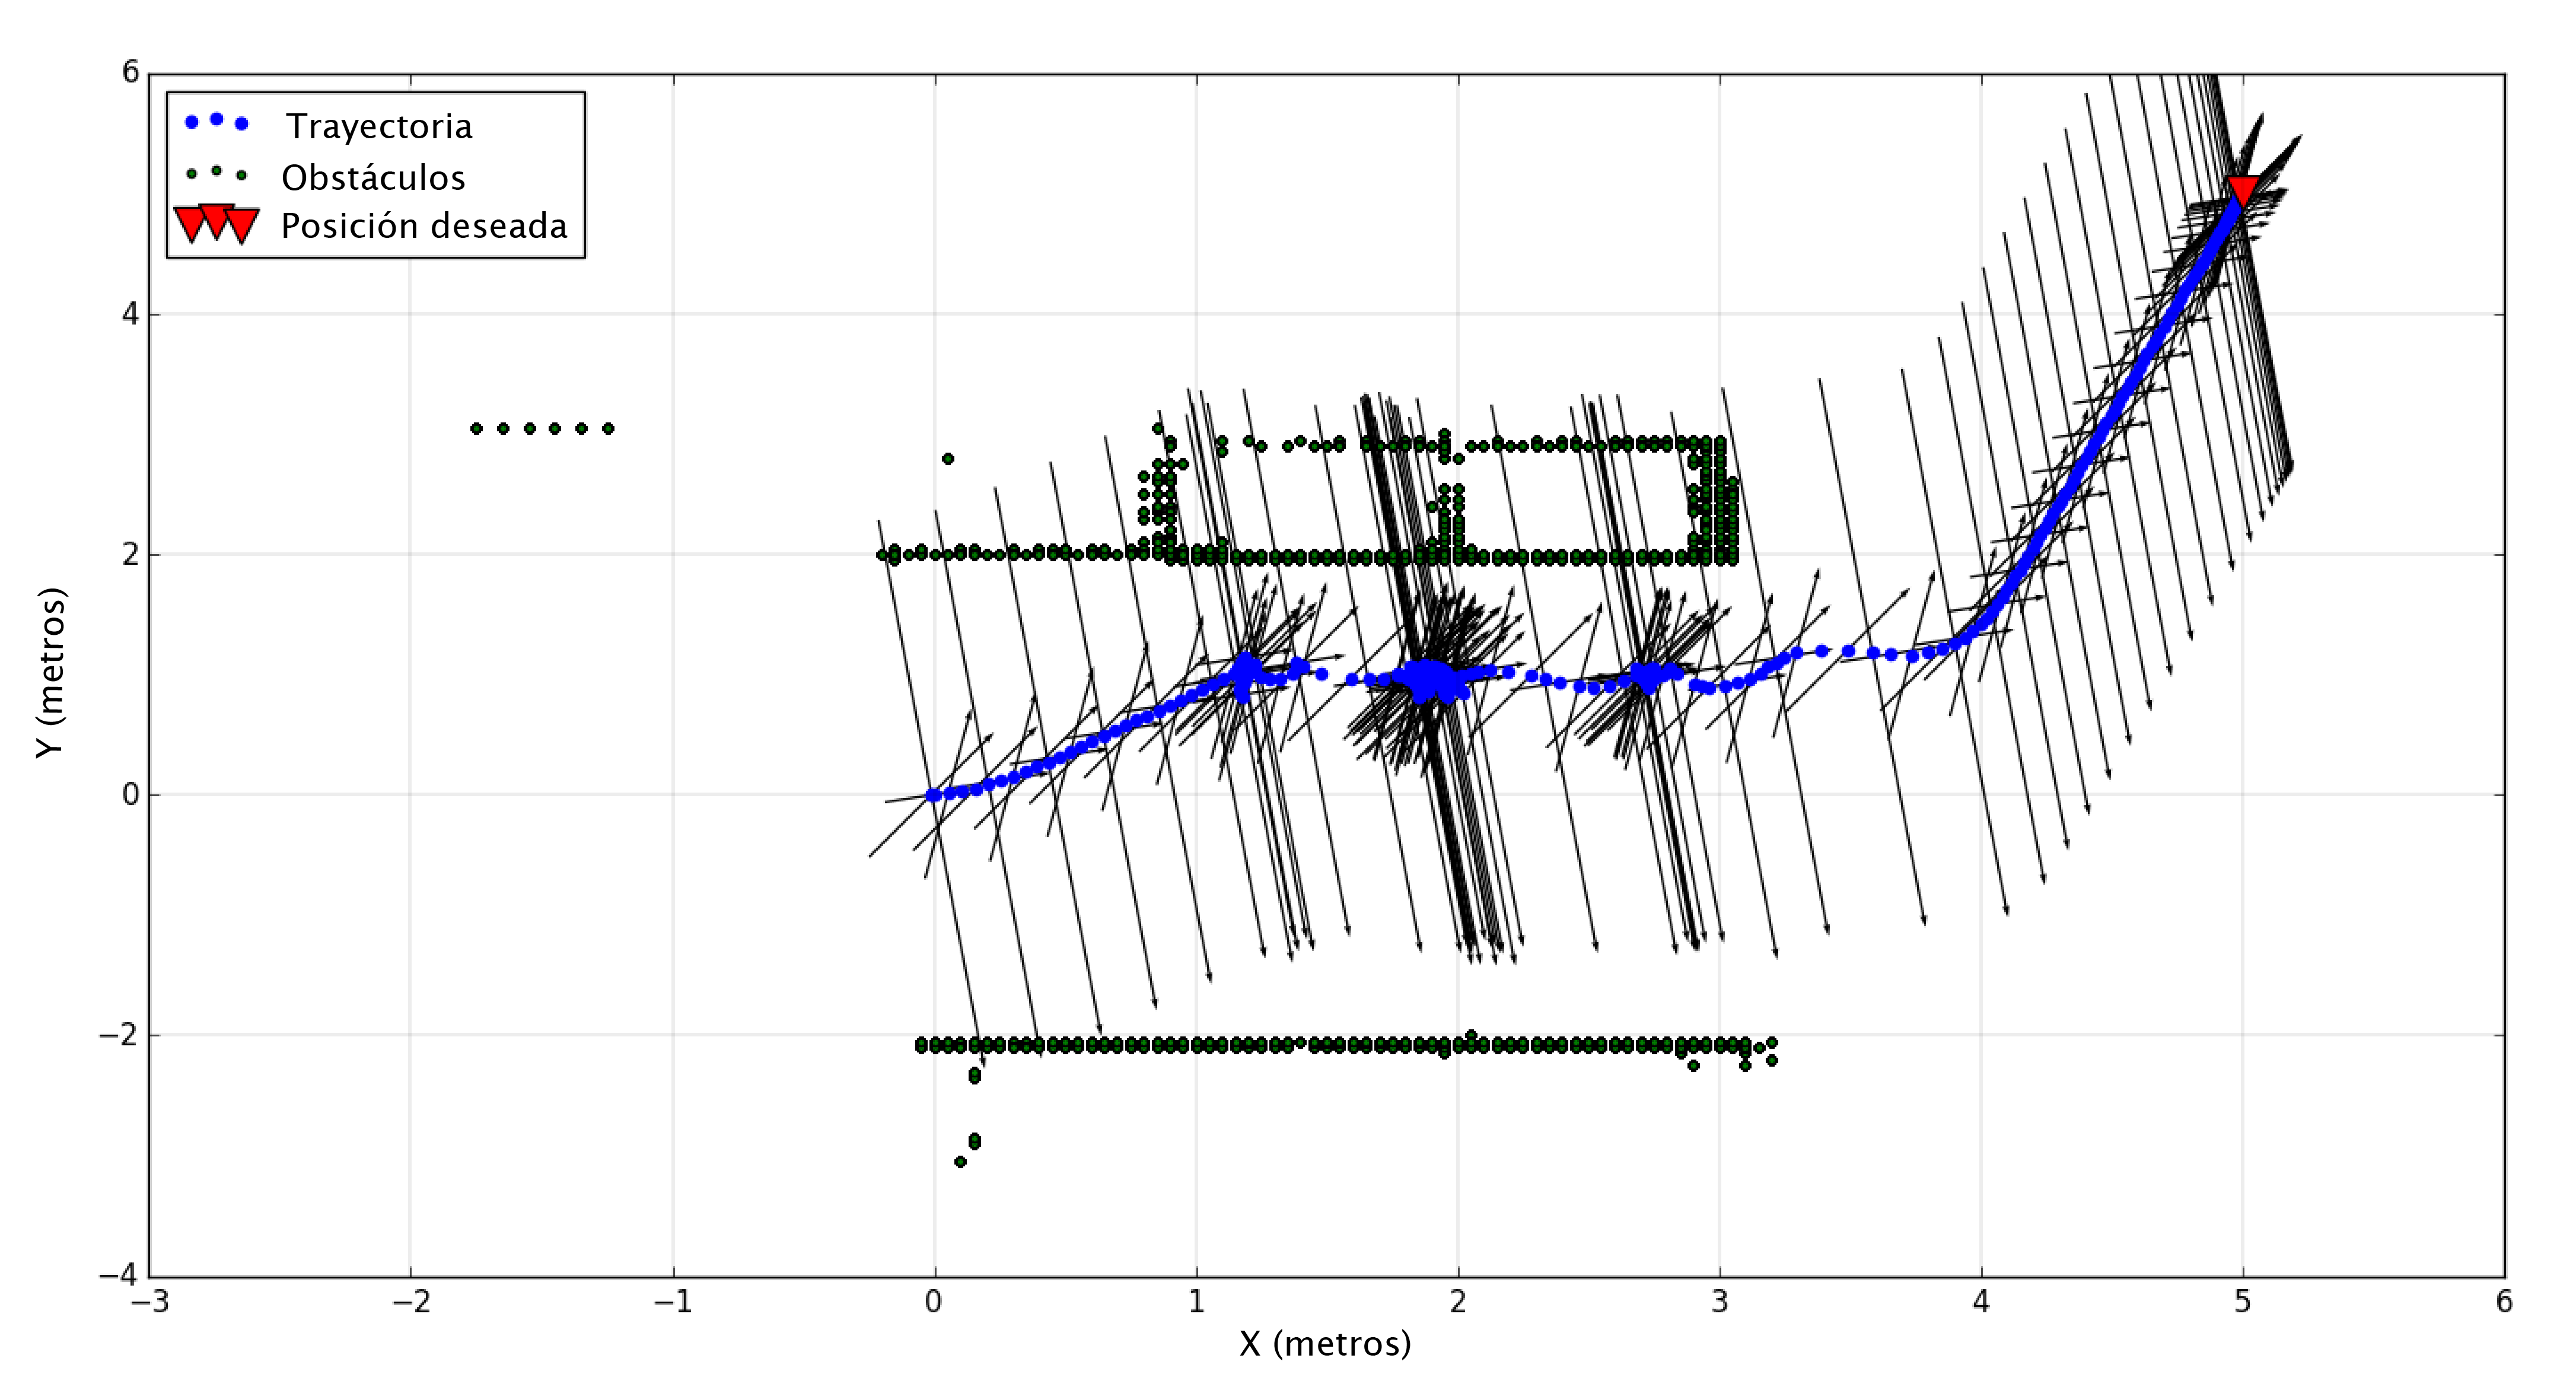
\includegraphics[width=0.80\textwidth]{images/fnav_slam.png}
%  \captionsetup{font=footnotesize}
%  \caption{Campos atractivos y repulsivos, y la trayectoria que el robot real sigue 
%  usando datos en línea provenientes del sensor lidar montado en la parte superior del 
%  Kobuki.}
%  \label{fig:Kbki_slam}
%\end{figure}

Como se mencionó en la sección \ref{sec:GMAPPING}, para realizar esta prueba se utilizó
el paquete de SLAM llamado \textit{gmapping}, dado por ROS. Este paquete permite crear 
un mapa en dos dimensiones a partir de los datos del sensor lídar y la odometría del 
robot móvil. Cuando se ejecuta el paquete de SLAM empieza a crear tópicos por donde se
envían los datos de la odometría del robot y los datos del lídar. Con la información 
recibida por el nodo del \textit{gmapping}, éste publica las dimensiones del entorno, dentro
de un tópico, hacia el robot Kobuki. Para que el robot móvil se pueda desplazar con respecto
a las dimensiones del mapa recibido por el SLAM, su marco de referencia debe ser remplazado
por el marco de referencia del sensor lídar. La precisión del mapa originado por el SLAM es 
buena, debido a que el algoritmo reduce la cantidad de mediciones que envía el sensor lídar
haciendo que el mapa sea uniforme y los obstáculos se encuentren en la posición correcta
dentro del mapa.

%Al momento de iniciar el paquete \textit{gmapping}, 
%este crea tópicos a los cuales se debe enviar los datos de la odometría del robot y los datos 
%del sensor lidar. Con la información dada el nodo de SLAM publica las dimensiones del mapa 
%dentro de un tópico. Para que el Kobuki se mueva con respecto al mapa generado, el marco de 
%referencia del Kobuki se toma como el marco de referencia del sensor lidar. El nodo de 
%SLAM tiene un alcance máximo de mapeo de 8 metros, tiene un tamaño de mapa en píxeles de 
%512 x 512 y una resolución de mapa de 2.5 centímetros por cada celda del mapa. Además el 
%algoritmo muestrea la cantidad de mediciones que envía el lidar, por tal motivo el mapa 
%obtenido es bastante uniforme y preciso con respecto a las posiciones de los obstáculos 
%dentro del mapa. 
Para el desplazamiento autónomo del robot, dentro del escenario creado, se utilizó las 
etapas de localización y mapeo (SLAM), campo potencial más controlador polar que fueron 
explicados en la sección \ref{sec:NavegacionAutonoma}. Como primer paso el sensor lídar 
permite localizar las posiciones de todos los obstáculos dentro del ambiente. Estas 
posiciones son enviadas al algoritmo de campos potenciales para así generar la 
trayectoria. Para realizar esta prueba se elige como posición deseada el punto 
$(x = 5, y = 5)$. En la Figura \ref{fig:Kbki_slam}a se puede denotar los puntos de color 
azul que representan a la trayectoria por el cual el robot Kobuki se ha desplazado. La 
trayectoria va desde la posición $(x = 0, y = 0)$ donde comenzó el robot hasta la posición
deseada que está representada por un triángulo invertido de color rojo. También se puede 
ver que hay flechas de color negro que tienen diferentes tamaños y diferentes direcciones.
El tamaño de la flecha indica la velocidad lineal a la que el robot debe desplazarse y 
la dirección indica la orientación necesaria para que el robot pueda llegar a la 
posición deseada.

%Para  realizar que el robot se pueda desplazar de forma autónoma dentro del ambiente,se 
%obtiene las posiciones del mapa ($X_{M}, Y_{M}$), los cuales son enviados al algoritmo 
%de campos potenciales como obstáculos para que el robot pueda generar su propia 
%trayectoria. Para realizar esta prueba se elige una posición deseado en el mapa. La 
%posición deseada es $(x = 5, y = 5)$. En la Figura \ref{fig:Kbki_slam}a se muestra 
%la trayectoria del robot (puntos azules) que se va desplazando hacia la posición 
%deseada. Además se puede ver que las flechas de color negro tienen una dirección, esto
%indica la orientación necesaria que debe tener el robot para que llegue hacia la meta, 
%asimismo el tamaño de las flechas indican la velocidad a la que debe ir el robot para 
%que llegue al punto deseado. 

En la Figura \ref{fig:Kbki_slam}b los puntos verdes representan a los obstáculos dentro
del escenario, como se puede observar los puntos son uniformes y alineados. El algoritmo
SLAM del paquete de \textit{gmapping} se encarga de reducir la cantidad de mediciones del
sensor lídar, luego añade los datos de la odometría haciendo que la estimación de las 
posiciones de los objetos dentro del ambiente sea de forma clara y precisa. En esta figura
también se puede observar las flechas del campo de repulsión, donde cada flecha tiene una
dirección hacia afuera en cada obstáculo. El tamaño de las flechas va acorde con la 
trayectoria del robot Kobuki, esto quiere decir que mientras el robot se encuentre más
cerca al obstáculo el tamaño de la flecha será más grande y por ende la fuerza de 
repulsión será mayor. Estas fuerzas ayudan a que el robot pueda evadir los obstáculos
y evitar las colisiones. 

Finalmente, en la Figura \ref{fig:Kbki_slam}c se muestra las sumas de fuerzas de atracción y
repulsión. La suma de estas fuerzas generan la trayectoria que debe realizar el robot
para llegar a la posición deseada, evitando los obstáculos. En esta figura se puede observar
que en algunas regiones de la trayectoria se nota una concentración de fuerzas de navegación. Esto se debe a la interacción de su movimiento autónomo, ya que el robot va retrocediendo para
evitar el choque originado por el campo de repulsión y a su vez se encuentra atraído hacia 
la posición deseada originado por el campo de atracción.

%En la Figura \ref{fig:Kbki_slam}b se muestra los obstáculos (puntos verdes), se 
%aprecia con mayor claridad y uniformidad las posiciones de los obstáculos. Esto se debe 
%a que el algoritmo muestrea la cantidad de mediciones que hace el sensor lidar y añade 
%la odometría del robot, permitiendo estimar con mayor precisión las posiciones de los 
%obstáculos. También se puede observar las flechas de color negro que tienen una dirección 
%hacia afuera de los obstaćulos. La dirección de las flechas es según la trayectoria 
%(puntos azules) del robot, en este caso el robot se acerca hacia los obstáculos que se 
%encuentran en los valores del eje $Y$ positivo y el algoritmo de campos potenciales 
%genera fuerzas de repulsión para que el robot evite los obstáculos. Se muestra una 
%acumulación de puntos en diferentes partes de la trayectoria, y a su vez se nota una 
%mayor concentración de fuerzas de repulsión en dichas partes, esto se debe a la interacción 
%del movimiento del robot para no chocarse con los obstáculos y generar una nueva trayectoria 
%hacia el punto deseado. Finalmente, en la Figura \ref{fig:Kbki_slam}c se muestra las sumas 
%de las fuerzas de atracción y las fuerzas de repulsión que hacen que el robot pueda ir a la 
%posición deseada y a su vez evite los obstáculos del lugar.

\begin{figure}
  \centering \footnotesize
  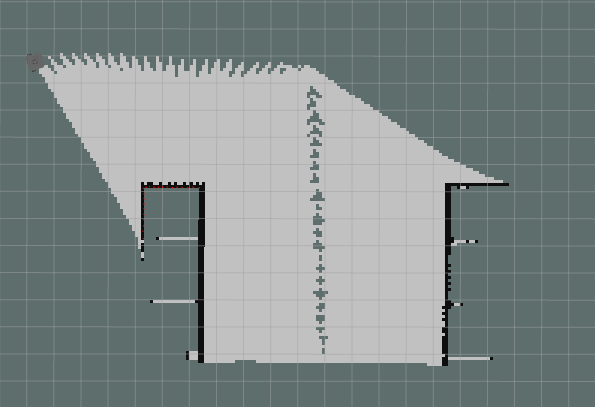
\includegraphics[width=0.80\textwidth]{images/map_slam.png}
  \captionsetup{font=footnotesize}
  \caption{Mapa en dos dimensiones obtenido del algoritmo SLAM, el mapa es 
  visualizado en la herramienta Rviz.}
  \label{fig:SLAM_2D}
\end{figure}

La Figura \ref{fig:SLAM_2D} muestra el mapa generado por el paquete \textit{gmapping}. Como 
se puede ver en la imagen, el mapa está compuesto por tres colores diferentes. Estos
colores fueron descritos en la sección \ref{sec:GMAPPING}. Este mapa ayuda al robot
a tener una información precisa del lugar donde se encuentra navegando. El robot pudo
generar su propia trayectoria con la información brindada por el algoritmo SLAM haciendo
que pueda llegar a la posición deseada mientras evitaba los obstáculos en su camino.

%Cada color de la imagen tiene un significado. El color verdoso significa un lugar 
%desconocido, esto quiere decir los lugares por donde el robot móvil no ha explorado o 
%navegado. El color plomo claro, significa un lugar conocido, esto quiere decir el lugar por 
%donde el robot móvil o el sensor lidar ha recorrido. Finalmente, el color negro este color 
%representa a los obstáculos mapeado dentro del entorno explorado. Este mapa ayuda a que el 
%robot pueda reconocer con exactitud los lugares que ha explorado, los obstáculos y los lugares 
%que aún le falta por recorrer.

\section{Resultados del mapeo en tres dimensiones con el sistema mecánico}

En esta sección se muestra las pruebas que fueron realizadas para la construcción
tridimensional de un ambiente real. Se utilizó el sistema mecánico que fue construido 
(ver Figura \ref{f:lidar3D}c) y explicado en la sección \ref{sec:SistP3D}. Las pruebas 
realizadas fueron unicamente con el sistema mecánico de forma estática y no montado al robot 
diferencial. Estas pruebas sirvieron para validar el algoritmo de construcción 
en tres dimensiones.

%En esta sección se explicará las pruebas que se realizaron para poder validar el mapa en 
%tres dimensiones con el sistema mecánico propuesto. Se realizarón pruebas de validación 
%del algoritmo para la construcción del mapa en 3D dentro de una caja cerrada y dentro de 
%un pasadizo cerrado. Las pruebas consistieron en dejar el sistema mecánico de manera 
%estática y empezar a realizar mediciones mientras el lidar giraba en 360\grad~ y el 
%servomotor rotaba en un ángulo de abertura de $\pm$ 15\grad~.

\subsection{Construcción tridimensional de una caja}
\label{sec:MapaCaja}
\begin{figure}
  \centering \footnotesize
  %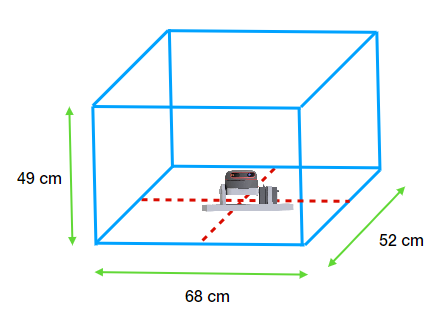
\includegraphics[width=0.70\textwidth]{images/caja_lidar3D.png}
  %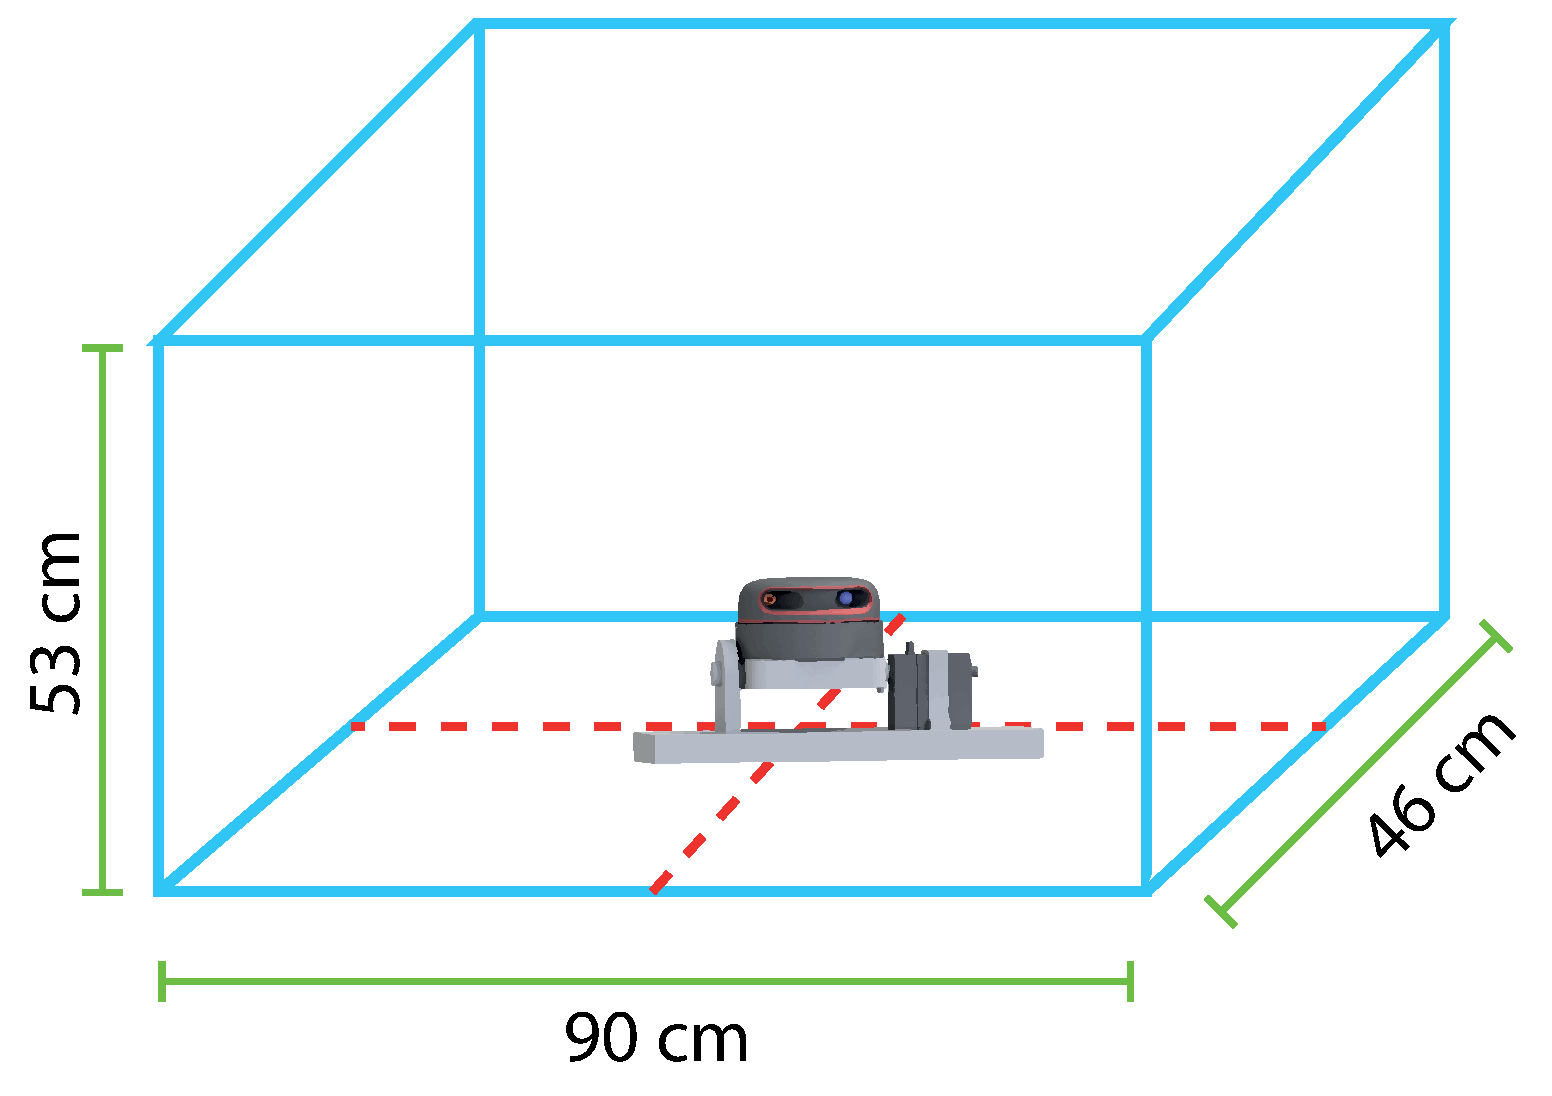
\includegraphics[width=0.70\textwidth]{images/cajalidar3d.eps}
  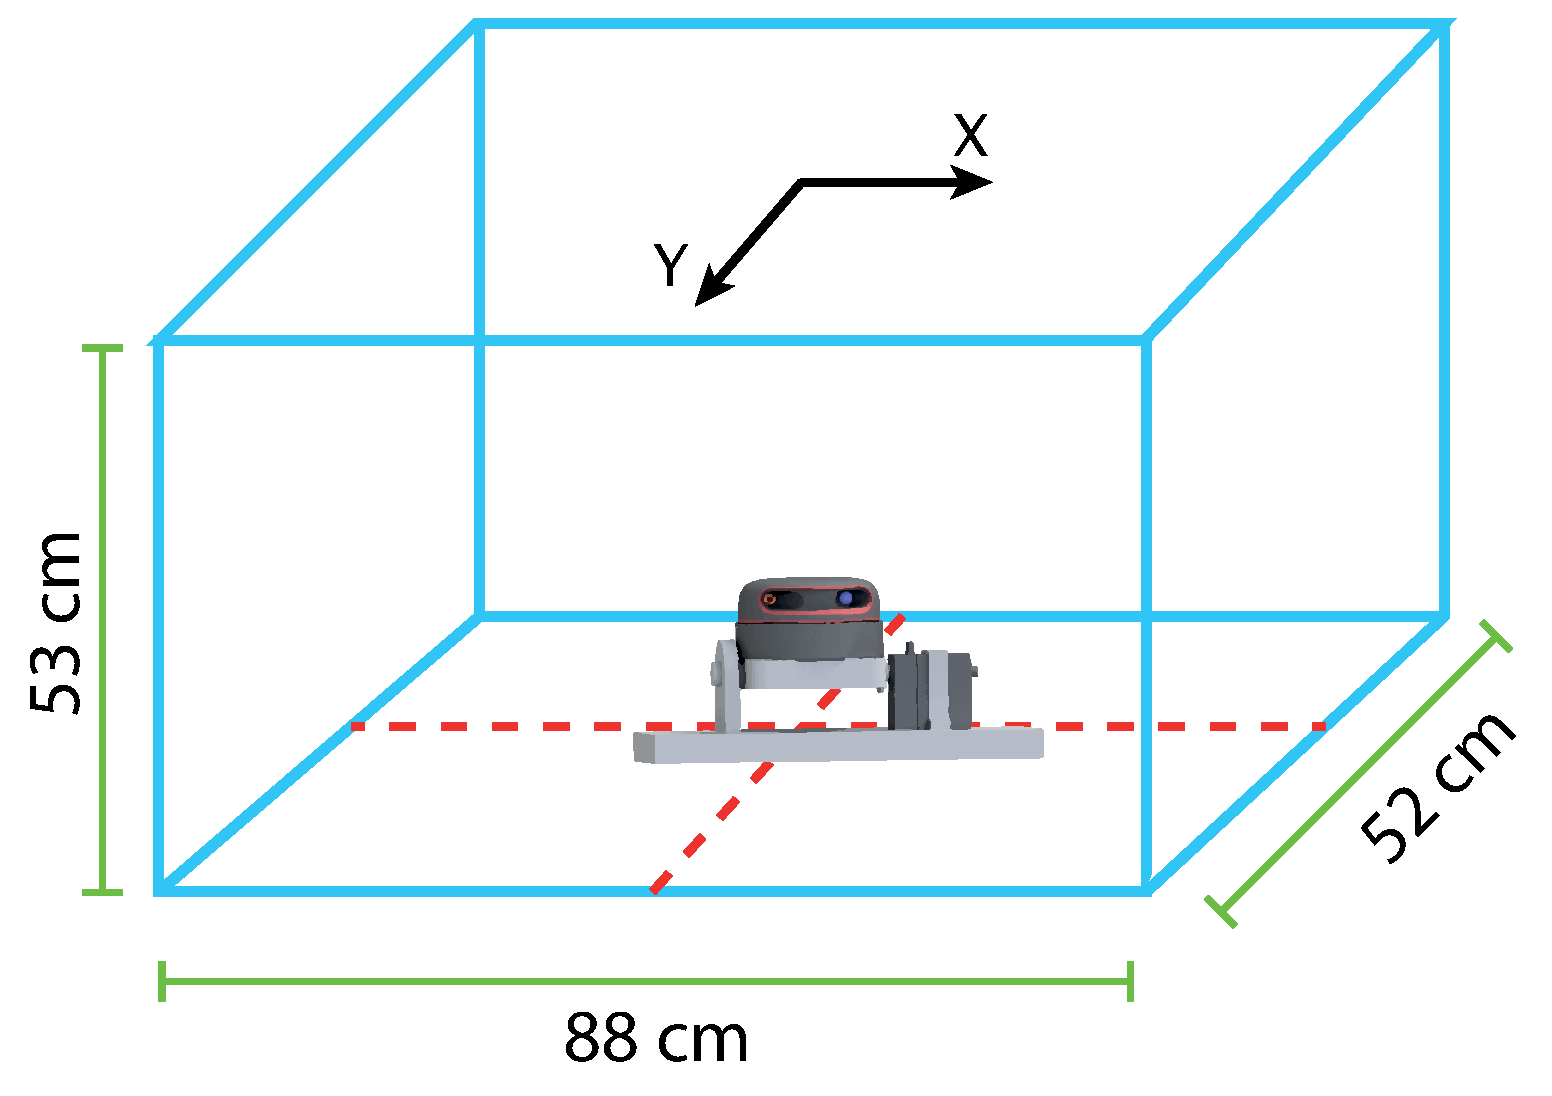
\includegraphics[width=0.70\textwidth]{images/3DLidar.eps}
  \captionsetup{font=footnotesize}
  \caption{Dimensiones de la caja donde se realizó las mediciones de forma interna, para
  generar la construcción en tres dimensiones.}
  \label{fig:dim_cajaReal}
\end{figure}

En esta prueba se utilizó una caja real con las dimensiones mostradas en 
la Figura \ref{fig:dim_cajaReal}. Para poder realizar esta prueba se tuvo que
colocar el sistema mecánico dentro de la caja, haciendo que el sensor lídar 
se posicione en el centro de la caja como se muestra en la Figura 
\ref{fig:dim_cajaReal}. Además en esta figura se muestra un sistema de referencia por 
encima del sensor lídar, el cual hace referencia a la posición ($x = 0, y = 0$) 
de la caja. Este sistema de referencia ayuda a conocer las posiciones de las paredes de 
la caja. Una vez colocado el sistema mecánico dentro de la caja, se 
tomó mediciones durante 40 segundos. El sistema mecánico es controlado por
medio de un Raspberry Pi3, donde el microcontrolador recibe la información 
de los componentes del sistema mecánico y envía estos datos hacia una computadora
de forma remota. Los datos recibidos son almacenados para el procesamiento posterior.

%Para realizar la primera prueba, se utilizó una caja real en el cual fue colocado 
%el sistema mecánico del sensor lidar para realizar las mediciones. En la Figura 
%\ref{fig:dim_cajaReal} se muestra las dimensiones de la caja donde se hizo las 
%pruebas. Como primer paso se coloco el sistema mecánico en el centro de la caja, esto
%ayuda a conocer las posiciones de las paredes de la caja en el plano cartesiano. Una 
%vez colocado el sensor, fue dejado por 40 segundos para que realicé las mediciones del 
%ambiente. El sensor lidar y el servomotor fueron controlados a través de un Raspberry 
%Pi3. La información enviada por el sensor y el servomotor son recibidos por el Raspberry 
%Pi3, el cual se encarga de enviar los datos de forma remota hacia una computadora. Estos 
%datos son almacenados para ser procesadas posteriormente.

\begin{figure}[ht!]
     %\begin{center}
     \centering
     \begin{tabular}{cc}
        %\subfigure[]{\label{fig:etiquetaA}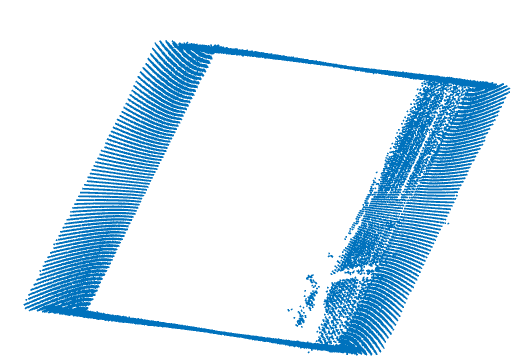
\includegraphics[width=.32\textwidth]{images/caja3D_1.png}}
        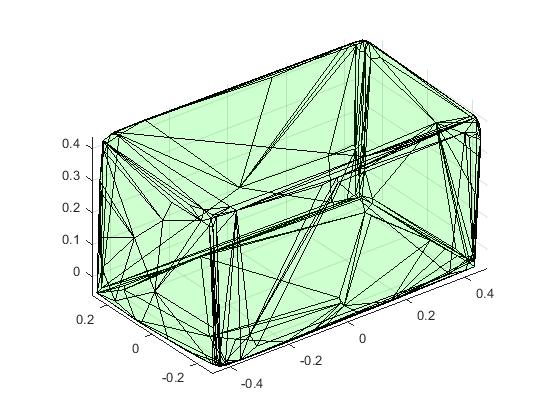
\includegraphics[width=.50\textwidth]{images/1.jpg}&
        %\subfigure[]{\label{fig:etiquetaB}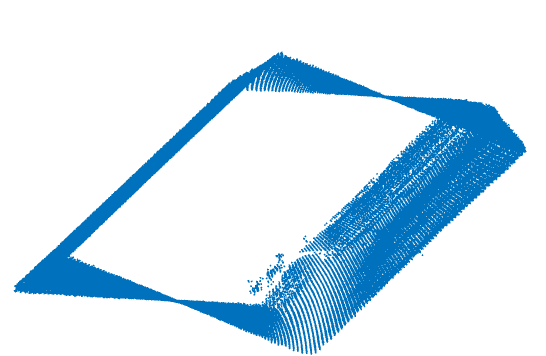
\includegraphics[width=.32\textwidth]{images/caja3D_2.png}}
        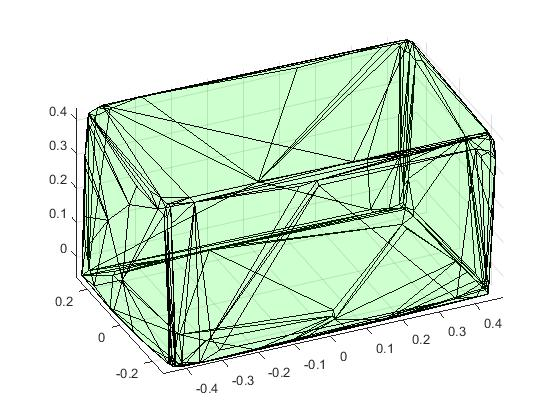
\includegraphics[width=.50\textwidth]{images/2.jpg}\\
        (a)&(b)\\
        %\subfigure[]{\label{fig:etiquetaC}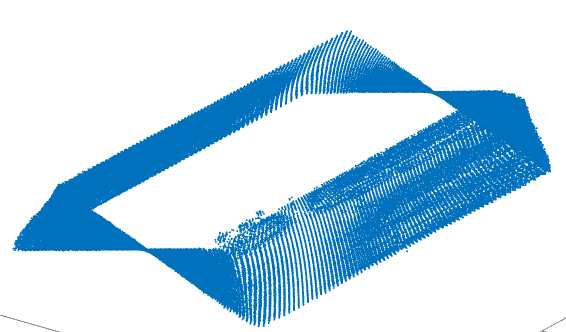
\includegraphics[width=.32\textwidth]{images/caja3D_3.png}}
        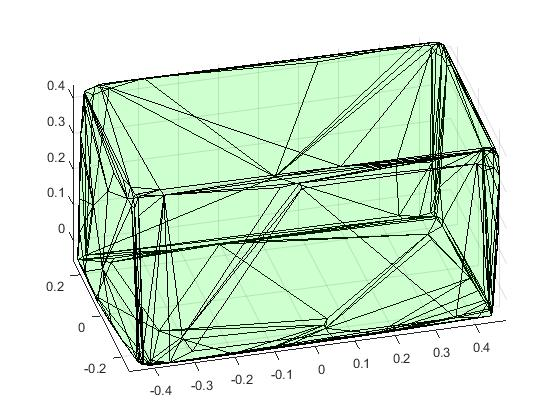
\includegraphics[width=.50\textwidth]{images/3.jpg}&
        %(a)&(b)&(c)\\
        %\subfigure[]{\label{fig:etiquetaC}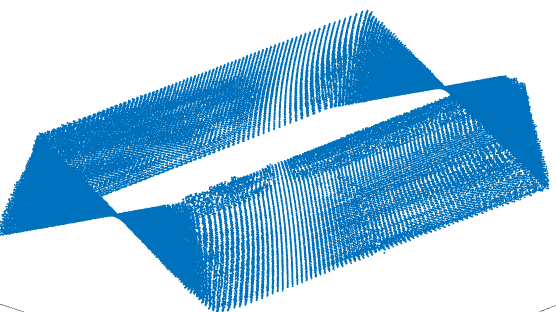
\includegraphics[width=.32\textwidth]{images/caja3D_4.png}}
        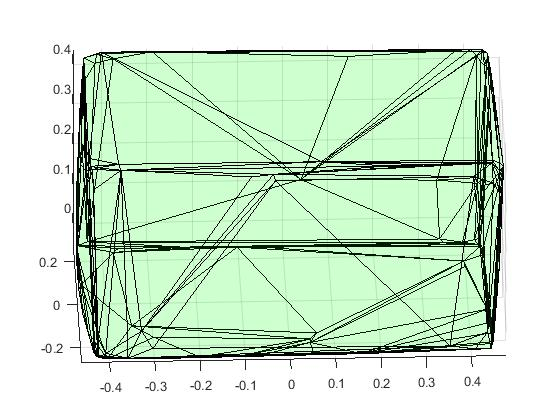
\includegraphics[width=.50\textwidth]{images/4.jpg}\\
        (c)&(d)\\
        %\subfigure[]{\label{fig:etiquetaC}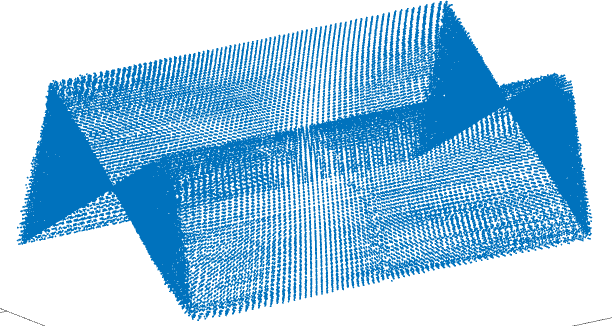
\includegraphics[width=.32\textwidth]{images/caja3D_5.png}}
        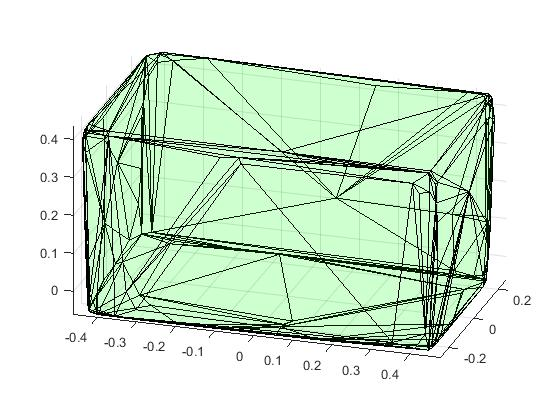
\includegraphics[width=.50\textwidth]{images/5.jpg}&
        %\subfigure[]{\label{fig:etiquetaC}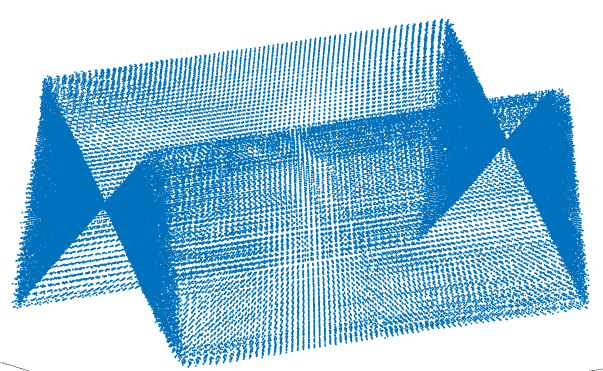
\includegraphics[width=.32\textwidth]{images/caja3D_6.png}}
        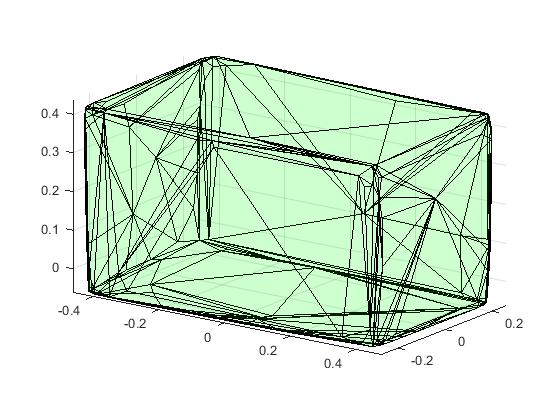
\includegraphics[width=.50\textwidth]{images/6.jpg}\\
        (e)&(f)
        %(d)&(e)&(f)\\
        %\subfigure[]{\label{fig:etiquetaC}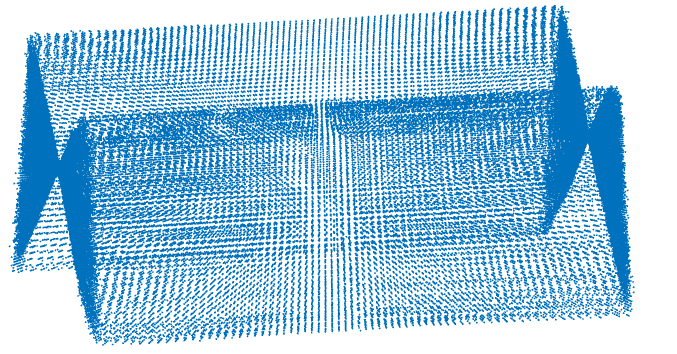
\includegraphics[width=.32\textwidth]{images/caja3D_7.png}}
       % 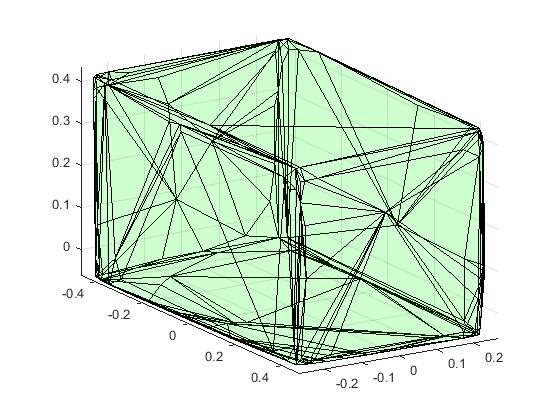
\includegraphics[width=.33\textwidth]{images/7.jpg}&
        %\subfigure[]{\label{fig:etiquetaC}\includegraphics[width=.32\textwidth]{images/caja3D_8.png}}
       % \includegraphics[width=.33\textwidth]{images/8.jpg}&
        %\subfigure[]{\label{fig:etiquetaC}\includegraphics[width=.32\textwidth]{images/caja3D_9.png}}
       % \includegraphics[width=.33\textwidth]{images/9.jpg}\\
        %(g)&(h)&(i)
       % \includegraphics[width=.33\textwidth]{images/10.jpg}&
       % \includegraphics[width=.33\textwidth]{images/11.jpg}&
       % \includegraphics[width=.33\textwidth]{images/12.jpg}\\
    %\end{center}
    \end{tabular}
  \captionsetup{font=footnotesize}
    \caption{\label{fig:Caja3D}Construcción del sólido geométrico, a partir de 
    las mediciones del sensor lídar. El crecimiento del sólido tridimensional 
    rota en sentido horario.}
\end{figure}

%\begin{figure}
%  \centering \footnotesize
%  \includegraphics[width=0.40\textwidth]{images/caja3D_1.png}
%  \includegraphics[width=0.40\textwidth]{images/caja3D_2.png}
%  \includegraphics[width=0.40\textwidth]{images/caja3D_3.png}
%  \includegraphics[width=0.40\textwidth]{images/caja3D_4.png}
%  \includegraphics[width=0.40\textwidth]{images/caja3D_5.png}
%  \includegraphics[width=0.40\textwidth]{images/caja3D_6.png}
%  \includegraphics[width=0.40\textwidth]{images/caja3D_7.png}
%  \includegraphics[width=0.40\textwidth]{images/caja3D_8.png}
%  \includegraphics[width=0.50\textwidth]{images/caja3D_9.png}
%  \captionsetup{font=footnotesize}
%  \caption{Mapa en tres dimensiones de una caja. El crecimiento del mapa tridimensional 
%  de la caja va en sentido horario.}
%  \label{fig:Caja3D}
%\end{figure}

En la sección \ref{sec:Sistema3D} se explicó de forma detallada los pasos que 
se debe seguir para construir un sólido tridimensional en un ambiente real, 
usando el sensor lídar y el motor paso a paso. Las mediciones realizadas fueron 
dibujadas usando \textit{python}, y se obtuvo
el sólido mostrado en la Figura \ref{fig:Caja3D}, donde la imagen va rotando en 
sentido horario. Esta figura muestra un prisma rectangular, donde las caras del 
sólido se encuentran planas y las líneas de las aristas son continuas. Asimismo, 
se puede observar que existen líneas que se entrelazan entre algunas aristas del 
sólido. Esto se debe al algoritmo que permite gráficar la nube de puntos en un 
sólido geométrico.

El diseño mecánico del sistema, permite al sensor lídar tomar mediciones en cada 
rincon de la caja. Por ende, se puede notar que la caja presenta muy pocas 
imperfecciones. El sólido gráficado, a simple vista, tiene las mismas dimensiones 
de la caja real. Para estimar el error que existe en las posiciones, en el 
plano cartesiano, de la nube de puntos con respecto a la caja se colocó el sistema 
dentro de la caja, haciendo que el sensor lídar se posicione lo más cercano al 
centro de la caja. Con la nueva posición del sensor lídar se puede corroborar si 
la nube de puntos originada se encuentra en la misma posición en la que 
se encuentran cada una de las paredes de la caja.

\begin{figure}%[ht!]
    \centering
    \begin{tabular}{c}
      \includegraphics[width=.70\textwidth]{images/ErrRegionIZQX.eps}\\
      (a)\\
      \includegraphics[width=.70\textwidth]{images/ErrRegionDERX.eps}\\
      (b)
    \end{tabular}
  \captionsetup{font=footnotesize}
    \caption{\label{f:EstadisticaX}Histogramas de la cantidad de muestras con 
    respecto a la posición en el eje $\mayusx$ del sólido geométrico. En (a) se 
    muestra el histograma de la pared izquierda del sólido con una posición de 
    $\mayusx = -0.44~m$ y en (b) se muestra el histograma de la pared derecha con una
    posición de $\mayusx = 0.44~m$. }
\end{figure}

%\begin{figure}
%  \centering \footnotesize
%  \includegraphics[width=0.90\textwidth]{images/hist_izquierda_caja.png}
%  \captionsetup{font=footnotesize}
%  \caption{Distribución normal del lado izquierdo de la caja real.}
%  \label{fig:hist_Izq}
%\end{figure}

%\begin{figure}
%  \centering \footnotesize
%  \includegraphics[width=0.90\textwidth]{images/hist_derecha_caja.png}
%  \captionsetup{font=footnotesize}
%  \caption{Histograma del lado derecho de la caja real.}
%  \label{fig:hist_Dere}
%\end{figure}

Para poder diferenciar cada pared de la caja se toma como referencia la posición 
del sensor lídar. Cuando el sensor lídar comienza a funcionar, la posición donde
se encuentre es considerada como ($x = 0~m, y = 0~m$). Como el sensor
se encuentra en el centro de la caja, las posiciones de cada pared serán las 
siguientes: en el eje $\mayusx$ las posiciones de cada pared son $\mayusx = -0.44~m$ 
y $\mayusx = 0.44~m$; en el eje $\mayusy$ las posiciones de cada pared son 
$\mayusy = -0.255~m$ y $\mayusy = 0.255~m$. Estas posiciones están acordes con la medida
de los lados de la caja, las cuales están expresadas en metros como unidad 
de longitud. En la Figura \ref{f:EstadisticaX} se muestran los histogramas de 
la cantidad de datos con respecto a las posiciones en el eje $\mayusx$.

Primero se analiza los resultados de la sección izquierda del eje $\mayusx$, donde 
la posición de la pared de la caja es $\mayusx = -0.44~m$. En la Figura 
\ref{f:EstadisticaX}a se observa que la mayor cantidad de muestras se acumulan en 
la posición correcta de la pared de la caja. Además en esta pared de la caja se 
tiene un promedio de $\bar{u} = -0.439~m$, el cual indica que la mayor cantidad de 
mediciones se encuentran acumuladas dentro de esa posición. La desviación estándar 
es de $\sigma = 0.008~m$, donde se puede ver que las mediciones tienen una dispersión 
bastante pequeña con respecto al promedio de éstas. Asimismo, estos datos tienen un 
error absoluto de $E_{absoluto} = 0.184~m$ y un error relativo de $E_{relativo} = 
0.215\%$. El valor de los errores relativos es bastante pequeño y aceptable para la 
aplicación propuesta de exploración y mapeo.

Los resultados de la sección derecha del eje $\mayusx$, donde la posición de la
pared de la caja es $\mayusx = 0.44~m$, que fueron obstenido será analizada a 
continuación. En la Figura \ref{f:EstadisticaX}b se observa el histograma de esta 
pared de la caja, donde se tiene un promedio de $\bar{u} = 0.445~m$ y una desviación 
estándar de $\sigma = 0.011~m$. A partir de estos resultados se puede inferir que 
la concentración de mediciones tiene un ligero corrimiento con respecto a la 
posición correcta de la pared de la caja. Asimismo, el error absoluto es 
$E_{absoluto} = 0.190~m$ y el error relativo es $E_{relativo} = 1.221\%$. En este 
caso el valor de los errores aumentó un poco comparado con los valores anteriores, pero 
los valores son aún bastante pequeños.


%Después de haber obtenido el modelo en tres dimensiones, de la caja real, se midió 
%el error en la posición las paredes de la caja con respecto a la posición de la nube 
%de puntos obtenido. Para hacer esto se colocó un nombre a cada pared, como se muestra en 
%la Figura \ref{fig:paredCaja}, para poder diferenciar cada lado. Como se mencionó 
%anteriormente, para realizar esta prueba el sistema mecánico tuvo que ser colocado en 
%el centro de la caja. El lado izquierdo de la caja tiene una posición de ($X_{c} = 
%-0.34$), ya que el largo de la caja es de 68 cm (ver Figura \ref{fig:dim_cajaReal}). En 
%la figura \ref{fig:hist_Izq} se muestra el histograma del lado izquierdo de la caja, 
%donde se aprecia una distribución normal. Las barras dentro de la gráfica significa la
%cantidad de mediciones con respecto a las posiciones en el eje de la caja ($X_{c}$). De los 
%datos obtenidos de la nube de puntos, del lado izquierdo de la caja, se obtuvo un 
%promedio $\bar{u} = -0.339$ y una desviación estándar de $\sigma = 0.007$. El lado 
%derecho de la caja tiene una posición de $(X_{c} = 0.34)$; en la Figura \ref{fig:hist_Dere} 
%se muestra una distribución normal con una concentración de mediciones en la posición del 
%lado derecho. Asimismo,se tiene un promedio $\bar{u} = 0.338$ y una desviación estándar 
%de $\sigma = 0.011$.  

\begin{figure}[ht!]
     %\begin{center}
     %   \subfigure[Distribución normal del lado frontal de la caja real]{\label{fig:hist_Front}\includegraphics
     %   [width=.60\textwidth]{images/hist_frontal_caja.png}}
     %   \subfigure[Distribución normal del lado posterior de la caja real]{\label{fig:hist_Post}\includegraphics
     %   [width=.60\textwidth]{images/hist_posterior_caja.png}}
    %\end{center}
    \centering
    \begin{tabular}{c}
      \includegraphics[width=.70\textwidth]{images/ErrRegionIZQY.eps}\\
      (a)\\
      \includegraphics[width=.70\textwidth]{images/ErrRegionDERY.eps}\\
      (b)
   \end{tabular}
  \captionsetup{font=footnotesize}
    \caption{\label{f:EstadisticaY}Distribución de las mediciones con respecto a la posición (y) de las 
    paredes frontal y posterior de la caja real.}
\end{figure}

%\begin{figure}
%  \centering \footnotesize
%  \includegraphics[width=0.80\textwidth]{images/hist_frontal_caja.png}
%  \captionsetup{font=footnotesize}
%  \caption{Histograma de la parte frontal de la caja real.}
%  \label{fig:hist_Front}
%\end{figure}

%\begin{figure}
%  \centering \footnotesize
%  \includegraphics[width=0.80\textwidth]{images/hist_posterior_caja.png}
%  \captionsetup{font=footnotesize}
%  \caption{Histograma de la parte posterior de la caja real.}
%  \label{fig:hist_Post}
%\end{figure}

Los resultados para la sección izquierda del eje $\mayusy$, donde la pared de 
la caja tiene como posición $\mayusy = -0.255~m$, que fueron obtenido será analizada a continuación. En la Figura \ref{f:EstadisticaY}a 
se muestra el histograma para esta pared de la caja a lo largo del eje 
$\mayusy$, donde tiene un promedio de $\bar{u} = -0.253~m$ y una desviación 
estándar de $\sigma = 0.003~m$. Además el error absoluto es de $E_{absoluto} = 0.001~m$ 
y el error relativo es de $E_{relativo} = 0.52\%$. Esta pared del sólido geométrico 
se encuentra bastante cerca a la posición real y tiene un error bastante pequeño. Para 
la sección derecha del eje $\mayusy$, donde se tiene una posición de la caja en 
$\mayusy = 0.255~m$. En la Figura \ref{f:EstadisticaY}b se muestra el histograma, donde
se tiene un promedio de $\bar{u} = 0.248~m$, una desviación estándar de $\sigma = 0.003~m$, 
un error absoluto de $E_{absoluto} = 0.006~m$ y un error relativo de $E_{relativo} = 
2.638\%$. Estos valores obtenidos muestran que esta pared del sólido geométrico tiene un 
error bastante grande con respecto a los resultados anteriores. Pero de acuerdo a las 
dimensiones de la caja es un error bastante aceptable ya que las diferencias son muy 
pequeñas.

Los histogramas mostrados en la Figura \ref{f:EstadisticaX} y Figura \ref{f:EstadisticaY}
tienden a tener la forma de una distribución normal, ya que presenta una forma acampanada
y tiende a ser simétricos con respecto a la media, que viene a ser la posición correcta 
de las paredes de la caja. La forma que tiene es debido al teorema de límite central, ya 
que el tamaño de sus muestras es lo suficientemente grande y esto hace que la distribución 
de las medias sigan aproximadamente a una distribución normal.

\subsection{Pruebas del mapa tridimensional en el pasadizo dentro de un edificio}
\begin{figure}
  \centering \footnotesize
  \includegraphics[width=0.80\textwidth]{images/esan_lidar.PNG}
  \captionsetup{font=footnotesize}
  \caption{Pasadizo dentro de un edificio, donde se colocó el sistema mecánico para 
  realizar el mapa tridimensional del lugar.}
  \label{fig:pasadizoEsan}
\end{figure}

Se colocó el sistema mecánico en el pasadizo de un edificio, para obtener un mapa
tridimensional del ambiente. El sistema mecánico se colocó en la posición que se
muestra en la Figura \ref{fig:pasadizoEsan}. Se trato de colocar todo el sistema, de
forma estática, al centro del marco de color rojo que se observa en la figura. Además, 
en esta figura se puede ver las dimensiones que tiene esa zona a mapear. El experimento
duró 70 segundos, donde los datos del sensor lídar y del motor fueron enviados de forma
remota hacia la computadora por medio del Raspberry Pi3.

%La segunda prueba se realizó en el pasadizo dentro de un edificio. En esta prueba 
%se utilizó solamente el sistema mecánico, el cual fue colocado en la posición que 
%se observa en la Figura \ref{fig:pasadizoEsan}. Las dimensiones también son 
%mostradas en la figura mencionada. Las mediciones se realizaron en el espacio 
%que enmarca las líneas rojas dentro de la figura, estas pruebas fueron realizadas
%por 70 segundos. Los datos del sistema mecánico fueron enviados de forma remota hacia 
%la computadora, por medio del microcontrolador Raspberry Pi3.


%Se realizo la segunda prueba dentro de un pasadizo, como se muestra en la Figura 
%\ref{fig:pasadizoEsan}. En esta figura se resalta la zona donde se realizó las pruebas 
%con unas líneas rojas. Para esta prueba se coloco el sistema mecánico en el medio del 
%rectángulo que forman las columnas del pasadizo, una vez colocado el sensor lidar con 
%el servomotor se empezó a realizar las mediciones dentro del entorno por 70 segundos. Los 
%datos del motor y del sensor fueron almacenados de forma remota en una computadora. 

El mapa tridimensional es mostrado en la Figura \ref{fig:pasadizo3D}. En esta 
figura se muestra el mismo mapa en diferentes rotaciones en sentido horario, 
donde se puede observar las paredes y las columnas del pasadizo. La estructura 
del ambiente es simétrica, ya que en sus paredes y columnas existe una 
proporcionalidad a lo largo de todo el pasadizo. Esta prueba se realizó con 
un sistema mecánico anterior, el cual estaba compuesto por un sensor lídar 
y un servomotor. Este sistema permitía al sensor lídar tener un ángulo de apertura 
que iba de $-15$~\grad a $15$~\grad. En la Figura \ref{fig:pasadizo3D} se
puede observar que no se muestra el techo del pasadizo, lo cual se debe al alcance en 
la toma de medidas en el eje $\mayusz$. Si esta experiencia se hubiese realizado 
junto al robot móvil, el mapa en tres dimensiones del pasadizo se huebiese mostrado
con más detalles ya que el desplazamiento del sistema mecánico hace que el sensor
lídar tome mayores medidas y se tenga una mayor cantidad de información.

%Los resultados obtenidos del mapa tridimensional se muestra en la Figura \ref{fig:pasadizo3D}, 
%donde el crecimiento del mapa va en sentido horario. Las figuras muestran las paredes y las 
%columnas del pasadizo, debido a que el sensor lidar tiene un alcance máximo de 8 metros la 
%figura muestra otras zonas del pasadizo fuera de la sección mostrada en la Figura 
%\ref{fig:pasadizoEsan}. La estructura del pasadizo tiene una simetría con respecto a las 
%paredes, ya que se puede ver que las columnas están posicionadas en el mismo lugar en 
%ambos lados. Esto también se puede apreciar en el mapa 3D del pasadizo. En la nube de puntos 
%obtenido en la prueba anterior, se notó una pequeña inclinación en las paredes de la caja 
%pero en el caso de esta nube de puntos se nota las paredes bastante rectas sin ninguna 
%inclinación. Esto es debido al rango mínimo permitido que tiene el sensor lidar (15 cm), 
%el sensor lidar al mapear un lugar con dimensiones más grandes obtiene un mejor resultado en 
%sus mediciones.

\begin{figure}%[ht!]
     %\begin{center}
     %   \subfigure[]{\label{fig:etiquetaA}\includegraphics[width=.47\textwidth]{images/pasadizo_8.png}}
     %   \subfigure[]{\label{fig:etiquetaB}\includegraphics[width=.47\textwidth]{images/pasadizo_7.png}}
     %   \subfigure[]{\label{fig:etiquetaC}\includegraphics[width=.47\textwidth]{images/pasadizo_6.png}}
     %   \subfigure[]{\label{fig:etiquetaC}\includegraphics[width=.47\textwidth]{images/pasadizo_5.png}}
     %   \subfigure[]{\label{fig:etiquetaC}\includegraphics[width=.47\textwidth]{images/pasadizo_4.png}}
     %   \subfigure[]{\label{fig:etiquetaC}\includegraphics[width=.47\textwidth]{images/pasadizo_3.png}}
     %   \subfigure[]{\label{fig:etiquetaC}\includegraphics[width=.47\textwidth]{images/pasadizo_2.png}}
     %   \subfigure[]{\label{fig:etiquetaC}\includegraphics[width=.47\textwidth]{images/pasadizo_1.png}}
    %\end{center}
    \centering
    \begin{tabular}{cc}
      \includegraphics[width=.52\textwidth]{images/pasadizo_8.png}&
      \includegraphics[width=.52\textwidth]{images/pasadizo_7.png}\\
      (a)&(b)\\
      \includegraphics[width=.52\textwidth]{images/pasadizo_6.png}&
      \includegraphics[width=.52\textwidth]{images/pasadizo_5.png}\\
      (c)&(d)\\
      \includegraphics[width=.52\textwidth]{images/pasadizo_4.png}&
      \includegraphics[width=.52\textwidth]{images/pasadizo_3.png}\\
      (e)&(f)\\
      \includegraphics[width=.52\textwidth]{images/pasadizo_2.png}&
      \includegraphics[width=.52\textwidth]{images/pasadizo_1.png}\\
      (g)&(h)
    \end{tabular}
  \captionsetup{font=footnotesize}
    \caption{\label{fig:pasadizo3D}Mapa en tres dimensiones de un pasadizo. El 
    mapa va rotando en sentido horario.}
\end{figure}

\section{Resultado del mapa 3D mientras el robot se mueve}

\begin{figure}
  \centering \footnotesize
  \includegraphics[width=1.0\textwidth]{images/medidas_mapa.jpg}
  \captionsetup{font=footnotesize}
  \caption{Dimensiones del sótano donde se hizo las pruebas de exploración con 
  el robot \textit{muqi}.}
  \label{fig:DimensionesSotano}
\end{figure}

En esta sección se explicará los resultados que fueron obtenidos en la exploración 
del robot \textit{muqi}, como un sistema total. Estas pruebas fueron realizadas en
el sótano de la Universidad de Ingeniería y Tecnología (UTEC). El sótano esta 
compuesto por dos ambientes de diferentes tamaños unido por un pasadizo, como se 
muestra en la Figura \ref{fig:DimensionesSotano}. El reto de \textit{muqi} es poder 
explorar un ambiente y luego ingresar por el pasadizo hacia el segundo ambiente; una 
vez que llegue a una posición donde no pueda seguir explorando el robot regresa a la 
posición donde comenzó.


%En esta sección se explica los resultados que se obtuvo al realizar el mapa en tres
%dimensiones mientras el robot Kobuki se desplaza sobre un entorno. Para esta prueba 
%se utilizó como prototipo de túnel dos cajas unidas, el cual se muestra en la Figura
%\ref{fig:exploracionMuqi}. El túnel prototipo tiene 194 cm de largo, la entrada del 
%túnel tiene un ancho de 69 cm y en la mitad de este tiene un ancho de 92 cm.

\begin{figure}
  \begin{tabular}{cc}
    \centering \footnotesize
  %\includegraphics[width=0.80\textwidth]{images/prueba_cajas.JPG}
    \includegraphics[width=0.50\textwidth]{images/KobukiSotano1.png}&
    \includegraphics[width=0.50\textwidth]{images/KobukiSotano2.png}\\
    (a)&(b)\\
    \includegraphics[width=0.50\textwidth]{images/KobukiSotano3.png}&
    \includegraphics[width=0.50\textwidth]{images/KobukiSotano4.png}\\
    (c)&(d)\\
    %\multicolumn{2}{c}{\includegraphics[width=0.50\linewidth]{images/KobukiSotano5.JPG}}\\
    %\multicolumn{2}{c}{(e)}
    \includegraphics[width=0.50\textwidth]{images/KobukiSotano5.png}&
    \includegraphics[width=0.507\textwidth]{images/KobukiSotano6.JPG}\\
    (e)&(f)
  \end{tabular}
  \captionsetup{font=footnotesize}
  \caption{Exploración autónoma de \textit{muqi} dentro de un ambiente 
  cerrado. En (a) se muestra cuando \textit{muqi} comienza a tomar 
  mediciones, en (b) se observa cuando \textit{muqi} comienza a explorar, 
  en (c) el robot ingresa por el pasadizo a seguir explorando, en (d) 
  \textit{muqi} empieza a explorar el otro ambiente. En (e) se muestra que 
  el robot esta moviéndose por el nuevo ambiente y en (f) se muestra que 
  \textit{muqi} ya no puede avanzar debido a las paredes y regresa a su 
  posición inicial.}
  \label{fig:exploracionMuqi}
\end{figure}


%\begin{figure}
%  \centering \footnotesize
  %\includegraphics[width=0.12\textwidth]{images/3DMOV_1.png}
%  \includegraphics[width=0.22\textwidth]{images/3DMOV_2.png}
%  \includegraphics[width=0.45\textwidth]{images/3DMOV_3.png}
  %\includegraphics[width=0.45\textwidth]{images/3DMOV_4.png}
  %\includegraphics[width=0.45\textwidth]{images/3DMOV_5.png}
%  \includegraphics[width=0.45\textwidth]{images/3DMOV_6.png}
%  \includegraphics[width=0.45\textwidth]{images/3DMOV_7.png}
%  \includegraphics[width=0.45\textwidth]{images/3DMOV_8.png}
%  \captionsetup{font=footnotesize}
%  \caption{Mapa en tres dimensiones de una caja. El crecimiento de la caja es de sentido horario.}
%  \label{fig:tunel2013D}
%\end{figure}

Los ambientes que \textit{muqi} comenzó a explorar se muestran en la Figura 
\ref{fig:exploracionMuqi}. El robot comienza a explorar en la Figura 
\ref{fig:exploracionMuqi}a una vez que empieza a tomar mediciones con el sensor 
lídar, éste empieza a generar el mapa en dos dimensiones. Con la información
dada por el algoritmo SLAM, \textit{muqi} comienza a generar posiciones aleatorias 
dentro del ambiente y comienza a explorar. Como se muestra en la Figura 
\ref{fig:exploracionMuqi}b. En la Figura \ref{fig:exploracionMuqi}c se muestra el 
punto exacto cuando \textit{muqi} llega a la entrada del pasadizo para explorar y 
llegar hacia el otro ambiente. En la Figura \ref{fig:exploracionMuqi}d se 
muestra el instante en que el robot comienza a navegar dentro del pasadizo explorando 
el ambiente. En la Figura \ref{fig:exploracionMuqi}e se puede ver cómo el robot ingresó 
hacia el otro ambiente y sigue explorando y mapeando en dos y tres dimensiones al 
mismo tiempo. El movimiento del robot va de izquierda a derecha en movimientos de 
zigzag. Cuando encuentra un obstáculo por delante, \textit{muqi} se detiene gira y 
comienza a explorar hacia el otro extremo. En la Figura \ref{fig:exploracionMuqi}f 
se puede observar que \textit{muqi} ya no puede seguir explorando debido a que en 
su camino se encuentran las tres paredes que impiden la exploración, en este 
instante el robot comienza a regresar a su posición inicial ($x = 0, y = 0$).

El robot \textit{muqi} fue controlado por medio del Raspberry Pi3, el 
cual recibe órdenes de una computadora. El envío de la información fue en 
tiempo real de forma remota. El robot debe realizar la construcción de los mapas en 
dos dimensiones y tres dimensiones del ambiente, para hacer esto \textit{muqi} debe 
controlar los ángulos del motor paso a paso. Cuando el motor paso a paso marca el 
ángulo 0~\grad, el sensor lídar se encuentra de forma horizontal (ver Figura \ref{f:Rot3D}a) 
y en esa posición envía las mediciones dentro del tópico \textit{scan} hacia el 
algoritmo de \textit{gmapping} (SLAM). Este envío de información es en tiempo real, ya 
que el robot necesita conocer el ambiente de forma detallada y de la forma más precisa posible. 
Los datos de las mediciones para la construcción del sólido tridimensional, no se envía
esta información en tiempo real debido a la cantidad de mediciones que se esta tomando por 
cada vez que gira el sensor lídar. Estos datos son almacenados en la memoria SD del 
microcontrolador Raspberry Pi3, para luego poder procesarlo y hacerlo visible.

\begin{figure}
  \centering \footnotesize
  %\includegraphics[width=0.70\textwidth]{images/slam2d.png}
  \includegraphics[width=0.90\textwidth]{images/2DSotanoSLAM.png}
  \captionsetup{font=footnotesize}
  \caption{Mapa generado por el algoritmo SLAM. Este mapa se construyo mientras el
  \textit{muqi} va explorando el sótano.}
  \label{fig:slamSotano}
\end{figure}

La exploración de \textit{muqi}, por todo el sótano, fue de 5 minutos donde el robot se
desplazó a diferentes velocidades. Las velocidades del robot fueron cambiantes de acuerdo 
a las situaciones que el robot se encontraba, es decir si el robot navega por un espacio 
sin obstáculos, se comienza a mover a una velocidad de $0.3 m/s$ y cuando el robot 
se encuentra con un obstáculo, comienza a disminuir la velocidad y comienza a
desplazarse a $0.05 m/s$. Para realizar esta prueba se tuvo que multiplicar una constante 
a la velocidad lineal y velocidad angular para disminuir sus valores, debido a que mientras 
el robot navega a bajas velocidades el sistema mecánico puede realizar mayores mediciones 
del ambiente, obteniendo una mejor resolución del sólido geométrico en tres dimensiones. 
Para que el robot \textit{muqi} pueda explorar el ambiente utiliza la información del mapa 
que da el algoritmo SLAM. El mapa bidimensional se muestra en la Figura \ref{fig:slamSotano}. 
La construcción del mapa del SLAM fue en tiempo real y esto se pudo visualizar usando la 
herramienta Rviz. El mapa tiene la forma del mapa que se mostró en la Figura 
\ref{fig:DimensionesSotano}. Se puede observar en el mapa los dos ambientes unidos por un 
pasadizo, donde las líneas negras representa las paredes del lugar y la zona gris representa 
el área explorada por el robot \textit{muqi}. Además, se puede ver que existe zonas 
desconocidas (color verde oscuro) pero que no pueden ser exploradas por los obstáculos que 
impiden el paso.



%El Kobuki, el sensor lidar y el servomotor fueron controlados desde una Raspberry Pi3. Todo 
%el sistema fue ejecutado por medio de una computadora y la información fue recibida en tiempo 
%real de forma remota. La prueba consistió en hacer que el robot se pueda desplazar en línea 
%recta hasta que encuentre un obstáculo que no le permita seguir moviéndose, una vez sucedido 
%esto el robot regresa a su posición inicial. Los resultados obtenidos se muestran en la figura
%\ref{fig:tunel2013D},como se aprecia el mapa tiene la forma del túnel con los anchos correspondientes 
%para cada caja. En la sección \ref{sec:MapaCaja} se describió y explicó el motivo por el cual dos 
%de las paredes del modelo tridimensional de la caja tiene la forma de dos triángulos pegados en 
%un vértice. En este mapa se puede ver que las paredes laterales tienen una suave forma ondeada 
%y es debido a lo explicado anteriormente, mientras el robot avanza se van formando triángulos 
%en las paredes y los puntos ciegos que tiene el sistema mecánico se van rellenando de puntos 
%mientras el robot se desplaza. La prueba duro 120 segundos donde el robot tuvo que desplazarse 
%a una velocidad de $0.01 m/s$ para tener una mejor resolución del mapa en tres dimensiones. La 
%velocidad del robot depende de la cantidad de mediciones que hace el sensor lidar mientras 
%realiza una vuelta y la velocidad a la que el servomotor hace que rote el sistema mecánico.

Los resultados del sólido tridimensional obtenido después de la exploración del robot
\textit{muqi}, se muestra en la Figura \ref{fig:Sotano3D}, donde se puede observar dos 
ambientes que están unidos por medio de un pasadizo. Además, se puede ver que las paredes 
son totalmente planas sin ninguna deformación. Se puede apreciar las puertas que tiene 
el ambiente y además el techo del sótano. El techo no es uniforme debido a que en ese 
lugar el techo tiene unas vigas transversales y también hay muchas canaletas de cables 
y tuberías de agua que atraviesan todo el techo de ese lugar. La resolución de este 
sólido geométrico se logró disminuyendo la velocidad del sensor lídar y la velocidad 
del robot kobuki, ya que con esta reducción se pudo reducir la cantidad de vibración 
de todo el sistema. Los datos obtenidos por el sistema de sensado son procesados en 
\textit{CloudCompare}. \textit{CloudCompare} es un software de código abierto, que permite realizar 
procesamiento a la nube de puntos utilizando diferentes tipos de algoritmos.

\begin{figure}
  \centering
  \begin{tabular}{c}
    %\includegraphics[width=0.95\textwidth]{images/medidas_mapa.jpg}\\
    %(a)\\
    \includegraphics[width=0.95\textwidth]{images/2d_pointcloud.eps}\\
    %(b)
  \end{tabular}
  \captionsetup{font=footnotesize}
    \caption{\label{fig:Medida3DSotano}Resultado de las mediciones obtenidas, en 
    el sótano, por el sensor lídar en la exploración del robot \textit{muqi}.}
\end{figure}

\begin{figure}%[ht!]
     %\begin{center}
     %   \subfigure[]{\label{fig:etiquetaB}\includegraphics[width=.22\textwidth]{images/3DMOV_2.png}}
     %   \subfigure[]{\label{fig:etiquetaC}\includegraphics[width=.45\textwidth]{images/3DMOV_3.png}}
     %   \subfigure[]{\label{fig:etiquetaC}\includegraphics[width=.45\textwidth]{images/3DMOV_6.png}}
     %   \subfigure[]{\label{fig:etiquetaC}\includegraphics[width=.45\textwidth]{images/3DMOV_7.png}}
     %   \subfigure[]{\label{fig:etiquetaC}\includegraphics[width=.45\textwidth]{images/3DMOV_8.png}}
    %\end{center}
    \centering
    \begin{tabular}{cc}
      \includegraphics[width=0.60\textwidth]{images/3DSotano1.png}\\
      (a)\\
      \includegraphics[width=0.60\textwidth]{images/3DSotano2.png}\\
      (b)\\
      \includegraphics[width=0.60\textwidth]{images/3DSotano3.png}\\
      (c)\\
      \includegraphics[width=0.60\textwidth]{images/3DSotano4.png}\\
      (d)
    \end{tabular}
  \captionsetup{font=footnotesize}
    \caption{\label{fig:Sotano3D}Mapa en tres dimensiones del ambiente
    explorado con el robot \textit{muqi}. En esta imagen se muestra 
    diferentes vistas del sólido geométrico.}
\end{figure} 

Para analizar el error entre las dimensiones reales del sótano con respecto al mapa 
obtenido, se extrajo un plano en dos dimensiones del sólido geométrico y se midió sus 
lados. Esto se muestra en la Figura \ref{fig:Sotano3D}. En la figura se puede observar
que tiene la misma forma de la Figura \ref{fig:DimensionesSotano}, este mapa tiene un 
error absoluto de $4 cm$ y un error relativo de $0.455 \%$. Estos errores son bastante 
pequeño y se origina debido a las vibraciones que genera el sensor lídar al momento de 
rotar, además las vibraciones que genera el motor paso a paso y también las vibraciones 
que origina el robot Kobuki. La suma de todas estas vibraciones, hace que el sensor 
lídar tenga una mayor dispersión de puntos en sus medidas con respecto a una posición
dentro de un ambiente. 


%El robot móvil mientras construye el mapa en tres dimensiones, tiene como información una nube 
%de puntos lo cual no es brinda la información suficiente para conocer los obstáculos o 
%dimensiones dentro de un entorno desconocido. Por tal motivo, el algoritmo implementado permite 
%que el robot móvil mientras va explorando y asu vez construyendo el mapa en tres dimensiones 
%pueda conocer las posiciones precisas de los obstáculos que se encuentran en el ambiente y así 
%poder generar su propia trayectoria.

%Para generar el mapa en dos dimensiones se hizo lo siguiente, cuando el servomotor llega al ángulo
%0\grad~ en ese instante de tiempo se envía los valores de las mediciones que hace el sensor lidar.El
%envió de los datos se hace a través de un tópico creado hacia el paquete de ROS, \textit{gmapping}, 
%con el cual se puede construir un mapa en dos dimensiones bastante preciso. El procesamiento del 
%mapa en dos dimensiones es en una computadora que se conecta al controlador Raspberry Pi3 de forma 
%remota y recibe los datos del sensor lidar. En la figura \ref{fig:SLAM201} se muestra el mapa en 
%dos dimensiones del túnel prototipo. Este mapa preciso brinda la suficiente información al robot  
%móvil para que pueda conocer el entorno que esta explorando. Como se puede ver en la imagen, el 
%mapa indica al robot móvil que zonas le falta explorar, que zonas ha explorado y donde se 
%encuentran los obstáculos. Cuando el robot se encuentre en una situación como la imagen mostrada, 
%donde los obstáculos impiden que pueda seguir avanzando, en ese momento el robot simplemente regresa 
%por la trayectoria que genero llegando a la posición donde inicio.
 
\begin{comment}
\section{Resultado del movimiento aleatorio del robot con SLAM}

En esta sección se explicará sobre la exploración del robot móvil dentro de un ambiente 
desconocido. En la figura \ref{fig:random_Gazebo} se muestra las características del ambiente 
donde el robot va a navegar. La prueba fue realizada en Gazebo, un simulador de ROS. El mapa 
tiene dimensiones desconocidas para el robot, por ende el robot va a tener que desplazarse 
según la información recibida por el sensor lidar y según el mapa del SLAM.

\begin{figure}
  \centering \footnotesize
  \includegraphics[width=0.70\textwidth]{images/mapa_gazebo.png}
  \captionsetup{font=footnotesize}
  \caption{Ambiente construido en el simulador Gazebo, para probar la navegación aleatoria del robot móvil.}
  \label{fig:random_Gazebo}
\end{figure}
Para la exploración del robot móvil, se implementó una navegación aleatoria. Esta navegación 
consiste en dar valores aleatorios, cada cierto tiempo, a la posición final del robot móvil. Para 
navegación se utiliza el algoritmo de campos potenciales, este algoritmo necesita como entrada 
un vector que contenga la posición deseada dentro del plano cartesiano ($X_{d}, Y_{d}$), y así 
pueda generar una trayectoria para que el robot se desplacé hacia la posición deseada. Para 
lograr esta randomización de posiciones se necesita de los valores que brinda el algoritmo 
SLAM, como se mencionó anteriormente el mapa originado por \textit{gmapping} tiene tres colores 
donde cada color tiene un significado de desconocido, espacio recorrido y obstáculos. Con 
esta información el robot puede saber donde se encuentra con precisión los obstáculos, que 
zonas ha recorrido y que lugares aún le falta recorrer. En la figura \ref{fig:random_2D} se 
muestra el mapa descrito, el cual tiene las características del mapa construido , para la 
prueba, en el simulador Gazebo (figura \ref{fig:random_Gazebo}). En esta figura se puede ver 
unas líneas verdes que representa a las mediciones que hace el sensor lidar sobre las paredes 
del entorno, las líneas negras representan a las paredes del ambiente, la zona de color plomo 
claro es el ambiente recorrido por el robot y el sensor lidar. La zona de color verde es un 
ambiente desconocido para el robot móvil. 
\begin{figure}[ht!]
     \begin{center}
        \subfigure[Mapa en dos dimensiones obtenido con el algoritmo SLAM.]{\label{fig:random_2D}\includegraphics[width=.77\textwidth]{images/random_2D.png}}
        \subfigure[Trayectoria descrita por el robot móvil.]{\label{fig:random_trajectory}\includegraphics[width=.99\textwidth]{images/random_tajectory.png}}
    \end{center}
  \captionsetup{font=footnotesize}
    \caption{\label{fig:Gazebo_explora}Resultados de la exploración del ambiente implementadas en el simulador Gazebo.}
\end{figure} 

La figura \ref{fig:random_trajectory} muestra la navegación aleatoria dentro del ambiente por el 
robot móvil. Las líneas azules representan a la trayectoria recorrida por el robot 
móvil dentro del entorno. Los puntos de color verde son las paredes del mapa, considerados
como obstáculos. Cuando el robot ingresa al ambiente, el algoritmo de campos potenciales recibe 
las posiciones de los obstáculos brindadas por el mapa del SLAM. En ese instante de tiempo, el 
mapa creado por el \textit{gmapping} muestra los obstáculos, el lugar recorrido y la zona 
no navegada por medio de valores. Con estos datos se genera una aleatoriedad en la posición final
que necesita el robot móvil para generar su propia trayectoria. Las posiciones finales van a depender
de la distancia que se encuentre el robot móvil con respecto a los obstacúlos del entorno. En la 
figura se puede ver una trayectoria desuniforme debido a las posiciones aleatorias. Estos valores
aleatorios tienen un incremento controlado para hacer que el robot tenga un avance continuo. Una
vez que el robot tenga todo el ambiente mapeado y no encuentre un lugar por donde navegar debido
a los obstáculos, el robot regresa a su posición inicial.
\end{comment}